\documentclass[useAMS,usenatbib,referee]{biom}
%DIF LATEXDIFF DIFFERENCE FILE
%DIF DEL MossDebin_2020_first_submission.tex   Wed Jun  3 17:06:28 2020
%DIF ADD MossDebin_2020.tex                    Wed Jun  3 17:06:28 2020
\usepackage[T1]{fontenc}
\usepackage[utf8]{inputenc}
\usepackage{csquotes}
\usepackage[colorlinks=true, citecolor = blue]{hyperref}      % hyperlinks
\usepackage{multirow, amssymb, amsmath, graphicx, arydshln, url}
%DIF 7d7
%DIF < \usepackage{algorithm, algorithmicx, algpseudocode}
%DIF -------
\usepackage[T1]{fontenc}
\usepackage{natbib}


%DIF 12-13d11
%DIF < \title{Modelling publication bias and \textit{p}-hacking}
%DIF < 
%DIF -------
\author{Jonas Moss$^{*}$\email{jonasmgj@math.uio.no} and
Riccardo De Bin$^{**}$\email{debin@math.uio.no}\\
Department of Mathematics, University of Oslo, Moltke Moes vei 35, 0851 Oslo, Norway}

\def\bSig\mathbf{\Sigma}
\newcommand{\VS}{V\&S}
\newcommand{\tr}{\mbox{tr}}
\newtheorem{prop}[theorem]{Proposition}
\newtheorem{lem}[theorem]{Lemma}
\newtheorem{thm}[theorem]{Theorem}
\newtheorem{exampl}[theorem]{Example}

\renewcommand{\sqrt}[1]{(#1)^{1/2}}

%DIF < \providecommand{\tabularnewline}{\\}
%DIF -------
\title[Modelling publication bias and \textit{p}-hacking]{Modelling publication bias and \textit{p}-hacking} %DIF > 
%DIF < \floatstyle{ruled}
%DIF < \newfloat{algorithm}{tbp}{loa}
%DIF < \providecommand{\algorithmname}{Algorithm}
%DIF < \floatname{algorithm}{\protect\algorithmname}
%DIF < 
%DIF < 
%DIF < \title[Modelling publication bias and p-hacking]{Modelling publication bias and p-hacking}
%DIF PREAMBLE EXTENSION ADDED BY LATEXDIFF
%DIF UNDERLINE PREAMBLE %DIF PREAMBLE
\RequirePackage[normalem]{ulem} %DIF PREAMBLE
\RequirePackage{color}\definecolor{RED}{rgb}{1,0,0}\definecolor{BLUE}{rgb}{0,0,1} %DIF PREAMBLE
\providecommand{\DIFaddtex}[1]{{\protect\color{green}\uwave{#1}}} %DIF PREAMBLE
\providecommand{\DIFdeltex}[1]{{\protect\color{red}\sout{#1}}}                      %DIF PREAMBLE
%DIF SAFE PREAMBLE %DIF PREAMBLE
\providecommand{\DIFaddbegin}{} %DIF PREAMBLE
\providecommand{\DIFaddend}{} %DIF PREAMBLE
\providecommand{\DIFdelbegin}{} %DIF PREAMBLE
\providecommand{\DIFdelend}{} %DIF PREAMBLE
\providecommand{\DIFmodbegin}{} %DIF PREAMBLE
\providecommand{\DIFmodend}{} %DIF PREAMBLE
%DIF FLOATSAFE PREAMBLE %DIF PREAMBLE
\providecommand{\DIFaddFL}[1]{\DIFadd{#1}} %DIF PREAMBLE
\providecommand{\DIFdelFL}[1]{\DIFdel{#1}} %DIF PREAMBLE
\providecommand{\DIFaddbeginFL}{} %DIF PREAMBLE
\providecommand{\DIFaddendFL}{} %DIF PREAMBLE
\providecommand{\DIFdelbeginFL}{} %DIF PREAMBLE
\providecommand{\DIFdelendFL}{} %DIF PREAMBLE
%DIF HYPERREF PREAMBLE %DIF PREAMBLE
\providecommand{\DIFadd}[1]{\texorpdfstring{\DIFaddtex{#1}}{#1}} %DIF PREAMBLE
\providecommand{\DIFdel}[1]{\texorpdfstring{\DIFdeltex{#1}}{}} %DIF PREAMBLE
%DIF LISTINGS PREAMBLE %DIF PREAMBLE
\RequirePackage{listings} %DIF PREAMBLE
\RequirePackage{color} %DIF PREAMBLE
\lstdefinelanguage{DIFcode}{ %DIF PREAMBLE
%DIF DIFCODE_UNDERLINE %DIF PREAMBLE
  moredelim=[il][\color{red}\sout]{\%DIF\ <\ }, %DIF PREAMBLE
  moredelim=[il][\color{blue}\uwave]{\%DIF\ >\ } %DIF PREAMBLE
} %DIF PREAMBLE
\lstdefinestyle{DIFverbatimstyle}{ %DIF PREAMBLE
	language=DIFcode, %DIF PREAMBLE
	basicstyle=\ttfamily, %DIF PREAMBLE
	columns=fullflexible, %DIF PREAMBLE
	keepspaces=true %DIF PREAMBLE
} %DIF PREAMBLE
\lstnewenvironment{DIFverbatim}{\lstset{style=DIFverbatimstyle}}{} %DIF PREAMBLE
\lstnewenvironment{DIFverbatim*}{\lstset{style=DIFverbatimstyle,showspaces=true}}{} %DIF PREAMBLE
%DIF END PREAMBLE EXTENSION ADDED BY LATEXDIFF

\begin{document}

\date{{\it Received Month} 20XX. {\it Revised Month} 20XX.  {\it Accepted Month} 20XX.}

\pagerange{\pageref{firstpage}--\pageref{lastpage}} 
\volume{XX}
\pubyear{20XX}
\artmonth{Month}

\doi{10.1111/j.1541-0420.2005.00454.x}

\label{firstpage}

\begin{abstract}
Publication bias and \textit{p}-hacking are two well-known phenomena that strongly affect the scientific literature and cause severe problems in meta-analyses. Due to these phenomena, the assumptions of meta-analyses are seriously violated and the results of the studies cannot be trusted. While publication bias is almost perfectly captured by the weighting function selection model, \textit{p}-hacking is much harder to model and no definitive solution has been found yet. In this paper we propose to model both publication bias and \textit{p}-hacking with selection models. We derive some properties for these models, and we compare them formally and through simulations. Finally, two real data examples are used to show how the models work in practice.
\end{abstract}

\begin{keywords}
File drawer problem; Fishing for significance; Meta-analysis; Questionable research practices, Selection bias.
\end{keywords}

\maketitle

\section{Introduction}

Meta-analysis \DIFaddbegin \DIFadd{is }\DIFaddend the quantitative combination of information from different studies. Aggregating information from multiple studies brings \DIFdelbegin \DIFdel{about }\DIFdelend higher statistical power, higher accuracy in estimation and greater reproducibility. Unfortunately, it is not always possible to believe in the results of meta-analyses, as some model assumptions may be seriously violated. In particular, a meta-analysis must not be based on a biased selection of studies. Publication bias \citep{sterling1959publication} and \textit{p}-hacking \citep{simmons2011false} are the most common phenomena that violate these assumptions. 

Publication bias, also known as the file drawer problem \DIFdelbegin \DIFdel{, \mbox{%DIFAUXCMD
\citep[see, e.g.,][]{iyengar1988selection}}\hspace{0pt}%DIFAUXCMD
}\DIFdelend \DIFaddbegin \DIFadd{\mbox{%DIFAUXCMD
\citep[see, e.g.,][]{iyengar1988selection}}\hspace{0pt}%DIFAUXCMD
, }\DIFaddend denotes that phenomenon when a study with a smaller \textit{p}-value is more likely to be published than a study with a higher \textit{p}-value. Publication bias is a well known issue, and several approaches have been proposed to tackle it. Two famous examples are the trim-and-fill \citep{duval2000trim} and fail-safe $N$ \citep{becker2005failsafe} methods\DIFdelbegin \DIFdel{. Neither of them are }\textit{\DIFdel{bona fide}} %DIFAUXCMD
\DIFdel{statistical models with likelihoods and properly motivated estimation strategies}\DIFdelend \DIFaddbegin \DIFadd{, but neither of them explicitly model the publication selection mechanism}\DIFaddend . From a statistical point of view, the most important class of models which are used to deal with publication bias are selection models. They were first studied by \citet{hedges1984estimation} for $F$-distributed variables with a cut-off at $0.05$, and extended to the setting of $t$-values by \citet{iyengar1988selection}. \citet{hedges1992modeling} proposed a random effects publication bias model with more than one cut-off, while \citet{citkowicz2017parsimonious} used beta distributed weights. \DIFaddbegin \DIFadd{Other selection models include those of \mbox{%DIFAUXCMD
\cite{dear1992approach} }\hspace{0pt}%DIFAUXCMD
and \mbox{%DIFAUXCMD
\cite{CopasShi2000}}\hspace{0pt}%DIFAUXCMD
.
}\DIFaddend 

Publication bias is a well-known problem in several research areas, and therefore various approaches to solve the issue have been also proposed outside the statistical literature. Hailing from economics, the models PET and PET-PEESE \DIFdelbegin \DIFdel{\mbox{%DIFAUXCMD
\citep{stanley2014meta,stanley2017limitations} }\hspace{0pt}%DIFAUXCMD
}\DIFdelend \DIFaddbegin \DIFadd{\mbox{%DIFAUXCMD
\citep{stanley2014meta} }\hspace{0pt}%DIFAUXCMD
}\DIFaddend are two models based on linear regression and an approximation of the selection mechanism based on the inverse Mill's ratio. From psychology, the \textit{p}-curve of \citet{simonsohn2014p} is a method that only looks at significant \textit{p}-values and judges whether their distribution shows sign of being produced by studies with insufficient power. The \textit{p}-curve for estimation \citep{simonsohn2014} is a fixed effect selection model with a significance cut-off at $0.05$ estimated by minimizing the Kolmogorov-Smirnov distance \citep{mcshane2016adjusting}. Another method from the psychology literature is \textit{p}-uniform \citep{van2015meta}, which is similar to the \textit{p}-curve. A recent study by \citet{carter2019correcting} compared several approaches and showed that the selection model works better than the others. However, not even the best method works well in every considered scenario. For more information on publication bias and a good review of large part of these methods we refer to the book by \citet{rothstein2006publication}.

In contrast, \textit{p}-hacking, sometimes also called \emph{questionable research practices} \citep{Sijtsma2016} and \emph{fishing for significance} \citep{Boulesteix2009}, occurs when the authors of a study manipulate results into statistical significance. \textit{p}-hacking can be done at the experimental stage, using for example optional stopping, or at the analysis stage, for instance by changing models or dropping out participants. Examples of \textit{p}-hacking can be found in \citet{simmons2011false}. While publication bias\DIFdelbegin \DIFdel{is almost perfectly }\DIFdelend \DIFaddbegin \DIFadd{, at least that based on p-values, has been shown to be very often well }\DIFaddend captured by selection models such as that of \DIFdelbegin \DIFdel{Hedges \mbox{%DIFAUXCMD
\citeyearpar{hedges1992modeling}}\hspace{0pt}%DIFAUXCMD
}\DIFdelend \DIFaddbegin \DIFadd{\mbox{%DIFAUXCMD
\citet{hedges1992modeling} }\hspace{0pt}%DIFAUXCMD
\mbox{%DIFAUXCMD
\citep[see the aforementiond study of][]{carter2019correcting}}\hspace{0pt}%DIFAUXCMD
}\DIFaddend , \textit{p}-hacking is much harder to model. The aforementioned \textit{p}-curve approach by \citet{simonsohn2014p} has been used for \textit{p}-hacking as well, but it has been shown to be not reliable \citep{BrunsIoannidis2016}. Here we advocate the selection model approach and propose to use it to model both publication bias and \textit{p}-hacking. We derive some properties for these models and argue they are best handled by Bayesian methods. 

The paper is organized as follows: In \DIFdelbegin \DIFdel{section }\DIFdelend \DIFaddbegin \DIFadd{Section }\DIFaddend \ref{sect:models} we define the framework and introduce the models, which are \DIFdelbegin \DIFdel{analysed and comparedin section \ref{sect:differences}}\DIFdelend \DIFaddbegin \DIFadd{also theoretically compared}\DIFaddend . Further comparisons are presented through simulations in \DIFdelbegin \DIFdel{section }\DIFdelend \DIFaddbegin \DIFadd{Section }\DIFaddend \ref{sect:simulations} and real data examples in \DIFdelbegin \DIFdel{section }\DIFdelend \DIFaddbegin \DIFadd{Section }\DIFaddend \ref{sect:examples}. We end with some concluding remarks in \DIFdelbegin \DIFdel{section }\DIFdelend \DIFaddbegin \DIFadd{Section }\DIFaddend \ref{sect:conclusions}.

\section{Models}\label{sect:models}
\DIFaddbegin 

\DIFaddend \subsection{Framework}
The main ingredient of a meta-analysis is a collection of exchangeable statistics $x_{i}$. Each statistic $x_{i}$ has density \DIFdelbegin \DIFdel{$f^{\star}(x_{i};\theta_{i},\eta_{i})$}\DIFdelend \DIFaddbegin \DIFadd{$f^{\star}(x_{i}\mid\theta_{i},\eta_{i})$}\DIFaddend , where $\eta_i$ is a known or unknown nuisance parameter and $\theta_{i}$ is an unknown parameter we wish to do inference on. This paper is about the fact that the true data-generating model \DIFdelbegin \DIFdel{$f^{\star}(x_{i};\theta_{i},\eta_{i})$ }\DIFdelend \DIFaddbegin \DIFadd{$f^{\star}(x_{i}\mid\theta_{i},\eta_{i})$ }\DIFaddend is often not what it ideally should have been, such as a normal density. It has instead been transformed into something else by the forces of publication bias and \textit{p}-hacking. Our goal is to understand what it has been transformed into, and how we can estimate $\theta_{i}$ accordingly. The publication bias model of \citet{hedges1992modeling,iyengar1988selection} and the soon-to-be introduced \textit{p}-hacking model are models that transform the underlying densities, denoted by \DIFdelbegin \DIFdel{$f^{\star}(x_{i};\theta_{i},\eta_{i})$}\DIFdelend \DIFaddbegin \DIFadd{$f^{\star}(x_{i}\mid\theta_{i},\eta_{i})$}\DIFaddend , into new densities, \DIFdelbegin \DIFdel{$f_{i}(x_{i};\theta_{i},\eta_{i})$. The underlying densities will usually be normal}\DIFdelend \DIFaddbegin \DIFadd{$f_{i}(x_{i}\mid\theta_{i},\eta_{i})$. The results of this paper will be presented for normal densities}\DIFaddend , but they \DIFdelbegin \DIFdel{do not have to. The theoretical discussion in this paper will not enforce normality anywhere, but all examples of models are based on underlying normal distributions. }\DIFdelend \DIFaddbegin \DIFadd{hold for any distribution. }\DIFaddend We only require the dependencies on a parameter of interest $\theta_{i}$ and that statistical inference on $\theta_{i}$ is the goal of the analysis.

The parameter $\theta_{i}$ is typically an effect size, such as a standardized mean difference. In a fixed effects meta-analysis, $\theta_{i}=\theta$ for all $i$. In a random effects meta-analysis, $\theta_{i}$ is drawn from an effect size distribution $p(\theta)$ common to all $i$, and the goal of the study is often to make inference on the parameters of the effect size distribution, for example on the mean $\theta_{0}$ and the standard deviation $\tau$ when \DIFdelbegin \DIFdel{$\theta \sim N(\theta_{0},\tau)$}\DIFdelend \DIFaddbegin \DIFadd{$\theta_i \sim N(\theta_{0},\tau^2)$}\DIFaddend . If we marginalize away $\theta_{i}$ we will end up with a density on the form \DIFdelbegin \DIFdel{$f(x_{i}; \theta_{0},\sqrt{\sigma_{i}^{2}+\tau^{2}})$}\DIFdelend \DIFaddbegin \DIFadd{$f(x_{i}\mid \theta_{0},\sigma_{i}^{2}+\tau^{2})$}\DIFaddend , assuming $x_{i}$ is also from a normal distribution with standard deviation $\sigma_{i}$ (i.e., $\eta_i = \sigma_i$). This is possible in our framework, but it turns out that an important property of the publication bias model gets lost, as marginalizing out the $\theta_{i}$s can mask the fact that the selection mechanism in the publication bias has an effect both on the effect size distribution and the individual densities \DIFdelbegin \DIFdel{$f_{i}(x_{i};\theta_i, \sigma_i)$}\DIFdelend \DIFaddbegin \DIFadd{$f_{i}(x_{i}\mid\theta_i, \sigma_i)$}\DIFaddend .


\DIFdelbegin \DIFdel{In this paper we use Bayesian methods. While a frequentist approach is in theory possible, it will lead to poor results.As noted by \mbox{%DIFAUXCMD
\citet[Appendix, 1]{mcshane2016adjusting}}\hspace{0pt}%DIFAUXCMD
, the one-sided random effects models have ridges in their likelihood, which may make non-regularized estimates imprecise. In particular, it can be proved \mbox{%DIFAUXCMD
\citep{Moss2019} }\hspace{0pt}%DIFAUXCMD
there are no confidence sets of guaranteed finite size for $\theta_{0}$ and $\tau$ in the one-sided normal random effect models, for any coverage $1-\alpha$. This is problematic for two reasons: (i) It would be useless to report a confidence set for $\tau^{2}$ like $[0.5,\infty)$, as no one would be confident about an infinite value for that parameter; (ii) the automatic confidence sets procedures that are guaranteed to yield finite confidence set of some positive nominal coverage, such as bootstrapped confidence sets, likelihood-ratio based confidence sets, }\DIFdelend \DIFaddbegin \subsection{\DIFadd{Selection model}}\label{sec:selectionModel}
\DIFadd{Before introducing the publication bias and the $p$-hacking models, let us define the }\emph{\DIFadd{selection model}}\DIFadd{. Let consider again our statistic $x_i$ and its density $f^{\star}(x_{i})$, for the moment without the dependecies on $\theta_{i}, \eta_{i}, \dots$ Let the }\emph{\DIFadd{selection variable}} \DIFadd{$s$ be a binary stochastic variable that equals $1$ if and only if $x_i$ is observed, e.g., in a publication bias scenario, if the paper containing $x_i$ has been accepted by an editor. When the selection only depends on a single variable, let us say the statistics itself, the density of our observed statistic is $f_{i}(x_{i}) = p(s=1\mid x_i)/p(s=1)f^{\star}(x_{i})$. This is also known as a }\emph{\DIFadd{weighted distribution}}\DIFadd{, see e.g.\ \mbox{%DIFAUXCMD
\citet[][eq. 3.1]{rao1985weighted}}\hspace{0pt}%DIFAUXCMD
. Things get more complicated when the problem also involve other quantities, such as the study-specific parameter of interest $\theta_i$ or the study-specific nuisance parameter $\eta_i$. In broad generality, let us denote with $Y$ the multivariate variable containing all of them and with $H$ the set of indexes related to the variables involved in the selection. Making use of the notational convention $y_H = \{y_j, j\in H\}$, define the }\emph{\DIFadd{selection model}} \DIFadd{based on $H$ as
}\begin{equation}
\DIFadd{f_{H}(y)=\frac{p(s=1\mid y)}{p(s=1\mid y_{H^{c})}}p(y)\label{eq:H-selection model},
}\end{equation}
\DIFadd{where $H^c$ is the complement of $H$. This model can be be viewed as a rejection sampling model \mbox{%DIFAUXCMD
\citep{von1951various}}\hspace{0pt}%DIFAUXCMD
.
}

\begin{prop}\label{prop:is density}
\DIFadd{The function $f_{H}(y)$ is a density for any $H$.
}\end{prop}
\DIFadd{See the Web Appendix A for a proof of Proposition \ref{prop:is density}. The choice of $H$ highly affects the form of $f_{H}(y)$, and, in general, $f_{H}(y) \neq f_{G}(y)$ for $H \neq G$.
}

\begin{prop}
\label{prop:Equal selection models}\DIFadd{Two selection models based on the same $p(x)$ }\DIFaddend and \DIFdelbegin \DIFdel{subsampling confidence sets never have true coverage greater than $0$ \mbox{%DIFAUXCMD
\citep[see][]{gleser996bootstrap, Moss2019}}\hspace{0pt}%DIFAUXCMD
.
The role of priors in the Bayesian approach here is to force the estimates away from highly implausible areas; ad hoc penalization or bias corrections are necessary for frequentist methods to work well.
}\DIFdelend \DIFaddbegin \DIFadd{$s$ are equal, i.e. $f_{H}(y)=f_{G}(y)$, if and only if $p(s=1\mid y_{H^{c}})=p(s=1\mid y_{G^{c}})$.
In particular, $f_{H}(y)=p(y)$ if and only if $p(s=1\mid y_{H^{c}})=p(s=1\mid y)$.
}\end{prop}
\DIFaddend 

\DIFaddbegin \begin{proof}
\DIFadd{Both results follow directly from Equation }\eqref{eq:H-selection model}\DIFadd{.
}\end{proof}


\DIFaddend \subsection{The publication bias model} \label{subsect:publicationBias}

Imagine the publication bias scenario:
\begin{quote}
Alice is an editor who receives a study with a \textit{p}-value \DIFdelbegin \DIFdel{$u$}\DIFdelend \DIFaddbegin \DIFadd{$u_i$}\DIFaddend . She knows her journals will suffer if she publishes many null-results, so she is disinclined to publish studies with large \textit{p}-values. Still, she will publish any result with some \textit{p}-value-dependent probability \DIFdelbegin \DIFdel{$w(u)$}\DIFdelend \DIFaddbegin \DIFadd{$w(u_i)$}\DIFaddend . Every study you will ever read in Alice's journal has survived this selection mechanism, the rest are lost forever.
\end{quote}
In this story, the underlying model $f^{\star}(x_{i}\mid\theta_{i},\eta_{i})$ is transformed into a publication bias model
\DIFaddbegin \vspace{-9mm}
\DIFaddend \begin{equation}\DIFaddbegin \label{eq:Publication bias model}
\DIFaddend f(x_{i}\mid\theta_{i},\eta_{i})\propto f^{\star}(x_{i}\mid\theta_{i},\eta_{i})w(u\DIFaddbegin \DIFadd{_i}\DIFaddend )
\DIFdelbegin %DIFDELCMD < \label{eq:Publication bias model}
%DIFDELCMD < %%%
\DIFdelend \end{equation}
by the selection probability \DIFdelbegin \DIFdel{$w(u)$. Here $u$ }\DIFdelend \DIFaddbegin \DIFadd{$w(u_i) \in [0,1]$, which is a probability for each $u_i$. Here $u_i$ }\DIFaddend is a \textit{p}-value that depends on $x_{i}$ and maybe something else, such as the standard deviation of $x_{i}$, but does not depend on $\theta_{i}$. \DIFdelbegin \DIFdel{It }\DIFdelend \DIFaddbegin \DIFadd{In the notation of model }\eqref{eq:H-selection model}\DIFadd{, $y_H = \{x_i, \eta_i, \theta_i\}$, so that $w(u_i) = w(u_i(x_i, \eta_i \mid \theta_i)) = p(s=1 \mid x_i, \theta_i, \eta_i)$. Note that $w(u_i)$ }\DIFaddend cannot depend on $\theta_{i}$ since the editor has no way of knowing the parameter $\theta_{i}$; if she did, she would not have to look at the \textit{p}-values at all. \DIFdelbegin \DIFdel{It }\DIFdelend \DIFaddbegin \DIFadd{Nevertheless, $\theta_i$ is in the selection set, as the selection happens for each study given the $\theta_i$. This point will be more clear in Section \ref{subsec:Selection sets, meta analysis}. The selection probability $w(u_i)$ }\DIFaddend might depend on other quantities modelled by $\eta_{i}$ though, if $\eta_{i}$ is known to the editor. The normalizing constant of model \eqref{eq:Publication bias model} is finite for any probability \DIFdelbegin \DIFdel{$w(u)$}\DIFdelend \DIFaddbegin \DIFadd{$w(u_i)$}\DIFaddend , hence $f$ is a \textit{bona fide} density.

An argument against the publication bias scenario is that publication bias does not act only through \textit{p}-values, but also through other features of the study such as language \citep{egger1998meta}
and originality \citep{callaham1998positive}. While this is true, the publication bias scenario seems to completely capture the idea of \textit{p}-value based publication bias. \DIFdelbegin \DIFdel{Moreover, the }\textit{\DIFdel{p}}%DIFAUXCMD
\DIFdel{-value-based publication bias is more relevant to meta-analysis than the other sources of bias mentioned above. }\DIFdelend Even if other sources of publication bias exist, maybe acting through $x_{i}$ but not its \textit{p}-value, publication bias based on \textit{p}-values is a universally recognized problem, and a good place to start.

The kind of model sketched here is almost the same as the one of \citet{hedges1992modeling}, with the sole exception that \citet{hedges1992modeling} does not require \DIFdelbegin \DIFdel{$w(u)$ }\DIFdelend \DIFaddbegin \DIFadd{$w(u_i)$ }\DIFaddend to be a probability\DIFdelbegin \DIFdel{. The only requirement is }\DIFdelend \DIFaddbegin \DIFadd{, just }\DIFaddend that the integral of \DIFdelbegin \DIFdel{$f^{\star}(x_{i}\mid\theta_{i},\eta_{i})w(u)$ }\DIFdelend \DIFaddbegin \DIFadd{$f^{\star}(x_{i}\mid\theta_{i},\eta_{i})w(u_i)$ }\DIFaddend is finite, which can happen without \DIFdelbegin \DIFdel{$w(u)$ }\DIFdelend \DIFaddbegin \DIFadd{$w(u_i)$ }\DIFaddend being a probability\DIFdelbegin \DIFdel{)}\DIFdelend . We demand that \DIFdelbegin \DIFdel{$w(u)$ }\DIFdelend \DIFaddbegin \DIFadd{$w(u_i)$ }\DIFaddend to be a probability since the intuitive publication bias scenario interpretation of the model disappears when \DIFdelbegin \DIFdel{$w(u)$ }\DIFdelend \DIFaddbegin \DIFadd{$w(u_i)$ }\DIFaddend is not a probability. \DIFdelbegin \DIFdel{Anyway, there are many choices for $w(u)$ even when we force it to be a probability. Assume $w^{\star}(u)$ is any bounded positive function in $\left[0,1\right]$, and define $w(u)=w^{\star}(u)/\textrm{sup}\{w^{\star}(u)\}$. Then $w(u)$ is a probability for each $u$, and fits right into the publication bias framework. An easy way to generate examples of such functions is to take density functions on $\left[0,1\right]$ and check if they are bounded. For instance, beta densities are bounded whenever both shape parameters are greater than $1$. The beta density is used in the publication bias model of \mbox{%DIFAUXCMD
\citet{citkowicz2017parsimonious}}\hspace{0pt}%DIFAUXCMD
, but they do not demand it to be a probability.
}\DIFdelend %DIF > Anyway, there are many choices for $w(u)$ even when we force it to be a probability. Assume $w^{\star}(u)$ is any bounded positive function in $\left[0,1\right]$, and define $w(u)=w^{\star}(u)/\textrm{sup}\{w^{\star}(u)\}$. Then $w(u)$ is a probability for each $u$, and fits right into the publication bias framework. An easy way to generate examples of such functions is to take density functions on $\left[0,1\right]$ and check if they are bounded. For instance, beta densities are bounded whenever both shape parameters are greater than $1$. The beta density is used in the publication bias model of \citet{citkowicz2017parsimonious}, but they do not demand it to be a probability.

Even if we know the underlying $f^{\star}(x_{i}\mid\theta_{i},\eta_{i})$ of model \eqref{eq:Publication bias model}, we will need to decide on what \textit{p}-value to use. Usually, the \textit{p}-value will be approximately a one-sided normal \textit{p}-value, but it might be something
else instead. A one-sided normal \textit{p}-value makes sense because most hypotheses have just one direction that is interesting. For instance, the effect of an antidepressant must be positive for the study to be publishable. A one-sided \textit{p}-value can also be used if the researchers reported a two-sided value, since $p=0.05$ for a two-sided hypothesis corresponds to $p=0.025$ for a one-sided hypothesis. We will use the one-sided normal \textit{p}-value in all examples in this paper.

Provided we know the underlying $f_{i}^{\star}$s and \textit{p}-values \DIFdelbegin \DIFdel{$u$}\DIFdelend \DIFaddbegin \DIFadd{$u_i$}\DIFaddend , we only need to decide on the selection probability to have a fully specified model. \citet{hedges1992modeling} proposes the discrete selection probability
\begin{equation}
w(u\DIFaddbegin \DIFadd{_i}\DIFaddend \mid\rho,\alpha)=\sum_{j=1}^{J}\rho_{j}1_{(\alpha_{j-1},\alpha_{j}]}(u\DIFaddbegin \DIFadd{_i}\DIFaddend ),
\DIFdelbegin %DIFDELCMD < \label{eq:Weighted model step function}
%DIFDELCMD < %%%
\DIFdelend \end{equation}
where $\alpha$ is a vector with $0=\alpha_{0}<\alpha_{1}<\cdots<\alpha_{J}=1$ and $\rho$ is a non-negative vector with $\rho_{1}=1$. The interpretation of this selection probability is simple: When Alice reads the \textit{p}-value \DIFdelbegin \DIFdel{$u$}\DIFdelend \DIFaddbegin \DIFadd{$u_i$}\DIFaddend , she finds the $j$ with \DIFdelbegin \DIFdel{$u\in(\alpha_{j-1},\alpha_{j}]$ }\DIFdelend \DIFaddbegin \DIFadd{$u_i\in(\alpha_{j-1},\alpha_{j}]$ }\DIFaddend and accepts the study with probability $\rho_{j}$. Related to this view, \citet{hedges1992modeling} proposed $\alpha_{[1,\dots,J-1]} = (0.001,0.005,0.01,0.05)$, as these \enquote{have particular salience for interpretation} \citep{hedges1992modeling}. In fact, a publication decision often depends on whether a \textit{p}-value crosses the $0.05$-threshold. His reason for using more split points than just $0.05$ is that \enquote{It is probably unreasonable to assume that much is known about the functional form of the weight function} \citep{hedges1992modeling}. While this is true, one may prefer, considering the bias-variance trade-off heuristic, to only use one split point at $0.05$, as done by \citet{iyengar1988selection} in their second weight function. Other reasons to prefer one split are ease of interpretation and presentation. Nevertheless, only using $0.05$ as a threshold for one-sided \textit{p}-values is problematic, as many published results are calculated using a two-sided \textit{p}-value instead. It seems therefore useful to add an additional splitting point at $0.025$, as a two-sided \textit{p}-value at that level corresponds to a one-sided \textit{p}-value of $0.05$. Ergo, \DIFdelbegin \DIFdel{we propose }\DIFdelend \DIFaddbegin \DIFadd{in our examples we will use }\DIFaddend a two-step function selection probability \DIFdelbegin \[
\DIFdel{w(u\mid\rho)=1_{[0,0.025)}(u)+\rho_{2}1_{[0.025,0.05)}(u)+\rho_{3}1_{\left[0.05,1\right]}(u),
}\]%DIFAUXCMD
\DIFdelend \DIFaddbegin \DIFadd{$w(u_i\mid\rho)=1_{[0,0.025)}(u_i)+\rho_{2}1_{[0.025,0.05)}(u_i)+\rho_{3}1_{\left[0.05,1\right]}(u_i)$, }\DIFaddend where the selection probability when \DIFdelbegin \DIFdel{$u\in[0,0.025)$ }\DIFdelend \DIFaddbegin \DIFadd{$u_i\in[0,0.025)$ }\DIFaddend is normalized to $1$ to make the model identifiable. \DIFaddbegin \DIFadd{Note, however, that the models are here presented in broad generality in order to allow for an arbitrary number $J$ of cut-offs \mbox{%DIFAUXCMD
\citep[this possibility is already implemented in the R package associated with this paper, \texttt{publipha}, see][for more details]{publipha}}\hspace{0pt}%DIFAUXCMD
.
}\DIFaddend 

The following proposition shows the densities of the one-sided normal step function selection probability publication bias models, with fixed effects and with normal random effects, respectively. Here the notation \DIFdelbegin \DIFdel{$\phi_{\alpha}(x;\theta,\sigma)$ }\DIFdelend \DIFaddbegin \DIFadd{$\phi_{[a,b)}(x\mid\theta,\sigma_i^2)$ }\DIFaddend indicates a normal truncated to $[a,b)$.
\begin{prop}
\label{prop:One-sided normal discrete probability vector publication bias model-1}
The density of an observation from a fixed effects one-sided normal step function selection probability publication bias model is
\begin{equation}\label{eq:Fixed effects, publication bias}
f(x_{i}\DIFdelbegin \DIFdel{;}\DIFdelend \DIFaddbegin \DIFadd{\mid}\DIFaddend \theta\DIFdelbegin \DIFdel{_{i}}\DIFdelend ,\sigma_{i}) = \sum_{j=1}\DIFdelbegin \DIFdel{^{N}}\DIFdelend \DIFaddbegin \DIFadd{^{J}}\DIFaddend \pi_{j}^\star\phi_{[\Phi^{-1}(1-\alpha_{j}),\Phi^{-1}(1-\alpha_{j-1}))}(x_{i}\mid\theta\DIFdelbegin \DIFdel{_{i}}\DIFdelend ,\sigma_{i}\DIFaddbegin \DIFadd{^2}\DIFaddend ),
\end{equation}
where \DIFdelbegin \begin{displaymath}
\DIFdel{\pi_{j}^{\star}=\rho_{j}\frac{\Phi(c_{j-1}\mid\theta_{i},\sigma_{i})-\Phi(c_{j}\mid\theta_{i},\sigma_{i})}{\sum_{j=1}^{N}\rho_{j}\left[\Phi(c_{j-1}\mid\theta_{i},\sigma_{i})-\Phi(c_{j}\mid\theta_{i},\sigma_{i})\right]}
}\end{displaymath}%DIFAUXCMD
\DIFdelend \DIFaddbegin \DIFadd{$\pi_{j}^{\star}=\rho_{j}\frac{\Phi(c_{j-1}\mid\theta,\sigma_{i}^2)-\Phi(c_{j}\mid\theta,\sigma_{i}^2)}{\sum_{j=1}^{N}\rho_{j}\left[\Phi(c_{j-1}\mid\theta,\sigma_{i}^2)-\Phi(c_{j}\mid\theta,\sigma_{i}^2)\right]}$ }\DIFaddend and $c_{j}=\Phi^{-1}(1-\alpha_{j})$.

The density of an observation from the one-sided normal step function selection probability publication bias model with normal random effects and parameters $\sigma_{i},\theta_{0},\tau,$ is
\begin{equation}\label{eq:Random effects, publication bias}
f(x\DIFaddbegin \DIFadd{_i}\DIFaddend \mid\theta_{0},\tau,\sigma_{i})=\sum_{j=1}\DIFdelbegin \DIFdel{^{N}}\DIFdelend \DIFaddbegin \DIFadd{^{J}}\DIFaddend \pi_{j}^{\star}(\theta_0,\tau,\sigma_{i})\phi_{[\Phi^{-1}(1-\alpha_{j}),\Phi^{-1}(1-\alpha_{j-1}))}(x\mid\theta_{0},\DIFdelbegin \DIFdel{\sqrt{\tau^{2}+\sigma_{i}^{2}}}\DIFdelend \DIFaddbegin \DIFadd{\tau^{2}+\sigma_{i}^{2}}\DIFaddend ),
\end{equation}
where \DIFdelbegin \[
\DIFdel{\pi_{j}^{\star}(\theta_0,\tau,\sigma_{i})=\rho_{j}\frac{\Phi(c_{j-1}\mid\theta_{0},\sqrt{\tau^{2}+\sigma_{i}^{2}})-\Phi(c_{j}\mid\theta_{0},\sqrt{\tau^{2}+\sigma_{i}^{2}})}{\sum_{j=1}^{J}\rho_{j}\left[\Phi(c_{j-1}\mid\theta_{0},\sqrt{\tau^{2}+\sigma_{i}^{2}})-\Phi(c_{j}\mid\theta_{0},\sqrt{\tau^{2}+\sigma_{i}^{2}})\right]}.
}\]%DIFAUXCMD
\DIFdelend \DIFaddbegin \DIFadd{$\pi_{j}^{\star}(\theta_0,\tau,\sigma_{i})=\rho_{j}\frac{\Phi(c_{j-1}\mid\theta_{0},\tau^{2}+\sigma_{i}^{2})-\Phi(c_{j}\mid\theta_{0},\tau^{2}+\sigma_{i}^{2})}{\sum_{j=1}^{J}\rho_{j}\left[\Phi(c_{j-1}\mid\theta_{0},\tau^{2}+\sigma_{i}^{2})-\Phi(c_{j}\mid\theta_{0},\tau^{2}+\sigma_{i}^{2})\right]}$.
}\DIFaddend \end{prop}

Here $f(x_i\mid\theta_{0},\tau,\sigma_i)$ is not equal to \DIFdelbegin \DIFdel{$\int f(x_{i};\theta_{i},\sigma_{i})\phi(\theta_{i};\theta_{0},\tau)d\theta_{i}$}\DIFdelend \DIFaddbegin \DIFadd{$\int f(x_{i}\mid\theta_{i},\sigma_{i})\phi(\theta_{i}\mid\theta_{0},\tau)d\theta_{i}$}\DIFaddend , as it might have been expected. See the \DIFdelbegin \DIFdel{appendix }\DIFdelend \DIFaddbegin \DIFadd{Web Appendix B }\DIFaddend for more details.



\subsection{The \textit{p}-hacking model}\label{subsect:p-hacking}
Imagine the \textit{p}-hacking scenario:
\begin{quote}
Bob is an astute researcher who is able to \textit{p}-hack any study to whatever level of significance he wishes. Whenever Bob does his research, he decides on a significance level to reach by drawing an $\alpha$ from a distribution $\omega$. Then he \textit{p}-hacks his study to this $\alpha$-level.
\end{quote}
In this scenario the original density \DIFdelbegin \DIFdel{$f^{\star}(x_{i};\theta_{i},\eta_{i}, u)$
}\DIFdelend \DIFaddbegin \DIFadd{$f^{\star}(x_{i}\mid\theta_{i},\eta_{i}, u_i)$
}\DIFaddend is transformed into the \textit{p}-hacked density
\begin{equation}\label{eq:p-hacking model}
f(x_{i}\DIFdelbegin \DIFdel{;}\DIFdelend \DIFaddbegin \DIFadd{\mid}\DIFaddend \theta_{i},\eta_{i})=\int_{[0,1]}f_\alpha^{\star}(x_{i}\DIFdelbegin \DIFdel{;}\DIFdelend \DIFaddbegin \DIFadd{\mid}\DIFaddend \theta_{i},\eta_{i}, u\DIFaddbegin \DIFadd{_i}\DIFaddend )d\omega(\alpha),
\end{equation}
where $f_\alpha^{\star}$ is the density $f^{\star}$ truncated so that the \textit{p}-value \DIFdelbegin \DIFdel{$u\in\left[0,\alpha\right]$. Let us call the }\DIFdelend \DIFaddbegin \DIFadd{$u_i\in\left[0,\alpha\right]$, with $\alpha \in [0,1]$. As shown by the integral, we marginalize out $\alpha$ by considering its }\DIFaddend distribution $\omega$\DIFdelbegin \DIFdel{the }\DIFdelend \DIFaddbegin \DIFadd{. As described in the }\textit{\DIFadd{p}}\DIFadd{-hacking scenario, indeed, $\alpha$ is drawn from $\omega$, which can therefore be seen as the }\DIFaddend \emph{propensity to p-hack} \DIFdelbegin \DIFdel{. It }\DIFdelend \DIFaddbegin \DIFadd{and }\DIFaddend might depend on covariates, \DIFdelbegin \DIFdel{but }\DIFdelend \DIFaddbegin \DIFadd{$\omega(\alpha \mid u_i, \eta_i)$. In contrast, it }\DIFaddend should not depend on $\theta_{i}$, as the researcher cannot know the true effect size of his study. While publication bias model (\ref{eq:Publication bias model}) is a selection model, the \textit{p}-hacking model (\ref{eq:p-hacking model}) is clearly a mixture model. The publication bias can also be written as a mixture model on the same form as the \textit{p}-hacking model, but then $\omega$ will depend on $\theta$, see the \DIFdelbegin \DIFdel{appendix}\DIFdelend \DIFaddbegin \DIFadd{Web Appendix B}\DIFaddend . We stress the fact that the model \eqref{eq:p-hacking model} is not a publication bias model. Although the \textit{p}-hacking model can be written as a selection model (i.e., on the form of \eqref{eq:Publication bias model}), in general the publication probability will depend on the true effect size, which violates an obvious condition for a model to be considered a publication bias model. \DIFdelbegin \DIFdel{See section \ref{sect:differences} }\DIFdelend \DIFaddbegin \DIFadd{In a selection model representation, indeed, the selection set should only include $x_i$ and $u_i$, not $\theta_i$. See Section \ref{subsec:Selection sets, meta analysis} }\DIFaddend for a detailed comparison of the two models. 

Just as the publication bias model requires a choice of $w$, the \textit{p}-hacking model requires a choice of $\omega$. A \textit{p}-hacking scientist is motivated to \textit{p}-hack to the $0.05$ level, maybe to the $0.01$ or $0.025$, but never to a level such as $0.07$ or $0.37$. This motivates the discrete \textit{p}-hacking probability distribution
$$\omega(\alpha\mid\pi)=\sum_{j=1}^{J}\pi_{j}1_{(0,\alpha_{j}]}(\alpha)$$
for some $j$-ary vector $\alpha$ satisfying $0<\alpha_{1}<\alpha_{2}<\cdots<\alpha_{J}=1$,
and $j$-ary vector of probabilities $\pi$. The resulting density is 
\[
f(x_{i}\DIFdelbegin \DIFdel{;}\DIFdelend \DIFaddbegin \DIFadd{\mid}\DIFaddend \theta_{i},\eta_{i})=\sum_{j=1}^{J}\pi_{j}\left(\int\DIFdelbegin \DIFdel{_{u\in(0,\alpha_{j}]}}\DIFdelend \DIFaddbegin \DIFadd{_{u_i\in(0,\alpha_{j}]}}\DIFaddend f^\star(x_{i}\DIFdelbegin \DIFdel{;}\DIFdelend \DIFaddbegin \DIFadd{\mid}\DIFaddend \theta_{i},\eta_{i}, u\DIFaddbegin \DIFadd{_i}\DIFaddend )d\omega(\alpha)\right)^{-1}f^\star(x_{i}\DIFdelbegin \DIFdel{;}\DIFdelend \DIFaddbegin \DIFadd{\mid}\DIFaddend \theta_{i},\eta_{i}\DIFaddbegin \DIFadd{, u_i}\DIFaddend )1_{(0,\alpha_{j}]}(u\DIFaddbegin \DIFadd{_i}\DIFaddend ).
\]
Using a reasoning entirely analogous to that of \DIFdelbegin \DIFdel{section }\DIFdelend \DIFaddbegin \DIFadd{Section }\DIFaddend \ref{subsect:publicationBias}, we \DIFdelbegin \DIFdel{define }\DIFdelend \DIFaddbegin \DIFadd{suggest to use an }\DIFaddend $\omega$ \DIFdelbegin \DIFdel{as
}\[
\DIFdel{\omega(u;\pi) = \pi_11_{[0,0.025]}(u) + \pi_{2}1_{(0,0.05]}(u) + \pi_{3}1_{(0,1]}(u),
}\]%DIFAUXCMD
\DIFdel{i.e., we only consider }\DIFdelend \DIFaddbegin \DIFadd{only based on the }\DIFaddend two splitting points \DIFdelbegin \DIFdel{at }\DIFdelend $0.025$ and $0.05$\DIFaddbegin \DIFadd{, $\omega(u_i\mid\pi) = \pi_11_{[0,0.025]}(u_i) + \pi_{2}1_{(0,0.05]}(u_i) + \pi_{3}1_{(0,1]}(u_i)$, but the model below is presented in broad generality ($J$ cut-offs)}\DIFaddend .

The density of an observation from a fixed effects one-sided normal discrete probability \textit{p}-hacking model is
\begin{eqnarray}
f(x_{i}\DIFdelbegin \DIFdel{;}\DIFdelend \DIFaddbegin \DIFadd{\mid}\DIFaddend \theta\DIFdelbegin \DIFdel{_{i}}\DIFdelend ,\sigma_{i}) & = & \sum_{j=1}^{J}\pi_{j}\phi_{[\Phi^{-1}(1-\alpha_{j}),\Phi^{-1}(1-\alpha_{j-1}))}(x_{i}\mid\theta\DIFdelbegin \DIFdel{_{i}}\DIFdelend ,\sigma_{i}),\label{eq:Fixed effects, p-hacking}
\end{eqnarray}
\DIFdelbegin \DIFdel{but }\DIFdelend \DIFaddbegin \DIFadd{while }\DIFaddend there is no closed form for the density of its random effect version.


\DIFdelbegin \section{\DIFdel{The difference between the models}}%DIFAUXCMD
\addtocounter{section}{-1}%DIFAUXCMD
%DIFDELCMD < \label{sect:differences}
%DIFDELCMD < %%%
\DIFdelend \DIFaddbegin \subsection{\DIFadd{The difference between the models}\label{subsec:Selection sets, meta analysis}}
\DIFaddend 

\DIFdelbegin \subsection{\DIFdel{Selection sets}%DIFDELCMD < \label{sec:Selection Sets}%%%
}
%DIFAUXCMD
\addtocounter{subsection}{-1}%DIFAUXCMD
\DIFdel{There is a real but subtle difference between the publication bias model and the }\textit{\DIFdel{p}}%DIFAUXCMD
\DIFdel{-hacking model. To properly understand this difference, let us introduce the idea of selection sets.
}%DIFDELCMD < 

%DIFDELCMD < \begin{algorithm}[!h]
%DIFDELCMD < \begin{algorithmic}[1]
%DIFDELCMD < 	\State %%%
\DIFdel{$x^{0}\sim p(x)$.
	}%DIFDELCMD < \For{$i$ in $i=0,1,\ldots$}
%DIFDELCMD < 		\If{$s\mid x^i = 1$}         
%DIFDELCMD < 			\State %%%
\DIFdel{Report $x^i$.           
		}%DIFDELCMD < \Else         
%DIFDELCMD < 			\State %%%
\DIFdel{$x_{H}^{i+1}\sim p(x_{H}^{i}\mid x_{H^{c}}^{0})$.        
		}%DIFDELCMD < \EndIf  
%DIFDELCMD < 	\EndFor  
%DIFDELCMD < \end{algorithmic}
%DIFDELCMD < %%%
%DIFDELCMD < \caption{%
{%DIFAUXCMD
%DIFDELCMD < \label{alg:Selection model}%%%
\DIFdel{The selection model $q_{H}(x)$.}}
%DIFAUXCMD
%DIFDELCMD < \end{algorithm}
%DIFDELCMD < 

%DIFDELCMD < %%%
\DIFdel{Let $X$ be a stochastic variable with density $p(x)$, such as a standardized effect size. Let the }\emph{\DIFdel{selection variable}} %DIFAUXCMD
\DIFdel{$s$ be a binary stochastic variable that equals $1$ if and only if $X$ is observed. To understand the meaning of $s$, recall the publication bias scenario, where not all $X$s are observed, because they first have to be accepted by the editor. The variable $s$ equals $1$ if $X$ is accepted by the editor and $0$ otherwise. When $X$ is univariate, the density of our observed $X$ }\DIFdelend \DIFaddbegin \DIFadd{The difference between the models }\DIFaddend is \DIFdelbegin \DIFdel{$q(x)=p(s=1\mid x)/p(s=1)p(x)$. This is also known as a }\emph{\DIFdel{weighted distribution}}%DIFAUXCMD
\DIFdel{, see e.g.\ \mbox{%DIFAUXCMD
\citep[][eq. 3.1]{rao1985weighted}}\hspace{0pt}%DIFAUXCMD
. When $X$ is multivariate, we find ourselves in a slightly more difficult position. Now we have to state which variables to integrate over to recover the normalizing constant of $q(x)\propto p(s=1\mid x)p(x)$. Let us use the term }\emph{\DIFdel{selection set}} %DIFAUXCMD
\DIFdel{for the set of variables to integrate over and denote the set of their indexes with capital letters, e.g., $H$. Making use of the notational convention $x_{H}=\left\{ x_{i},i\in H\right\}$, define the selection model based on $H$ as
}\begin{displaymath}
\DIFdel{q_{H}(x)=\frac{p(s=1\mid x)}{p(s=1\mid x_{H^{c}})}p(x)%DIFDELCMD < \label{eq:H-selection model}%%%
,
}\end{displaymath}%DIFAUXCMD
\DIFdel{where $H^c$ is the complement of $H$. This model can be be viewed as a rejection sampling model \mbox{%DIFAUXCMD
\citep{von1951various}}\hspace{0pt}%DIFAUXCMD
. To understand how it works, take a look at the pseudo-code in algorithm \ref{alg:Selection model}: $H$ is the set of every variable that is sampled together until $s=1$.
}%DIFDELCMD < 

%DIFDELCMD < \begin{prop}\label{prop:is density}
%DIFDELCMD < %%%
\DIFdel{The function $q_{H}(x)$ is a density for any $H$.
}%DIFDELCMD < \end{prop}
%DIFDELCMD < %%%
\DIFdel{See the appendix for a proof of Proposition \ref{prop:is density}. When $H$ contains every $x_i$, $q_H$ is the simplest kind of selection model, where every variable is sampled together until $s=1$. When $H$ is empty, no variables can be resampled, and the model reduces to $p(x)$. But for non-empty $H$, $q_{H}(x)$ will often be equal to neither $p(x)$ nor $q_{H\cup H^c}(x)$, and different choices of selection sets $H\neq G$ will usually lead to different models $q_{H}(x)\neq q_{G}(x)$. 
}%DIFDELCMD < \begin{prop}
%DIFDELCMD < \label{prop:Equal selection models}%%%
\DIFdel{Two selection models based on the same $p(x)$ and $s$ are equal, i.e. $q_{H}(x)=q_{G}(x)$, if and only if $p(s=1\mid x_{H^{c}})=p(s=1\mid x_{G^{c}})$.
In particular, $q_{H}(x)=p(x)$ if and only if $p(s=1\mid x_{H^{c}})=p(s=1\mid x)$.
}%DIFDELCMD < \end{prop}
%DIFDELCMD < 

%DIFDELCMD < \begin{proof}
%DIFDELCMD < %%%
\DIFdel{Both results follow directly from Equation }%DIFDELCMD < \eqref{eq:H-selection model}%%%
\DIFdel{.
}%DIFDELCMD < \end{proof}
%DIFDELCMD < 

%DIFDELCMD < %%%
\DIFdel{It is handy to visualize selection models and their selection sets using directed acyclic graphs. To this end recall that a Bayesian network is a directed acyclic graph $G$ together with a probability
density $p$ satisfying the property that }\begin{displaymath}\DIFdel{p(x)=\prod_{v\in V(G)}p(x_{v}\mid x_{\textrm{pa}(v)}),}\end{displaymath}%DIFAUXCMD
%DIFDELCMD <  %%%
\DIFdel{where $V(G)$ is the set of vertices in $G$ and $x_{\textrm{pa}(v)}$ are the parents of $x_{v}$ in $G$ \mbox{%DIFAUXCMD
\citep{Pearl2014}}\hspace{0pt}%DIFAUXCMD
.
Transforming a Bayesian network for $p$ into a Bayesian network for $q_{H}$ is easy, just add the following to $G$: (i) The selection variable vertex $s$, and (ii) arrows $x$ to $s$ for each $x$ that $s$ depends on. Then
}\begin{displaymath}
\DIFdel{q_{H}(x\mid s=1)=\frac{p(s=1\mid x_{\textrm{pa}(s)})}{p(s=1\mid H^{c})}\prod_{v\in V(G)}p(x_{v}\mid x_{\textrm{pa}(v)})%DIFDELCMD < \label{eq:DAG, selection model}%%%
.
}\end{displaymath}%DIFAUXCMD
%DIFDELCMD < 

%DIFDELCMD < %%%
\DIFdel{To visualize the selection set $H$, start by drawing a dashed plate around the vertices in $H$. In plate notation \mbox{%DIFAUXCMD
\citep{buntine1994operations}}\hspace{0pt}%DIFAUXCMD
, a solid plate represents variables that are sampled together. The
dashed plate does almost the same, for recall that $H$ contains all the elements that are sampled together until $s=1$. The semantic difference between a dashed and a solid plate is that every sample in a solid plate is observed, but only one of potentially many samples in a dashed plate is observed. The following bare-bones example should make things clear.
}%DIFDELCMD < \begin{exampl}\label{exa:Marginal density of theta}
%DIFDELCMD < %%%
\DIFdel{Let $p(x,\theta)=p(x\mid\theta)p(\theta)$
be a density and $s$ be a function of $x$ only, so that $p(s=1\mid x,\theta)=p(s=1\mid x)$.
The possible selection models are
}\begin{eqnarray*}
\DIFdel{q_{\emptyset}(x,\theta) = q_{\theta}(x,\theta) }& \DIFdel{= }& \DIFdel{p(x,\theta)}\\
\DIFdel{q_{(x,\theta)}(x,\theta) }& \DIFdel{= }& \DIFdel{\frac{p(s=1\mid x)}{p(s=1)}p(x,\theta)}\\
\DIFdel{q_{x}(x,\theta) }& \DIFdel{= }& \DIFdel{\frac{p(s=1\mid x)}{p(s=1\mid\theta)}p(x,\theta)
}\end{eqnarray*}%DIFAUXCMD
\DIFdel{Figure \ref{fig:Plate notation, simple example} displays the directed acyclic graphs of $p$ and the selection models when $H = \emptyset$, $H=\left\{ x,\theta\right\}$, and $H=\left\{ x\right\}$, respectively. The marginal distribution of $\theta$ is not the same for $H=\left\{ x\right\}$ and $H=\left\{ x,\theta\right\} $, as
}\begin{eqnarray*}
\DIFdel{q_{\left\{ x,\theta\right\} }(\theta) }& \DIFdel{= }& \DIFdel{p(\theta)\frac{p(s=1\mid\theta)}{p(s=1)}}\\
\DIFdel{q_{x}(\theta) }& \DIFdel{= }& \DIFdel{\int\frac{p(s=1\mid x)}{p(s=1\mid\theta)}p(x,\theta)dx=p(\theta),
}\end{eqnarray*}%DIFAUXCMD
\DIFdel{i.e., it is affected by the selection mechanism $s$.
}%DIFDELCMD < \end{exampl}
%DIFDELCMD < 

%DIFDELCMD < \begin{figure}
%DIFDELCMD < \begin{center}     
%DIFDELCMD <  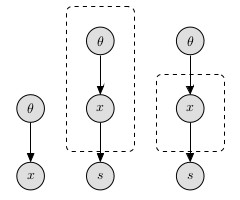
\includegraphics{plots/figure_A.jpg}
%DIFDELCMD < \end{center}
%DIFDELCMD < %%%
%DIFDELCMD < \caption{%
{%DIFAUXCMD
%DIFDELCMD < \label{fig:Plate notation, simple example} %%%
\DIFdelFL{Three simple selection models. }%DIFDELCMD < {\bf %%%
\DIFdelFL{(left)}%DIFDELCMD < } %%%
\DIFdelFL{the original $p(x,\theta)$; }%DIFDELCMD < {\bf %%%
\DIFdelFL{(middle)}%DIFDELCMD < } %%%
\DIFdelFL{the model $q_{\left\{ x,\theta\right\} }$, where $\theta$ and $x$ are
sampled together until $s=1$; }%DIFDELCMD < {\bf %%%
\DIFdelFL{(right)}%DIFDELCMD < } %%%
\DIFdelFL{the model $q_{x}$, where only $x$ is sampled until $s=1$.}}
%DIFAUXCMD
%DIFDELCMD < \end{figure}
%DIFDELCMD < 

%DIFDELCMD < %%%
\DIFdel{Let $f(x,\theta\mid\eta)=f(x\mid\theta,\eta)p(\theta)$
be the joint density of a random effects meta-analysis, where $x$ is the effect size, $\theta$ is the study-specific parameter of interest, and $\eta$ is a study-specific nuisance parameter such as the sample size of the study. The left plot of Figure \ref{fig:Plate notation, simple example} is a visualization of $f(x,\theta)$. If we have more than one study to analyse, we will have to work with product density $\prod_{i=1}^{n}f(x_{i},\theta_{i}\mid\eta_{i})$ instead of the stand-alone density $f(x,\theta\mid\eta)$. This is visualised in the middle plot of Figure \ref{fig:Plate notation, simple example}  by drawing a solid plate around the pair $(x,\theta)$. When we are dealing with a fixed effects meta-analysis, in which $\theta$ is fixed, the plate should be drawn around $x$ only (Figure \ref{fig:Plate notation, simple example}, right graph). 
}%DIFDELCMD < 

%DIFDELCMD < %%%
\subsection{\DIFdel{Publication bias and }\textit{\DIFdel{p}}%DIFAUXCMD
\DIFdel{-hacking models}%DIFDELCMD < \label{subsec:Selection sets, meta analysis}%%%
}
%DIFAUXCMD
\addtocounter{subsection}{-1}%DIFAUXCMD
%DIFDELCMD < 

%DIFDELCMD < %%%
\DIFdel{To visualize selection models based on }\textit{\DIFdel{p}}%DIFAUXCMD
\DIFdel{-values, we must make some modifications to the original graph: }%DIFDELCMD < 

%DIFDELCMD < \begin{enumerate}
\begin{enumerate}%DIFAUXCMD
%DIFDELCMD < \item[(i)] %%%
\item[\DIFdel{(i)}]%DIFAUXCMD
\DIFdel{Add the }\textit{\DIFdel{p}}%DIFAUXCMD
\DIFdel{-value node $u$.
}%DIFDELCMD < \item[(ii)] %%%
\item[\DIFdel{(ii)}]%DIFAUXCMD
\DIFdel{Add an arrow from $x$ to $u$. 
}%DIFDELCMD < \item[(iii)] %%%
\item[\DIFdel{(iii)}]%DIFAUXCMD
\DIFdel{Since the }\textit{\DIFdel{p}}%DIFAUXCMD
\DIFdel{-value $u$ usually depends on more information than just $x$, such as the standard deviation of $x$, add an arrow from $\eta$ (which represents the extra information) to $u$ as well.
}%DIFDELCMD < \item[(iv)] %%%
\item[\DIFdel{(iv)}]%DIFAUXCMD
\DIFdel{Add the selection node $s$ and an arrow from $u$ to $s$. If $u$ is the only parent of $s$, we are dealing with selection models only based on
}\textit{\DIFdel{p}}%DIFAUXCMD
\DIFdel{-values. }
\end{enumerate}%DIFAUXCMD
%DIFDELCMD < \end{enumerate}
%DIFDELCMD < 

%DIFDELCMD < %%%
\DIFdel{The placement of dashed and solid plates depends on which model we want to use. The }\DIFdelend \DIFaddbegin \DIFadd{a direct consequence of Proposition \ref{prop:Equal selection models}: the selection sets are different. The }\DIFaddend idea behind the publication bias model is that a completely new study is done whenever the last one failed to be published. This implies that \DIFdelbegin \DIFdel{$\theta$ }\DIFdelend \DIFaddbegin \DIFadd{each event of publication bias depends on the $\theta_i$ }\DIFaddend and \DIFdelbegin \DIFdel{$x$ are sampled together. The left plot of Figure \ref{fig:Plate notation, publication bias and p-hacking} shows the direct acyclic graph of the normal publication bias model defined in Proposition \ref{prop:One-sided normal discrete probability vector publication bias model-1}. In this particular case, $\eta$ corresponds to $\sigma$, the standard deviation. Moreover, $u$ is a }\textit{\DIFdel{p}}%DIFAUXCMD
\DIFdel{-value}\DIFdelend \DIFaddbegin \DIFadd{$x_i$ of the specific study. Moreover}\DIFaddend , \DIFdelbegin \DIFdel{$\theta_{0}$ is the mean of the effect size distribution, $\tau$ is the standard deviation of the effect size distribution, and $\rho$ is the selection probability function. The }\DIFdelend \DIFaddbegin \DIFadd{since the editor's decision to publish is also study-specific, the selection set also contains a }\DIFaddend variable $Z$\DIFdelbegin \DIFdel{lives }\DIFdelend \DIFaddbegin \DIFadd{, living }\DIFaddend on the unit interval, \DIFdelbegin \DIFdel{and encodes the editor's decision to publish}\DIFdelend \DIFaddbegin \DIFadd{that encodes her choice}\DIFaddend : If the observed \textit{p}-value is less than $Z$, the study is published. \DIFdelbegin \DIFdel{Importantly, $Z$ is placed inside the selection set because a new }\textit{\DIFdel{p}}%DIFAUXCMD
\DIFdel{-value cut-off decision is made for each study received. Since $x$ and $\theta$ }\DIFdelend \DIFaddbegin \DIFadd{Since $x_i$ and $\theta_i$ }\DIFaddend are sampled together, the selection mechanism modifies \DIFdelbegin \DIFdel{$p(\theta)$.
%DIF < , as can be seen in the example \ref{exa:Publication bias, theta distribution} here below.
}\DIFdelend \DIFaddbegin \DIFadd{$p(\theta_i)$.
}\DIFaddend 

In the \textit{p}-hacking scenario, the \textit{p}-hacker will hack his study all the way to significance, regardless of \DIFdelbegin \DIFdel{$\theta$}\DIFdelend \DIFaddbegin \DIFadd{$\theta_i$}\DIFaddend . This means that \DIFdelbegin \DIFdel{$\theta$ and $x$ are sampled separately and $\theta$ }\DIFdelend \DIFaddbegin \DIFadd{$\theta_i$ }\DIFaddend must be placed outside the selection set. Moreover, the decision of how much to \textit{p}-hack is not reevaluated at each attempt. Consequently, the random variable that controls the \textit{p}-hacking decisions, analogously to the publication bias model, $Z$, is also placed outside the selection \DIFdelbegin \DIFdel{graph}\DIFdelend \DIFaddbegin \DIFadd{set}\DIFaddend . This is the case, for example, of an author who decides to \textit{p}-hack to level $\alpha$ ($Z = \alpha$): he acts on \DIFdelbegin \DIFdel{$x$ }\DIFdelend \DIFaddbegin \DIFadd{$x_i$ }\DIFaddend to obtain the desired \textit{p}-value, whatever the sampled \DIFdelbegin \DIFdel{$\theta$ is. The graphical representation of this model is shown in the right plot of Figure \ref{fig:Plate notation, publication bias and p-hacking}. Since $x$ and $\theta$ are not sampled together}\DIFdelend \DIFaddbegin \DIFadd{$\theta_i$ is. Since $\theta_i$ does not belong to the selection set}\DIFaddend , the selection mechanism does not modify \DIFdelbegin \DIFdel{$p(\theta)$}\DIFdelend \DIFaddbegin \DIFadd{$p(\theta_i)$}\DIFaddend .

\DIFdelbegin %DIFDELCMD < \begin{figure}
%DIFDELCMD < \begin{center}
%DIFDELCMD < 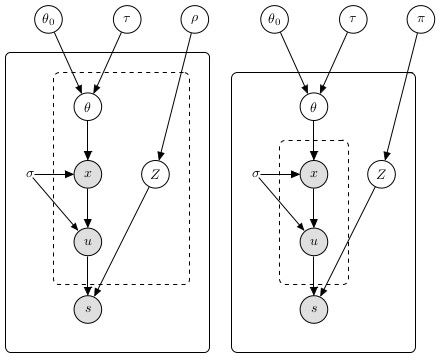
\includegraphics{plots/figure_B.jpg}
%DIFDELCMD < \end{center}
%DIFDELCMD < %%%
%DIFDELCMD < \caption{%
{%DIFAUXCMD
%DIFDELCMD < \label{fig:Plate notation, publication bias and p-hacking} %%%
\DIFdelFL{Directed acyclic graphs for: }%DIFDELCMD < {\bf %%%
\DIFdelFL{(left)}%DIFDELCMD < }
%DIFDELCMD < %%%
\DIFdelFL{the publication bias model; }%DIFDELCMD < {\bf %%%
\DIFdelFL{(right)}%DIFDELCMD < } %%%
\DIFdelFL{the }\textit{\DIFdelFL{p}}%DIFAUXCMD
\DIFdelFL{-hacking model. The dashed plates enclose the selection sets and the the solid plates enclose variables that are repeated together.}}
%DIFAUXCMD
%DIFDELCMD < \end{figure}
%DIFDELCMD < 

%DIFDELCMD < %%%
\subsection{\DIFdel{Equivalence in special cases}}
%DIFAUXCMD
\addtocounter{subsection}{-1}%DIFAUXCMD
\DIFdel{The }\DIFdelend \DIFaddbegin \DIFadd{The Web Appendix C contains an example that clarifies the different effect of the selection mechanism on $p(\theta_i)$ and a graphical representation of the two models, while the Web Appendix B a further proof of the model differences. The }\DIFaddend publication bias model defined in Proposition \ref{prop:One-sided normal discrete probability vector publication bias model-1} and the \textit{p}-hacking model are\DIFaddbegin \DIFadd{, indeed, }\DIFaddend equivalent when $\sigma_{i}$ is fixed across studies. This holds both for the fixed and random effects models. To see this, let $\pi$ be any probability vector for the \textit{p}-hacking model and solve the invertible linear system $\pi^{\star}(\rho)=\pi$ for $\rho$. There is no guarantee for the models to be equivalent when $\sigma_{i}$ is not fixed\DIFdelbegin \DIFdel{, see the appendix}\DIFdelend \DIFaddbegin \DIFadd{. Finally, Web Appendix D addresses the issue of identifiability, and shows that the two models are identifiable under weak conditions on $f$}\DIFaddend .


%DIF < \begin{example}[Publication Bias model with normal effect size distribution]
%DIF < 
%DIF < The density of the selected effect size distribution for the one-sided normal discrete probability vector publication bias model with normal effect size distribution is given in the following proposition.
%DIF < 
%DIF < The density of the selected effect size distribution for the one-sided
%DIF < normal discrete probability vector publication bias model with normal
%DIF < effect size distribution is
%DIF < 
%DIF < \[
%DIF < f_{sel}(\theta\mid\theta_{0},\tau,\sigma)=\phi(\theta\mid\theta_{0},\tau)\frac{\sum_{j=1}^{N}\rho_{j}\left[\Phi(c_{j-1}\mid\theta,\sigma)-\Phi(c_{j}\mid\theta,\sigma)\right]}{\sum_{j=1}^{N}\rho_{j}\left[(c_{j-1}\mid\theta_{0},\sqrt{\tau^{2}+\sigma^{2}})-\Phi(c_{j}\mid\theta_{0},\sqrt{\tau^{2}+\sigma^{2}})\right]}
%DIF < \]
%DIF < 
%DIF < By example \ref{exa:Publication bias, theta distribution}, $f(\theta\mid\theta_{0},\tau,\sigma)=\int\frac{p(s=1\mid x)}{p(s=1\mid\theta_{0},\tau,\sigma)}p(x,\theta\mid\theta_{0},\tau,\sigma)dx$.
%DIF < Then
%DIF < \[
%DIF < p(s=1\mid\theta_{0},\tau,\sigma)=\sum_{j=1}^{N}\rho_{j}\left[\Phi(c_{j-1}\mid\theta_{0},\sqrt{\tau^{2}+\sigma^{2}})-\Phi(c_{j}\mid\theta_{0},\sqrt{\tau^{2}+\sigma^{2}})\right],
%DIF < \]
%DIF < with $c_{j}=\Phi^{-1}(1-\alpha_{j})$. Since $p(s=1\mid x)=\sum_{j=1}^{N}\rho_{j}1_{\left[c_{j},c_{j-1})}(x)$
%DIF < and $p(x,\theta\mid\theta_{0},\tau,\sigma)=\phi(x\mid\theta,\sigma)\phi(\theta\mid\theta_{0},\tau)$,
%DIF < \begin{eqnarray*}
%DIF < \int p(s=1\mid x)p(x,\theta\mid\theta_{0},\tau,\sigma)dx & = & \phi(\theta\mid\theta_{0},\tau)\sum_{j=1}^{N}\rho_{j}\left[\Phi(c_{j-1}\mid\theta,\sigma)-\Phi(c_{j}\mid\theta,\sigma)\right]
%DIF < \end{eqnarray*}
%DIF < 
%DIF < Since the selected effect size distribution depends on the \textit{p}-value
%DIF < $u$, it also depends on $\sigma$. Since we never run a meta-analysis
%DIF < on just on data point, we will always have a collection of $\sigma$s
%DIF < to deal with. Define the \emph{observed effect size density }by 
%DIF < \begin{equation}
%DIF < f_{obs}(\theta\mid\theta_{0},\tau,\left\{ \sigma_{i}\right\} _{i=1}^{n})=\sum_{i=1}^{n}\frac{1}{n}f_{sel}(\theta\mid\theta_{0},\tau,\sigma_{i})\label{eq:Observed effect size density}
%DIF < \end{equation}
%DIF < This is the mean of the the selected effect size distribution, and
%DIF < is interpreted as the selected effect size distribution when $\sigma_{i}$
%DIF < is chosen randomly among the collection of $\sigma$s. The observed
%DIF < effect size distribution can be widely different from the underlying
%DIF < effect size distribution, as we will see in section \ref{subsec:cuddy2018}.
%DIF < \end{example}
\DIFdelbegin %DIFDELCMD < 

%DIFDELCMD < %%%
\DIFdelend \section{Simulations}\label{sect:simulations}

%DIF < \begin{example}[Publication bias selected effect size distribution]\label{exa:Publication bias, theta distribution}
%DIF < The density of $\theta$ in a random effects meta-analysis with publication bias is $\int\frac{p(s=1\mid u)}{p(s=1\mid\theta;\eta)}p(x,\theta;\eta)dx$, where $\eta$ are study-specific parameters and $u$ is a deterministic function of $x$ and $\eta$. Since $u$ typically depends on both
%DIF < $x$ and $\eta$, so does the density of $\theta$. Let $x$ be normal with mean $\theta$ and standard deviation $\sigma$, $u$ be the usual one-sided \textit{p}-value and the effect size distribution of $\theta$ be normal with mean $\theta_{0}$ and standard deviation $\tau$, the setting of example \ref{prop:One-sided normal discrete probability vector publication bias model-1}. The selection mechanism $s$ equals $1$ when $u\leq0.05$ and $p(s=1)=0.1$ otherwise. This means that every significant study is published and a non-significant study is published with probability $0.1$.
%DIF < 
%DIF < The effect of publication bias on the distribution of $\theta$ is shown in Figure \ref{fig:Marginal distribution of effect sizes}. Two selected effect size distributions with underlying mean $0$ are displayed: one with a large standard deviation (left plot, $\tau=0.5$) and one with a small one ($\tau=0.1$, right plot). In both cases, the effect of the selection is shown with two different values $\sigma$, namely $1/100$ (dashed line) and $1/20$ (dotted line). The effect size distribution is strongly affected by $\tau$ both in shape and location; the mean of the selected distribution when $\tau = 0.5$ is $0.5$ when $\sigma=1/100$ and $0.58$ when $\sigma=1/20$. When $\tau = 0.1$, the mean of the selected distribution is $0.08$ when $\sigma=1/100$ and $0.12$ when $\sigma=1/20$. Thus, while $\sigma$ has an effect on the shape and mean of the selected distribution, it is much smaller than the effect of $\tau$.
%DIF < 
%DIF < \begin{figure}
%DIF < \noindent \begin{centering}
%DIF < \includegraphics[scale=0.3]{plots/pb_esdistribution_large_tau}\includegraphics[scale=0.3]{plots/pb_esdistribution_small_tau}
%DIF < \par\end{centering}
%DIF < \caption{\label{fig:Marginal distribution of effect sizes} The distribution of $\theta$ before and after selection. In both plots, $\theta_{0}=0$, the solid line is the effect sizes distribution before selection,
%DIF < the dashed line selected with $\sigma^{2}=1/100$ and the dotted line
%DIF < selected with $\sigma^{2}=1/20$ and. (left) $\tau=0.5$ (right) $\tau=0.1$.
%DIF < Notice the change of $y$-axis.}
%DIF < \end{figure}
%DIF < \end{example}
%DIF < 
%DIF < 
%DIF < \subsection{Publication bias model versus \textit{p}-hacking model}
We want to answer these three questions about the \textit{p}-hacking and publication bias models: \DIFdelbegin %DIFDELCMD < \begin{enumerate}
%DIFDELCMD < \item %%%
\DIFdelend \DIFaddbegin \DIFadd{(1) }\DIFaddend Do they work even in the absence of \textit{p}-hacking and publication bias? Although we know these phenomena are ubiquitous and should always be corrected for, it is still important that the models do not distort the results when there is no publication bias or \textit{p}-hacking. \DIFdelbegin %DIFDELCMD < \item %%%
\DIFdelend \DIFaddbegin \DIFadd{(2) }\DIFaddend How do they behave in extreme situations\DIFdelbegin \DIFdel{? In particular, we are interested in how the models behave }\DIFdelend \DIFaddbegin \DIFadd{, in particular }\DIFaddend when $n$ is small and the heterogeneity is large\DIFdelbegin \DIFdel{.
}%DIFDELCMD < \item %%%
\DIFdelend \DIFaddbegin \DIFadd{? (3) }\DIFaddend Are the models distinguishable in practice? Does the \textit{p}-hacking model work under the publication bias scenario and vice versa?
\DIFdelbegin %DIFDELCMD < \end{enumerate}
%DIFDELCMD < %%%
\DIFdelend 

\subsection{Settings}
We generate data under three scenarios: (i) With no publication bias nor \textit{p}-hacking, using the normal random effect meta-analysis model. (ii) Under the presence of publication bias, using model \eqref{eq:Random effects, publication bias}. (iii) Under presence of \textit{p}-hacking, using the random effects normal \textit{p}-hacking model. The study-specific variances $\sigma_{i}^{2}$ are sampled uniformly from $\left\{ 20,\ldots80\right\} $. The size of the meta-analyses are $n = 5, 30, 100$, corresponding to small, medium and large meta-analyses, while the means for the effect size distribution are $0, 0.2, 0.8$. The value $\theta_0 = 0$ corresponds to no expected effect, while the positive $\theta_0$s are the cut-off for small and large effect sizes of \citet[][pages 24 -- 27]{cohen1988statistical}. The standard deviations of the random effects distributions are $\tau=0.1$ and $\tau=0.5$. While $\tau = 0.1$ is a reasonable amount of heterogeneity, $\tau=0.5$ is a large amount of heterogeneity that provides a challenge for the models. The probability of acceptance of a paper are simulated to be $1$ if the \textit{p}-value is between $0$ and $0.025$, $0.7$ if the \textit{p}-value is between $0.025$ and $0.05$, and $0.1$ otherwise. For the same intervals, the \textit{p}-hacking probabilities are $0.6$, $0.3$ and $0.1$. 

\DIFdelbegin \DIFdel{For }\DIFdelend \DIFaddbegin \DIFadd{In addition to the classical uncorrected model for meta-analysis, for }\DIFaddend each parameter combination we estimate the \textit{p}-hacking model and the publication bias model \DIFdelbegin \DIFdel{. Both }\DIFdelend \DIFaddbegin \DIFadd{using Bayesian methods. While a frequentist approach is in theory possible, it may lead to poor results if ad-hoc penalizations or bias corrections are not implemented. See  \mbox{%DIFAUXCMD
\citet[Appendix, 1]{mcshane2016adjusting} }\hspace{0pt}%DIFAUXCMD
and \mbox{%DIFAUXCMD
\citet{Moss2019} }\hspace{0pt}%DIFAUXCMD
for further details. All }\DIFaddend models have normal likelihoods and normal effect size distributions. We use one-sided significance cut-offs at $0.025$ and $0.05$ for both the publication bias and the \textit{p}-hacking models. We use standard \DIFdelbegin \DIFdel{Gaussian }\DIFdelend \DIFaddbegin \DIFadd{normal }\DIFaddend priors for $\theta_0$, a standard half normal prior for $\tau$, and, in the \textit{p}-hacking model, a uniform Dirichlet prior for $\pi$. For the $\rho$ in the publication bias model we use a a uniform Dirichlet that constrains \DIFdelbegin \DIFdel{$\rho_{1}\geq\rho_{2}\geq\ldots\geq\rho_{j}$}\DIFdelend \DIFaddbegin \DIFadd{$\rho_{1}\geq\ldots\geq\rho_{j}$}\DIFaddend . That is, the publication probability is a decreasing function of the \textit{p}-value.

All of these priors are reasonable. A standard normal for $\theta_0$ is reasonable because we know that $\theta_0$ has a small magnitude in pretty much any meta-analysis, and most are clustered around $0$. A half normal prior for $\tau$ is also reasonable, as $\tau$ is much more likely to be very small than very big. The priors for $\rho$ and $\pi$ are harder to reason about, but a uniform Dirichlet seems like a natural and neutral choice. These are the standard prior of the $\mathtt{R}$ package $\mathtt{publipha}$ \citep{publipha}, which we used for all computations. $\mathtt{publipha}$ uses $\mathtt{STAN}$ \citep{Carpenter2017-cf} to estimate the models, and each estimation uses $8$ chains.

The number of simulations is $N = 100$ for each parameter combination. \DIFdelbegin \DIFdel{See the OSF repository for this paper (}%DIFDELCMD < \url{https://osf.io/tx8qn/}%%%
\DIFdel{) for the }\DIFdelend \DIFaddbegin \DIFadd{The }\DIFaddend code used to run the simulations \DIFdelbegin \DIFdel{and its raw data}\DIFdelend \DIFaddbegin \DIFadd{is available in the Online Supporting Information and in an OSF repository (}\url{https://osf.io/tx8qn/}\DIFadd{)}\DIFaddend .

\subsection{Results}
\paragraph{No publication bias, no \textit{p}-hacking.} The results under this scenario are reported in Table \ref{tab:Simulation_classical}. When the amount of heterogeneity is reasonable ($\tau = 0.1$) both the \textit{p}-hacking and the publication bias perform well. The publication bias model performs slightly worse than the \textit{p}-hacking model when the mean effect size is large ($\theta_0 = 0.8$) and the number of studies small ($n=5$), but it catches up as $n$ increases. \DIFdelbegin \DIFdel{The situation with }\DIFdelend \DIFaddbegin \DIFadd{With }\DIFaddend $\tau = 0.5$\DIFdelbegin \DIFdel{is more interesting. Here }\DIFdelend \DIFaddbegin \DIFadd{, }\DIFaddend the \textit{p}-hacking model outperforms the publication bias model, with the latter tending to underestimate the mean effect. While increasing $n$ alleviates the problem, there is still a substantial underestimation of $\theta_0$ even in the case of $n = 100$. In contrast, both models \DIFdelbegin \DIFdel{seems }\DIFdelend \DIFaddbegin \DIFadd{seem }\DIFaddend to estimate $\tau$ pretty well. \DIFdelbegin \DIFdel{As a take home message, it is safe to use the }\textit{\DIFdel{p}}%DIFAUXCMD
\DIFdel{-hacking model when there is no }\textit{\DIFdel{p}}%DIFAUXCMD
\DIFdel{-hacking or publication bias , but less safe to use the publication bias model }\DIFdelend \DIFaddbegin \DIFadd{Obviously, without any publication bias or $p$-hacking, the classical uncorrected model gives good results}\DIFaddend .

\begin{table}[ht]
\centering
\DIFaddendFL \caption{\DIFdelbeginFL %DIFDELCMD < \label{tab:Simulation_classical} %%%
\DIFdelendFL {\bf No publication bias, no 
                    \textit{p}-hacking.} Posterior means 
                    and standard deviations from the \textit{p}-hacking\DIFdelbeginFL \DIFdelFL{and }\DIFdelendFL \DIFaddbeginFL \DIFaddFL{, 
                    }\DIFaddendFL publication bias\DIFaddbeginFL \DIFaddFL{, and uncorrected }\DIFaddendFL models when the data are simulated 
                    from the normal random effects meta-analysis model.} 
\label{tab:Simulation_classical}
\begin{tabular}{lllrrrrrr}
   \DIFaddendFL \multicolumn{3}{r}{\textbf{True values}} & 
       \DIFaddbeginFL \multicolumn{2}{c}{\textbf{\textit{p}-hacking model}} \DIFaddendFL &
       \DIFdelbeginFL %DIFDELCMD < \multicolumn{3}{c}{\textbf{\textit{p}-hacking model}} %%%
\DIFdelendFL \DIFaddbeginFL \multicolumn{2}{c}{\textbf{Publication bias model}} \DIFaddendFL &
       \DIFdelbeginFL %DIFDELCMD < & \multicolumn{3}{c}{\textbf{Publication bias model}} & \tabularnewline
%DIFDELCMD < %%%
\DIFdelendFL \DIFaddbeginFL \multicolumn{2}{c}{\textbf{Uncorrected model}}\\\DIFaddendFL $\tau$ & $\theta_0$ & $n$ & \DIFdelbeginFL %DIFDELCMD < & %%%
\DIFdelendFL \multicolumn{1}{c}{$\widehat{\theta_0}$} & \DIFdelbeginFL %DIFDELCMD < & %%%
\DIFdelendFL \multicolumn{1}{c}{$\widehat{\tau}$} & \DIFdelbeginFL %DIFDELCMD < & %%%
\DIFdelendFL \multicolumn{1}{c}{$\widehat{\theta_0}$} & \DIFdelbeginFL %DIFDELCMD < & %%%
\DIFdelendFL \multicolumn{1}{c}{$\widehat{\tau}$} & \DIFdelbeginFL %DIFDELCMD < \tabularnewline
%DIFDELCMD < %%%
\DIFdelendFL \DIFaddbeginFL \multicolumn{1}{c}{$\widehat{\theta_0}$} & \multicolumn{1}{c}{$\widehat{\tau}$} \\ 
   \DIFaddendFL \hline
\multirow{9}{*}{$0.1$} & \multirow{3}{*}{$0$} & \DIFdelbeginFL \DIFdelFL{$5$ }\DIFdelendFL \DIFaddbeginFL \DIFaddFL{5 }\DIFaddendFL & \DIFdelbeginFL %DIFDELCMD < & %%%
\DIFdelendFL -0.03 (0.09) & \DIFdelbeginFL %DIFDELCMD < & %%%
\DIFdelendFL 0.18 (0.07) & \DIFdelbeginFL %DIFDELCMD < & %%%
\DIFdelendFL -0.06 (0.08) & \DIFdelbeginFL %DIFDELCMD < & %%%
\DIFdelendFL 0.13 (0.06) & \DIFdelbeginFL %DIFDELCMD < \tabularnewline
%DIFDELCMD <  %%%
\DIFdelendFL \DIFaddbeginFL \DIFaddFL{0.00 (0.09) }\DIFaddendFL & \DIFaddbeginFL \DIFaddFL{0.19 (0.08) }\\ 
   \DIFaddendFL &  \DIFdelbeginFL \DIFdelFL{$30$ }\DIFdelendFL & \DIFaddbeginFL \DIFaddFL{30 }\DIFaddendFL & -0.01 (0.03) & \DIFdelbeginFL %DIFDELCMD < & %%%
\DIFdelendFL 0.08 (0.03) & \DIFdelbeginFL %DIFDELCMD < & %%%
\DIFdelendFL -0.02 (0.03) & \DIFdelbeginFL %DIFDELCMD < & %%%
\DIFdelendFL 0.07 (0.03) & \DIFdelbeginFL %DIFDELCMD < \tabularnewline
%DIFDELCMD <  %%%
\DIFdelendFL \DIFaddbeginFL \DIFaddFL{0.00 (0.04) }\DIFaddendFL & \DIFaddbeginFL \DIFaddFL{0.10 (0.04) }\\ 
   \DIFaddendFL &  \DIFdelbeginFL \DIFdelFL{$100$ }\DIFdelendFL & \DIFaddbeginFL \DIFaddFL{100 }\DIFaddendFL & -0.01 (0.02) & \DIFdelbeginFL %DIFDELCMD < & %%%
\DIFdelendFL 0.08 (0.03) & \DIFdelbeginFL %DIFDELCMD < & %%%
\DIFdelendFL -0.01 (0.02) & \DIFdelbeginFL %DIFDELCMD < & %%%
\DIFdelendFL 0.07 (0.02) & \DIFdelbeginFL %DIFDELCMD < \tabularnewline
%DIFDELCMD <  \cdashline{3-11}
%DIFDELCMD <  %%%
\DIFdelendFL \DIFaddbeginFL \DIFaddFL{0.00 (0.02) }\DIFaddendFL & \DIFaddbeginFL \DIFaddFL{0.10 (0.03) }\\ 
   \cdashline{3-9}
 & \DIFaddendFL \multirow{3}{*}{$0.2$} & \DIFdelbeginFL \DIFdelFL{$5$ }\DIFdelendFL \DIFaddbeginFL \DIFaddFL{5 }\DIFaddendFL & \DIFdelbeginFL %DIFDELCMD < &  %%%
\DIFdelendFL 0.12 (0.08) & \DIFdelbeginFL %DIFDELCMD < & %%%
\DIFdelendFL 0.21 (0.08) & \DIFdelbeginFL %DIFDELCMD < &  %%%
\DIFdelendFL 0.09 (0.07) & \DIFdelbeginFL %DIFDELCMD < & %%%
\DIFdelendFL 0.17 (0.08) & \DIFdelbeginFL %DIFDELCMD < \tabularnewline
%DIFDELCMD <  %%%
\DIFdelendFL \DIFaddbeginFL \DIFaddFL{0.20 (0.08) }\DIFaddendFL & \DIFaddbeginFL \DIFaddFL{0.19 (0.08) }\\ 
   \DIFaddendFL &  \DIFdelbeginFL \DIFdelFL{$30$ }\DIFdelendFL & \DIFaddbeginFL \DIFaddFL{30 }\DIFaddendFL & 0.17 (0.04) & \DIFdelbeginFL %DIFDELCMD < & %%%
\DIFdelendFL 0.09 (0.04) & \DIFdelbeginFL %DIFDELCMD < &  %%%
\DIFdelendFL 0.15 (0.03) & \DIFdelbeginFL %DIFDELCMD < & %%%
\DIFdelendFL 0.09 (0.04) & \DIFdelbeginFL %DIFDELCMD < \tabularnewline
%DIFDELCMD <  %%%
\DIFdelendFL \DIFaddbeginFL \DIFaddFL{0.20 (0.03) }\DIFaddendFL & \DIFaddbeginFL \DIFaddFL{0.10 (0.04) }\\ 
   \DIFaddendFL &  \DIFdelbeginFL \DIFdelFL{$100$ }\DIFdelendFL & \DIFaddbeginFL \DIFaddFL{100 }\DIFaddendFL & 0.18 (0.02) & \DIFdelbeginFL %DIFDELCMD < & %%%
\DIFdelendFL 0.09 (0.03) & \DIFdelbeginFL %DIFDELCMD < &  %%%
\DIFdelendFL 0.17 (0.02) & \DIFdelbeginFL %DIFDELCMD < & %%%
\DIFdelendFL 0.09 (0.03) & \DIFdelbeginFL %DIFDELCMD < \tabularnewline
%DIFDELCMD <  \cdashline{3-11}
%DIFDELCMD <  %%%
\DIFdelendFL \DIFaddbeginFL \DIFaddFL{0.20 (0.02) }\DIFaddendFL & \DIFaddbeginFL \DIFaddFL{0.10 (0.02) }\\ 
   \cdashline{3-9}
 & \DIFaddendFL \multirow{3}{*}{$0.8$} & \DIFdelbeginFL \DIFdelFL{$5$ }\DIFdelendFL \DIFaddbeginFL \DIFaddFL{5 }\DIFaddendFL & \DIFdelbeginFL %DIFDELCMD < &  %%%
\DIFdelendFL 0.78 (0.08) & \DIFdelbeginFL %DIFDELCMD < & %%%
\DIFdelendFL 0.21 (0.10) & \DIFdelbeginFL %DIFDELCMD < &  %%%
\DIFdelendFL 0.63 (0.15) & \DIFdelbeginFL %DIFDELCMD < & %%%
\DIFdelendFL 0.34 (0.14) & \DIFdelbeginFL %DIFDELCMD < \tabularnewline
%DIFDELCMD <  %%%
\DIFdelendFL \DIFaddbeginFL \DIFaddFL{0.79 (0.07) }\DIFaddendFL & \DIFaddbeginFL \DIFaddFL{0.20 (0.08) }\\ 
   \DIFaddendFL &  \DIFdelbeginFL \DIFdelFL{$30$ }\DIFdelendFL & \DIFaddbeginFL \DIFaddFL{30 }\DIFaddendFL & 0.80 (0.04) & \DIFdelbeginFL %DIFDELCMD < & %%%
\DIFdelendFL 0.11 (0.04) & \DIFdelbeginFL %DIFDELCMD < &  %%%
\DIFdelendFL 0.80 (0.04) & \DIFdelbeginFL %DIFDELCMD < & %%%
\DIFdelendFL 0.11 (0.04) & \DIFdelbeginFL %DIFDELCMD < \tabularnewline
%DIFDELCMD <  %%%
\DIFdelendFL \DIFaddbeginFL \DIFaddFL{0.80 (0.04) }\DIFaddendFL & \DIFaddbeginFL \DIFaddFL{0.10 (0.04) }\\ 
   \DIFaddendFL &  \DIFdelbeginFL \DIFdelFL{$100$ }\DIFdelendFL & \DIFaddbeginFL \DIFaddFL{100 }\DIFaddendFL & 0.80 (0.02) & \DIFdelbeginFL %DIFDELCMD < & %%%
\DIFdelendFL 0.10 (0.03) & \DIFdelbeginFL %DIFDELCMD < &  %%%
\DIFdelendFL 0.80 (0.02) & \DIFdelbeginFL %DIFDELCMD < & %%%
\DIFdelendFL 0.10 (0.03) & \DIFdelbeginFL %DIFDELCMD < \tabularnewline
%DIFDELCMD <  \cline{2-12}
%DIFDELCMD < %%%
\DIFdelendFL \DIFaddbeginFL \DIFaddFL{0.80 (0.02) }& \DIFaddFL{0.09 (0.03) }\\ 
   \cline{2-9}
\DIFaddendFL \multirow{9}{*}{$0.5$} & \multirow{3}{*}{$0$} & \DIFdelbeginFL \DIFdelFL{$5$ }\DIFdelendFL \DIFaddbeginFL \DIFaddFL{5 }\DIFaddendFL & \DIFdelbeginFL %DIFDELCMD < & %%%
\DIFdelendFL -0.03 (0.20) & \DIFdelbeginFL %DIFDELCMD < & %%%
\DIFdelendFL 0.59 (0.21) & \DIFdelbeginFL %DIFDELCMD < & %%%
\DIFdelendFL -0.21 (0.17) & \DIFdelbeginFL %DIFDELCMD < & %%%
\DIFdelendFL 0.53 (0.21) & \DIFdelbeginFL %DIFDELCMD < \tabularnewline
%DIFDELCMD <  %%%
\DIFdelendFL \DIFaddbeginFL \DIFaddFL{0.01 (0.20) }\DIFaddendFL & \DIFaddbeginFL \DIFaddFL{0.61 (0.20) }\\ 
   \DIFaddendFL &  \DIFdelbeginFL \DIFdelFL{$30$ }\DIFdelendFL & \DIFaddbeginFL \DIFaddFL{30 }\DIFaddendFL & -0.03 (0.09) & \DIFdelbeginFL %DIFDELCMD < & %%%
\DIFdelendFL 0.51 (0.08) & \DIFdelbeginFL %DIFDELCMD < & %%%
\DIFdelendFL -0.14 (0.09) & \DIFdelbeginFL %DIFDELCMD < & %%%
\DIFdelendFL 0.47 (0.08) & \DIFdelbeginFL %DIFDELCMD < \tabularnewline
%DIFDELCMD <  %%%
\DIFdelendFL \DIFaddbeginFL \DIFaddFL{-0.01 (0.09) }\DIFaddendFL & \DIFaddbeginFL \DIFaddFL{0.51 (0.07) }\\ 
   \DIFaddendFL &  \DIFdelbeginFL \DIFdelFL{$100$ }\DIFdelendFL & \DIFaddbeginFL \DIFaddFL{100 }\DIFaddendFL & -0.02 (0.05) & \DIFdelbeginFL %DIFDELCMD < & %%%
\DIFdelendFL 0.50 (0.04) & \DIFdelbeginFL %DIFDELCMD < & %%%
\DIFdelendFL -0.08 (0.06) & \DIFdelbeginFL %DIFDELCMD < & %%%
\DIFdelendFL 0.48 (0.04) & \DIFdelbeginFL %DIFDELCMD < \tabularnewline
%DIFDELCMD <  \cdashline{3-11}
%DIFDELCMD <  %%%
\DIFdelendFL \DIFaddbeginFL \DIFaddFL{0.00 (0.05) }\DIFaddendFL & \DIFaddbeginFL \DIFaddFL{0.50 (0.04) }\\ 
   \cdashline{3-9}
 & \DIFaddendFL \multirow{3}{*}{$0.2$} & \DIFdelbeginFL \DIFdelFL{$5$ }\DIFdelendFL \DIFaddbeginFL \DIFaddFL{5 }\DIFaddendFL & \DIFdelbeginFL %DIFDELCMD < &  %%%
\DIFdelendFL 0.10 (0.22) & \DIFdelbeginFL %DIFDELCMD < & %%%
\DIFdelendFL 0.57 (0.20) & \DIFdelbeginFL %DIFDELCMD < & %%%
\DIFdelendFL -0.09 (0.19) & \DIFdelbeginFL %DIFDELCMD < & %%%
\DIFdelendFL 0.54 (0.19) & \DIFdelbeginFL %DIFDELCMD < \tabularnewline
%DIFDELCMD <  %%%
\DIFdelendFL \DIFaddbeginFL \DIFaddFL{0.16 (0.21) }\DIFaddendFL & \DIFaddbeginFL \DIFaddFL{0.58 (0.19) }\\ 
   \DIFaddendFL &  \DIFdelbeginFL \DIFdelFL{$30$ }\DIFdelendFL & \DIFaddbeginFL \DIFaddFL{30 }\DIFaddendFL & 0.15 (0.10) & \DIFdelbeginFL %DIFDELCMD < & %%%
\DIFdelendFL 0.53 (0.08) & \DIFdelbeginFL %DIFDELCMD < &  %%%
\DIFdelendFL 0.02 (0.10) & \DIFdelbeginFL %DIFDELCMD < & %%%
\DIFdelendFL 0.51 (0.08) & \DIFdelbeginFL %DIFDELCMD < \tabularnewline
%DIFDELCMD <  %%%
\DIFdelendFL \DIFaddbeginFL \DIFaddFL{0.19 (0.10) }\DIFaddendFL & \DIFaddbeginFL \DIFaddFL{0.52 (0.08) }\\ 
   \DIFaddendFL &  \DIFdelbeginFL \DIFdelFL{$100$ }\DIFdelendFL & \DIFaddbeginFL \DIFaddFL{100 }\DIFaddendFL & 0.19 (0.05) & \DIFdelbeginFL %DIFDELCMD < & %%%
\DIFdelendFL 0.51 (0.04) & \DIFdelbeginFL %DIFDELCMD < &  %%%
\DIFdelendFL 0.11 (0.06) & \DIFdelbeginFL %DIFDELCMD < & %%%
\DIFdelendFL 0.49 (0.04) & \DIFdelbeginFL %DIFDELCMD < \tabularnewline
%DIFDELCMD <  \cdashline{3-11}
%DIFDELCMD <  %%%
\DIFdelendFL \DIFaddbeginFL \DIFaddFL{0.21 (0.05) }\DIFaddendFL & \DIFaddbeginFL \DIFaddFL{0.50 (0.04) }\\ 
   \cdashline{3-9}
 & \DIFaddendFL \multirow{3}{*}{$0.8$} & \DIFdelbeginFL \DIFdelFL{$5$ }\DIFdelendFL \DIFaddbeginFL \DIFaddFL{5 }\DIFaddendFL & \DIFdelbeginFL %DIFDELCMD < &  %%%
\DIFdelendFL 0.68 (0.23) & \DIFdelbeginFL %DIFDELCMD < & %%%
\DIFdelendFL 0.62 (0.21) & \DIFdelbeginFL %DIFDELCMD < &  %%%
\DIFdelendFL 0.35 (0.23) & \DIFdelbeginFL %DIFDELCMD < & %%%
\DIFdelendFL 0.74 (0.21) & \DIFdelbeginFL %DIFDELCMD < \tabularnewline
%DIFDELCMD <  %%%
\DIFdelendFL \DIFaddbeginFL \DIFaddFL{0.72 (0.21) }\DIFaddendFL & \DIFaddbeginFL \DIFaddFL{0.59 (0.21) }\\ 
   \DIFaddendFL &  \DIFdelbeginFL \DIFdelFL{$30$ }\DIFdelendFL & \DIFaddbeginFL \DIFaddFL{30 }\DIFaddendFL & 0.78 (0.10) & \DIFdelbeginFL %DIFDELCMD < & %%%
\DIFdelendFL 0.52 (0.08) & \DIFdelbeginFL %DIFDELCMD < &  %%%
\DIFdelendFL 0.60 (0.14) & \DIFdelbeginFL %DIFDELCMD < & %%%
\DIFdelendFL 0.60 (0.08) & \DIFdelbeginFL %DIFDELCMD < \tabularnewline
%DIFDELCMD <  %%%
\DIFdelendFL \DIFaddbeginFL \DIFaddFL{0.80 (0.09) }\DIFaddendFL & \DIFaddbeginFL \DIFaddFL{0.50 (0.07) }\\ 
   \DIFaddendFL &  \DIFdelbeginFL \DIFdelFL{$100$ }\DIFdelendFL & \DIFaddbeginFL \DIFaddFL{100 }\DIFaddendFL & 0.79 (0.05) & \DIFdelbeginFL %DIFDELCMD < & %%%
\DIFdelendFL 0.51 (0.04) & \DIFdelbeginFL %DIFDELCMD < &  %%%
\DIFdelendFL 0.70 (0.07) & \DIFdelbeginFL %DIFDELCMD < & %%%
\DIFdelendFL 0.55 (0.04) & \DIFdelbeginFL %DIFDELCMD < \tabularnewline
%DIFDELCMD <  %%%
\DIFdelendFL \DIFaddbeginFL \DIFaddFL{0.80 (0.05) }& \DIFaddFL{0.50 (0.04) }\\ 
   \DIFaddendFL \hline
\end{tabular}
\end{table}

\paragraph{Publication bias\DIFdelbegin \DIFdel{.}\DIFdelend } Overall, the publication bias model outperforms the \textit{p}-hacking model when the data are generated from the publication bias model, but not by much, see Table \ref{tab:Simulation_pb}\DIFdelbegin \DIFdel{)}\DIFdelend . When $\tau = 0.5$ the \textit{p}-hacking model tends to overestimates $\theta_0$ while the publication bias model tends to underestimate it\DIFdelbegin \DIFdel{, and the }\DIFdelend \DIFaddbegin \DIFadd{. The }\DIFaddend overestimation of the \textit{p}-hacking model is most extreme when $\theta_0 = 0.2$\DIFaddbegin \DIFadd{, but not as strong as the classical uncorrected model}\DIFaddend . When $\tau = 0.1$, the \DIFaddbegin \DIFadd{publication bias and $p$-hacking }\DIFaddend models produce almost indistinguishable results\DIFdelbegin \DIFdel{. In the most challenging case of $n=5$, the }\textit{\DIFdel{p}}%DIFAUXCMD
\DIFdel{-hacking model is never worse than the publication bias model and is closer to the truth when $\theta_0 = 0.8$}\DIFdelend \DIFaddbegin \DIFadd{, ouperforming the uncorrected model (especially if the effect $\theta_0$ is null or small)}\DIFaddend . Just as in the \textit{p}-hacking scenario, both models estimate $\tau$ reasonably well.

\begin{table}[ht]
\centering
\DIFaddendFL \caption{\DIFdelbeginFL %DIFDELCMD < \label{tab:Simulation_pb} %%%
\DIFdelendFL {\bf Publication bias.} 
                    Posterior means and standard deviations from the 
                    \textit{p}-hacking\DIFdelbeginFL \DIFdelFL{and }\DIFdelendFL \DIFaddbeginFL \DIFaddFL{, }\DIFaddendFL publication bias\DIFaddbeginFL \DIFaddFL{, and uncorrected }\DIFaddendFL models 
                    when the data are simulated from the publication 
                    bias model with cut-offs at $0.025$ and $0.05$, 
                    with selection probabilities equal to $1$, $0.7$, 
                    and $0.1$ in the intervals $[0, 0.025)$, $[0.025, 0.05)$, 
                    and $[0.5, 1]$.} 
\label{tab:Simulation_pb}
\begin{tabular}{lllrrrrrr}
   \DIFaddendFL \multicolumn{3}{r}{\textbf{True values}} & 
       \DIFaddbeginFL \multicolumn{2}{c}{\textbf{\textit{p}-hacking model}} \DIFaddendFL &
       \DIFdelbeginFL %DIFDELCMD < \multicolumn{3}{c}{\textbf{\textit{p}-hacking model}} %%%
\DIFdelendFL \DIFaddbeginFL \multicolumn{2}{c}{\textbf{Publication bias model}} \DIFaddendFL &
       \DIFdelbeginFL %DIFDELCMD < & \multicolumn{3}{c}{\textbf{Publication bias model}} & \tabularnewline
%DIFDELCMD < %%%
\DIFdelendFL \DIFaddbeginFL \multicolumn{2}{c}{\textbf{Uncorrected model}}\\\DIFaddendFL $\tau$ & $\theta_0$ & $n$ & \DIFaddbeginFL \multicolumn{1}{c}{$\widehat{\theta_0}$} \DIFaddendFL & \DIFdelbeginFL \DIFdelFL{$\widehat{\theta_0}$ }\DIFdelendFL \DIFaddbeginFL \multicolumn{1}{c}{$\widehat{\tau}$} \DIFaddendFL & \DIFaddbeginFL \multicolumn{1}{c}{$\widehat{\theta_0}$} \DIFaddendFL & \DIFdelbeginFL \DIFdelFL{$\widehat{\tau}$ }\DIFdelendFL \DIFaddbeginFL \multicolumn{1}{c}{$\widehat{\tau}$} \DIFaddendFL & \DIFaddbeginFL \multicolumn{1}{c}{$\widehat{\theta_0}$} \DIFaddendFL & \DIFdelbeginFL \DIFdelFL{$\widehat{\theta_0}$ }%DIFDELCMD < &  & %%%
\DIFdelFL{$\widehat{\tau}$ }%DIFDELCMD < & \tabularnewline
%DIFDELCMD < %%%
\DIFdelendFL \DIFaddbeginFL \multicolumn{1}{c}{$\widehat{\tau}$} \\ 
   \DIFaddendFL \hline
\multirow{9}{*}{$0.1$} & \multirow{3}{*}{$0$} & \DIFdelbeginFL \DIFdelFL{$5$ }\DIFdelendFL \DIFaddbeginFL \DIFaddFL{5 }\DIFaddendFL & \DIFdelbeginFL %DIFDELCMD < & %%%
\DIFdelendFL -0.01 (0.10) & \DIFdelbeginFL %DIFDELCMD < & %%%
\DIFdelendFL 0.23 (0.08) & \DIFdelbeginFL %DIFDELCMD < & %%%
\DIFdelendFL -0.01 (0.07) & \DIFdelbeginFL %DIFDELCMD < & %%%
\DIFdelendFL 0.18 (0.07) & \DIFdelbeginFL %DIFDELCMD < \tabularnewline
%DIFDELCMD <  %%%
\DIFdelendFL \DIFaddbeginFL \DIFaddFL{0.13 (0.08) }\DIFaddendFL & \DIFaddbeginFL \DIFaddFL{0.23 (0.10) }\\ 
   \DIFaddendFL &  \DIFdelbeginFL \DIFdelFL{$30$ }\DIFdelendFL & \DIFaddbeginFL \DIFaddFL{30 }\DIFaddendFL & 0.02 (0.04) & \DIFdelbeginFL %DIFDELCMD < & %%%
\DIFdelendFL 0.12 (0.05) & \DIFdelbeginFL %DIFDELCMD < &  %%%
\DIFdelendFL 0.01 (0.04) & \DIFdelbeginFL %DIFDELCMD < & %%%
\DIFdelendFL 0.10 (0.04) & \DIFdelbeginFL %DIFDELCMD < \tabularnewline
%DIFDELCMD <  %%%
\DIFdelendFL \DIFaddbeginFL \DIFaddFL{0.13 (0.04) }\DIFaddendFL & \DIFaddbeginFL \DIFaddFL{0.16 (0.04) }\\ 
   \DIFaddendFL &  \DIFdelbeginFL \DIFdelFL{$100$ }\DIFdelendFL & \DIFaddbeginFL \DIFaddFL{100 }\DIFaddendFL & 0.02 (0.03) & \DIFdelbeginFL %DIFDELCMD < & %%%
\DIFdelendFL 0.12 (0.03) & \DIFdelbeginFL %DIFDELCMD < &  %%%
\DIFdelendFL 0.00 (0.02) & \DIFdelbeginFL %DIFDELCMD < & %%%
\DIFdelendFL 0.10 (0.03) & \DIFdelbeginFL %DIFDELCMD < \tabularnewline
%DIFDELCMD <  \cdashline{3-11}
%DIFDELCMD <  %%%
\DIFdelendFL \DIFaddbeginFL \DIFaddFL{0.13 (0.02) }\DIFaddendFL & \DIFaddbeginFL \DIFaddFL{0.16 (0.02) }\\ 
   \cdashline{3-9}
 & \DIFaddendFL \multirow{3}{*}{$0.2$} & \DIFdelbeginFL \DIFdelFL{$5$ }\DIFdelendFL \DIFaddbeginFL \DIFaddFL{5 }\DIFaddendFL & \DIFdelbeginFL %DIFDELCMD < &  %%%
\DIFdelendFL 0.10 (0.15) & \DIFdelbeginFL %DIFDELCMD < & %%%
\DIFdelendFL 0.30 (0.09) & \DIFdelbeginFL %DIFDELCMD < &  %%%
\DIFdelendFL 0.10 (0.07) & \DIFdelbeginFL %DIFDELCMD < & %%%
\DIFdelendFL 0.21 (0.08) & \DIFdelbeginFL %DIFDELCMD < \tabularnewline
%DIFDELCMD <  %%%
\DIFdelendFL \DIFaddbeginFL \DIFaddFL{0.32 (0.07) }\DIFaddendFL & \DIFaddbeginFL \DIFaddFL{0.16 (0.08) }\\ 
   \DIFaddendFL &  \DIFdelbeginFL \DIFdelFL{$30$ }\DIFdelendFL & \DIFaddbeginFL \DIFaddFL{30 }\DIFaddendFL & 0.22 (0.05) & \DIFdelbeginFL %DIFDELCMD < & %%%
\DIFdelendFL 0.11 (0.05) & \DIFdelbeginFL %DIFDELCMD < &  %%%
\DIFdelendFL 0.19 (0.05) & \DIFdelbeginFL %DIFDELCMD < & %%%
\DIFdelendFL 0.09 (0.04) & \DIFdelbeginFL %DIFDELCMD < \tabularnewline
%DIFDELCMD <  %%%
\DIFdelendFL \DIFaddbeginFL \DIFaddFL{0.33 (0.03) }\DIFaddendFL & \DIFaddbeginFL \DIFaddFL{0.06 (0.03) }\\ 
   \DIFaddendFL &  \DIFdelbeginFL \DIFdelFL{$100$ }\DIFdelendFL & \DIFaddbeginFL \DIFaddFL{100 }\DIFaddendFL & 0.23 (0.03) & \DIFdelbeginFL %DIFDELCMD < & %%%
\DIFdelendFL 0.10 (0.04) & \DIFdelbeginFL %DIFDELCMD < &  %%%
\DIFdelendFL 0.20 (0.04) & \DIFdelbeginFL %DIFDELCMD < & %%%
\DIFdelendFL 0.09 (0.03) & \DIFdelbeginFL %DIFDELCMD < \tabularnewline
%DIFDELCMD <  \cdashline{3-11}
%DIFDELCMD <  %%%
\DIFdelendFL \DIFaddbeginFL \DIFaddFL{0.33 (0.01) }\DIFaddendFL & \DIFaddbeginFL \DIFaddFL{0.04 (0.02) }\\ 
   \cdashline{3-9}
 & \DIFaddendFL \multirow{3}{*}{$0.8$} & \DIFdelbeginFL \DIFdelFL{$5$ }\DIFdelendFL \DIFaddbeginFL \DIFaddFL{5 }\DIFaddendFL & \DIFdelbeginFL %DIFDELCMD < &  %%%
\DIFdelendFL 0.77 (0.08) & \DIFdelbeginFL %DIFDELCMD < & %%%
\DIFdelendFL 0.20 (0.08) & \DIFdelbeginFL %DIFDELCMD < &  %%%
\DIFdelendFL 0.62 (0.14) & \DIFdelbeginFL %DIFDELCMD < & %%%
\DIFdelendFL 0.32 (0.12) & \DIFdelbeginFL %DIFDELCMD < \tabularnewline
%DIFDELCMD <  %%%
\DIFdelendFL \DIFaddbeginFL \DIFaddFL{0.78 (0.07) }\DIFaddendFL & \DIFaddbeginFL \DIFaddFL{0.19 (0.07) }\\ 
   \DIFaddendFL &  \DIFdelbeginFL \DIFdelFL{$30$ }\DIFdelendFL & \DIFaddbeginFL \DIFaddFL{30 }\DIFaddendFL & 0.80 (0.03) & \DIFdelbeginFL %DIFDELCMD < & %%%
\DIFdelendFL 0.10 (0.04) & \DIFdelbeginFL %DIFDELCMD < &  %%%
\DIFdelendFL 0.79 (0.03) & \DIFdelbeginFL %DIFDELCMD < & %%%
\DIFdelendFL 0.10 (0.04) & \DIFdelbeginFL %DIFDELCMD < \tabularnewline
%DIFDELCMD <  %%%
\DIFdelendFL \DIFaddbeginFL \DIFaddFL{0.80 (0.03) }\DIFaddendFL & \DIFaddbeginFL \DIFaddFL{0.10 (0.03) }\\ 
   \DIFaddendFL &  \DIFdelbeginFL \DIFdelFL{$100$ }\DIFdelendFL & \DIFaddbeginFL \DIFaddFL{100 }\DIFaddendFL & 0.80 (0.02) & \DIFdelbeginFL %DIFDELCMD < & %%%
\DIFdelendFL 0.10 (0.02) & \DIFdelbeginFL %DIFDELCMD < &  %%%
\DIFdelendFL 0.80 (0.02) & \DIFdelbeginFL %DIFDELCMD < & %%%
\DIFdelendFL 0.10 (0.02) & \DIFdelbeginFL %DIFDELCMD < \tabularnewline
%DIFDELCMD <  \cline{2-12}
%DIFDELCMD <  %%%
\DIFdelendFL \DIFaddbeginFL \DIFaddFL{0.80 (0.02) }& \DIFaddFL{0.10 (0.02) }\\ 
   \cline{2-9}
\DIFaddendFL \multirow{9}{*}{$0.5$} & \multirow{3}{*}{$0$} & \DIFdelbeginFL \DIFdelFL{$5$ }\DIFdelendFL \DIFaddbeginFL \DIFaddFL{5 }\DIFaddendFL & \DIFdelbeginFL %DIFDELCMD < &  %%%
\DIFdelendFL 0.34 (0.21) & \DIFdelbeginFL %DIFDELCMD < & %%%
\DIFdelendFL 0.53 (0.20) & \DIFdelbeginFL %DIFDELCMD < &  %%%
\DIFdelendFL 0.04 (0.22) & \DIFdelbeginFL %DIFDELCMD < & %%%
\DIFdelendFL 0.56 (0.18) & \DIFdelbeginFL %DIFDELCMD < \tabularnewline
%DIFDELCMD <  %%%
\DIFdelendFL \DIFaddbeginFL \DIFaddFL{0.42 (0.17) }\DIFaddendFL & \DIFaddbeginFL \DIFaddFL{0.47 (0.23) }\\ 
   \DIFaddendFL &  \DIFdelbeginFL \DIFdelFL{$30$ }\DIFdelendFL & \DIFaddbeginFL \DIFaddFL{30 }\DIFaddendFL & 0.36 (0.10) & \DIFdelbeginFL %DIFDELCMD < & %%%
\DIFdelendFL 0.48 (0.09) & \DIFdelbeginFL %DIFDELCMD < &  %%%
\DIFdelendFL 0.01 (0.19) & \DIFdelbeginFL %DIFDELCMD < & %%%
\DIFdelendFL 0.50 (0.08) & \DIFdelbeginFL %DIFDELCMD < \tabularnewline
%DIFDELCMD <  %%%
\DIFdelendFL \DIFaddbeginFL \DIFaddFL{0.43 (0.08) }\DIFaddendFL & \DIFaddbeginFL \DIFaddFL{0.42 (0.09) }\\ 
   \DIFaddendFL &  \DIFdelbeginFL \DIFdelFL{$100$ }\DIFdelendFL & \DIFaddbeginFL \DIFaddFL{100 }\DIFaddendFL & 0.36 (0.04) & \DIFdelbeginFL %DIFDELCMD < & %%%
\DIFdelendFL 0.47 (0.04) & \DIFdelbeginFL %DIFDELCMD < & %%%
\DIFdelendFL -0.01 (0.10) & \DIFdelbeginFL %DIFDELCMD < & %%%
\DIFdelendFL 0.50 (0.04) & \DIFdelbeginFL %DIFDELCMD < \tabularnewline
%DIFDELCMD <  \cdashline{3-11}
%DIFDELCMD <  %%%
\DIFdelendFL \DIFaddbeginFL \DIFaddFL{0.43 (0.04) }\DIFaddendFL & \DIFaddbeginFL \DIFaddFL{0.42 (0.04) }\\ 
   \cdashline{3-9}
 & \DIFaddendFL \multirow{3}{*}{$0.2$} & \DIFdelbeginFL \DIFdelFL{$5$ }\DIFdelendFL \DIFaddbeginFL \DIFaddFL{5 }\DIFaddendFL & \DIFdelbeginFL %DIFDELCMD < &  %%%
\DIFdelendFL 0.42 (0.21) & \DIFdelbeginFL %DIFDELCMD < & %%%
\DIFdelendFL 0.54 (0.22) & \DIFdelbeginFL %DIFDELCMD < &  %%%
\DIFdelendFL 0.12 (0.22) & \DIFdelbeginFL %DIFDELCMD < & %%%
\DIFdelendFL 0.59 (0.19) & \DIFdelbeginFL %DIFDELCMD < \tabularnewline
%DIFDELCMD <  %%%
\DIFdelendFL \DIFaddbeginFL \DIFaddFL{0.50 (0.18) }\DIFaddendFL & \DIFaddbeginFL \DIFaddFL{0.46 (0.21) }\\ 
   \DIFaddendFL &  \DIFdelbeginFL \DIFdelFL{$30$ }\DIFdelendFL & \DIFaddbeginFL \DIFaddFL{30 }\DIFaddendFL & 0.50 (0.07) & \DIFdelbeginFL %DIFDELCMD < & %%%
\DIFdelendFL 0.44 (0.08) & \DIFdelbeginFL %DIFDELCMD < &  %%%
\DIFdelendFL 0.16 (0.18) & \DIFdelbeginFL %DIFDELCMD < & %%%
\DIFdelendFL 0.51 (0.09) & \DIFdelbeginFL %DIFDELCMD < \tabularnewline
%DIFDELCMD <  %%%
\DIFdelendFL \DIFaddbeginFL \DIFaddFL{0.56 (0.06) }\DIFaddendFL & \DIFaddbeginFL \DIFaddFL{0.38 (0.08) }\\ 
   \DIFaddendFL &  \DIFdelbeginFL \DIFdelFL{$100$ }\DIFdelendFL & \DIFaddbeginFL \DIFaddFL{100 }\DIFaddendFL & 0.51 (0.04) & \DIFdelbeginFL %DIFDELCMD < & %%%
\DIFdelendFL 0.42 (0.04) & \DIFdelbeginFL %DIFDELCMD < &  %%%
\DIFdelendFL 0.19 (0.10) & \DIFdelbeginFL %DIFDELCMD < & %%%
\DIFdelendFL 0.50 (0.05) & \DIFdelbeginFL %DIFDELCMD < \tabularnewline
%DIFDELCMD <  \cdashline{3-11}
%DIFDELCMD <  %%%
\DIFdelendFL \DIFaddbeginFL \DIFaddFL{0.57 (0.04) }\DIFaddendFL & \DIFaddbeginFL \DIFaddFL{0.37 (0.04) }\\ 
   \cdashline{3-9}
 & \DIFaddendFL \multirow{3}{*}{$0.8$} & \DIFdelbeginFL \DIFdelFL{$5$ }\DIFdelendFL \DIFaddbeginFL \DIFaddFL{5 }\DIFaddendFL & \DIFdelbeginFL %DIFDELCMD < &  %%%
\DIFdelendFL 0.81 (0.22) & \DIFdelbeginFL %DIFDELCMD < & %%%
\DIFdelendFL 0.56 (0.19) & \DIFdelbeginFL %DIFDELCMD < &  %%%
\DIFdelendFL 0.47 (0.27) & \DIFdelbeginFL %DIFDELCMD < & %%%
\DIFdelendFL 0.71 (0.20) & \DIFdelbeginFL %DIFDELCMD < \tabularnewline
%DIFDELCMD <  %%%
\DIFdelendFL \DIFaddbeginFL \DIFaddFL{0.86 (0.19) }\DIFaddendFL & \DIFaddbeginFL \DIFaddFL{0.50 (0.17) }\\ 
   \DIFaddendFL &  \DIFdelbeginFL \DIFdelFL{$30$ }\DIFdelendFL & \DIFaddbeginFL \DIFaddFL{30 }\DIFaddendFL & 0.90 (0.09) & \DIFdelbeginFL %DIFDELCMD < & %%%
\DIFdelendFL 0.45 (0.08) & \DIFdelbeginFL %DIFDELCMD < &  %%%
\DIFdelendFL 0.64 (0.21) & \DIFdelbeginFL %DIFDELCMD < & %%%
\DIFdelendFL 0.58 (0.13) & \DIFdelbeginFL %DIFDELCMD < \tabularnewline
%DIFDELCMD <  %%%
\DIFdelendFL \DIFaddbeginFL \DIFaddFL{0.92 (0.08) }\DIFaddendFL & \DIFaddbeginFL \DIFaddFL{0.42 (0.07) }\\ 
   \DIFaddendFL &  \DIFdelbeginFL \DIFdelFL{$100$ }\DIFdelendFL & \DIFaddbeginFL \DIFaddFL{100 }\DIFaddendFL & 0.90 (0.04) & \DIFdelbeginFL %DIFDELCMD < & %%%
\DIFdelendFL 0.45 (0.04) & \DIFdelbeginFL %DIFDELCMD < &  %%%
\DIFdelendFL 0.74 (0.09) & \DIFdelbeginFL %DIFDELCMD < & %%%
\DIFdelendFL 0.53 (0.06) & \DIFdelbeginFL %DIFDELCMD < \tabularnewline
%DIFDELCMD < %%%
\DIFdelendFL \DIFaddbeginFL \DIFaddFL{0.92 (0.04) }& \DIFaddFL{0.42 (0.03) }\\ 
   \DIFaddendFL \hline
\end{tabular}
\end{table}

\paragraph{\DIFdelbegin \textit{\DIFdel{p}}%DIFAUXCMD
\DIFdelend \DIFaddbegin \emph{\DIFadd{p}}\DIFaddend -hacking\DIFdelbegin \DIFdel{.}\DIFdelend } The simulation results for the \textit{p}-hacking model are in Table \ref{tab:Simulation_ph}. As before, the largest differences are in the most difficult case of $\tau = 0.5$\DIFaddbegin \DIFadd{, }\DIFaddend while the two models tend to agree in the more realistic case of $\tau = 0.1$. When $\tau = 0.5$ the publication bias model severely underestimates $\theta_0$, even getting the sign wrong in some instances. This should not come as a surprise given the interpretation of $\theta_0$ in the publication bias model, but \DIFdelbegin \DIFdel{demonstrates }\DIFdelend \DIFaddbegin \DIFadd{shows that }\DIFaddend we should be cautious in interpreting the $\theta_0$ estimates. \DIFaddbegin \DIFadd{In basically all cases the $p$-hacking model outperforms the uncorrected model, with the latter surprisingly working better than the publication bias model when the effect size $\theta_0$ is large (0.8).
}\DIFaddend 

\begin{table}[ht]
\centering
\DIFaddendFL \caption{\DIFdelbeginFL %DIFDELCMD < \label{tab:Simulation_ph} %%%
\DIFdelendFL {\bf \textit{p}-hacking.} Posterior means and 
                    standard deviations from the \textit{p}-hacking\DIFdelbeginFL \DIFdelFL{and }\DIFdelendFL \DIFaddbeginFL \DIFaddFL{, 
                    }\DIFaddendFL publication bias\DIFaddbeginFL \DIFaddFL{, and uncorrected }\DIFaddendFL models when the data are simulated 
                    from the \textit{p}-hacking model with cut-offs at
                    $0.025$ and $0.05$, with \textit{p}-hacking probabilities
                    equal to $0.6$, $0.3$, and $0.1$ in the intervals
                    $[0, 0.025)$, $[0.025, 0.05)$, and $[0.5, 1]$} 
\label{tab:Simulation_ph}
\begin{tabular}{lllrrrrrr}
   \DIFaddendFL \multicolumn{3}{r}{\textbf{True values}} & 
       \DIFaddbeginFL \multicolumn{2}{c}{\textbf{\textit{p}-hacking model}} \DIFaddendFL &
       \DIFdelbeginFL %DIFDELCMD < \multicolumn{3}{c}{\textbf{\textit{p}-hacking model}} %%%
\DIFdelendFL \DIFaddbeginFL \multicolumn{2}{c}{\textbf{Publication bias model}} \DIFaddendFL &
       \DIFdelbeginFL %DIFDELCMD < & \multicolumn{3}{c}{\textbf{Publication bias model}} & \tabularnewline
%DIFDELCMD < %%%
\DIFdelendFL \DIFaddbeginFL \multicolumn{2}{c}{\textbf{Uncorrected model}}\\\DIFaddendFL $\tau$ & $\theta_0$ & $n$ & \DIFaddbeginFL \multicolumn{1}{c}{$\widehat{\theta_0}$} \DIFaddendFL & \DIFdelbeginFL \DIFdelFL{$\widehat{\theta_0}$ }\DIFdelendFL \DIFaddbeginFL \multicolumn{1}{c}{$\widehat{\tau}$} \DIFaddendFL & \DIFaddbeginFL \multicolumn{1}{c}{$\widehat{\theta_0}$} \DIFaddendFL & \DIFdelbeginFL \DIFdelFL{$\widehat{\tau}$ }\DIFdelendFL \DIFaddbeginFL \multicolumn{1}{c}{$\widehat{\tau}$} \DIFaddendFL & \DIFaddbeginFL \multicolumn{1}{c}{$\widehat{\theta_0}$} \DIFaddendFL & \DIFdelbeginFL \DIFdelFL{$\widehat{\theta_0}$ }%DIFDELCMD < &  & %%%
\DIFdelFL{$\widehat{\tau}$ }%DIFDELCMD < & \tabularnewline
%DIFDELCMD <  %%%
\DIFdelendFL \DIFaddbeginFL \multicolumn{1}{c}{$\widehat{\tau}$} \\ 
   \DIFaddendFL \hline
\multirow{9}{*}{$0.1$} & \multirow{3}{*}{$0$} & \DIFdelbeginFL \DIFdelFL{$5$ }\DIFdelendFL \DIFaddbeginFL \DIFaddFL{5 }\DIFaddendFL & \DIFdelbeginFL %DIFDELCMD < & %%%
\DIFdelendFL -0.06 (0.14) & \DIFdelbeginFL %DIFDELCMD < & %%%
\DIFdelendFL 0.29 (0.07) & \DIFdelbeginFL %DIFDELCMD < &   %%%
\DIFdelendFL 0.04 (0.06) & \DIFdelbeginFL %DIFDELCMD < & %%%
\DIFdelendFL 0.17 (0.05) & \DIFdelbeginFL %DIFDELCMD < \tabularnewline
%DIFDELCMD <  %%%
\DIFdelendFL \DIFaddbeginFL \DIFaddFL{0.29 (0.06) }\DIFaddendFL & \DIFaddbeginFL \DIFaddFL{0.16 (0.09) }\\ 
   \DIFaddendFL &  \DIFdelbeginFL \DIFdelFL{$30$ }\DIFdelendFL & \DIFaddbeginFL \DIFaddFL{30 }\DIFaddendFL & -0.02 (0.08) & \DIFdelbeginFL %DIFDELCMD < & %%%
\DIFdelendFL 0.13 (0.05) & \DIFdelbeginFL %DIFDELCMD < &   %%%
\DIFdelendFL 0.01 (0.07) & \DIFdelbeginFL %DIFDELCMD < & %%%
\DIFdelendFL 0.07 (0.03) & \DIFdelbeginFL %DIFDELCMD < \tabularnewline
%DIFDELCMD <  %%%
\DIFdelendFL \DIFaddbeginFL \DIFaddFL{0.29 (0.02) }\DIFaddendFL & \DIFaddbeginFL \DIFaddFL{0.05 (0.03) }\\ 
   \DIFaddendFL &  \DIFdelbeginFL \DIFdelFL{$100$ }\DIFdelendFL & \DIFaddbeginFL \DIFaddFL{100 }\DIFaddendFL & 0.00 (0.05) & \DIFdelbeginFL %DIFDELCMD < & %%%
\DIFdelendFL 0.10 (0.04) & \DIFdelbeginFL %DIFDELCMD < &   %%%
\DIFdelendFL 0.00 (0.05) & \DIFdelbeginFL %DIFDELCMD < & %%%
\DIFdelendFL 0.05 (0.02) & \DIFdelbeginFL %DIFDELCMD < \tabularnewline
%DIFDELCMD <  \cdashline{3-11}
%DIFDELCMD <  %%%
\DIFdelendFL \DIFaddbeginFL \DIFaddFL{0.29 (0.01) }\DIFaddendFL & \DIFaddbeginFL \DIFaddFL{0.03 (0.02) }\\ 
   \cdashline{3-9}
 & \DIFaddendFL \multirow{3}{*}{$0.2$} & \DIFdelbeginFL \DIFdelFL{$5$ }\DIFdelendFL \DIFaddbeginFL \DIFaddFL{5 }\DIFaddendFL & \DIFdelbeginFL %DIFDELCMD < &  %%%
\DIFdelendFL 0.12 (0.16) & \DIFdelbeginFL %DIFDELCMD < & %%%
\DIFdelendFL 0.29 (0.09) & \DIFdelbeginFL %DIFDELCMD < &   %%%
\DIFdelendFL 0.10 (0.06) & \DIFdelbeginFL %DIFDELCMD < & %%%
\DIFdelendFL 0.21 (0.06) & \DIFdelbeginFL %DIFDELCMD < \tabularnewline
%DIFDELCMD <  %%%
\DIFdelendFL \DIFaddbeginFL \DIFaddFL{0.35 (0.05) }\DIFaddendFL & \DIFaddbeginFL \DIFaddFL{0.13 (0.04) }\\ 
   \DIFaddendFL &  \DIFdelbeginFL \DIFdelFL{$30$ }\DIFdelendFL & \DIFaddbeginFL \DIFaddFL{30 }\DIFaddendFL & 0.18 (0.06) & \DIFdelbeginFL %DIFDELCMD < & %%%
\DIFdelendFL 0.12 (0.05) & \DIFdelbeginFL %DIFDELCMD < &   %%%
\DIFdelendFL 0.15 (0.06) & \DIFdelbeginFL %DIFDELCMD < & %%%
\DIFdelendFL 0.09 (0.03) & \DIFdelbeginFL %DIFDELCMD < \tabularnewline
%DIFDELCMD <  %%%
\DIFdelendFL \DIFaddbeginFL \DIFaddFL{0.34 (0.02) }\DIFaddendFL & \DIFaddbeginFL \DIFaddFL{0.04 (0.02) }\\ 
   \DIFaddendFL &  \DIFdelbeginFL \DIFdelFL{$100$ }\DIFdelendFL & \DIFaddbeginFL \DIFaddFL{100 }\DIFaddendFL & 0.20 (0.04) & \DIFdelbeginFL %DIFDELCMD < & %%%
\DIFdelendFL 0.09 (0.04) & \DIFdelbeginFL %DIFDELCMD < &   %%%
\DIFdelendFL 0.17 (0.05) & \DIFdelbeginFL %DIFDELCMD < & %%%
\DIFdelendFL 0.08 (0.03) & \DIFdelbeginFL %DIFDELCMD < \tabularnewline
%DIFDELCMD <  \cdashline{3-11}
%DIFDELCMD <  %%%
\DIFdelendFL \DIFaddbeginFL \DIFaddFL{0.34 (0.01) }\DIFaddendFL & \DIFaddbeginFL \DIFaddFL{0.02 (0.01) }\\ 
   \cdashline{3-9}
 & \DIFaddendFL \multirow{3}{*}{$0.8$} & \DIFdelbeginFL \DIFdelFL{$5$ }\DIFdelendFL \DIFaddbeginFL \DIFaddFL{5 }\DIFaddendFL & \DIFdelbeginFL %DIFDELCMD < &  %%%
\DIFdelendFL 0.79 (0.08) & \DIFdelbeginFL %DIFDELCMD < & %%%
\DIFdelendFL 0.18 (0.09) & \DIFdelbeginFL %DIFDELCMD < &   %%%
\DIFdelendFL 0.65 (0.14) & \DIFdelbeginFL %DIFDELCMD < & %%%
\DIFdelendFL 0.30 (0.13) & \DIFdelbeginFL %DIFDELCMD < \tabularnewline
%DIFDELCMD <  %%%
\DIFdelendFL \DIFaddbeginFL \DIFaddFL{0.79 (0.08) }\DIFaddendFL & \DIFaddbeginFL \DIFaddFL{0.17 (0.07) }\\ 
   \DIFaddendFL &  \DIFdelbeginFL \DIFdelFL{$30$ }\DIFdelendFL & \DIFaddbeginFL \DIFaddFL{30 }\DIFaddendFL & 0.80 (0.03) & \DIFdelbeginFL %DIFDELCMD < & %%%
\DIFdelendFL 0.10 (0.04) & \DIFdelbeginFL %DIFDELCMD < &   %%%
\DIFdelendFL 0.79 (0.03) & \DIFdelbeginFL %DIFDELCMD < & %%%
\DIFdelendFL 0.10 (0.04) & \DIFdelbeginFL %DIFDELCMD < \tabularnewline
%DIFDELCMD <  %%%
\DIFdelendFL \DIFaddbeginFL \DIFaddFL{0.80 (0.03) }\DIFaddendFL & \DIFaddbeginFL \DIFaddFL{0.10 (0.04) }\\ 
   \DIFaddendFL &  \DIFdelbeginFL \DIFdelFL{$100$ }\DIFdelendFL & \DIFaddbeginFL \DIFaddFL{100 }\DIFaddendFL & 0.80 (0.02) & \DIFdelbeginFL %DIFDELCMD < & %%%
\DIFdelendFL 0.10 (0.02) & \DIFdelbeginFL %DIFDELCMD < &   %%%
\DIFdelendFL 0.80 (0.02) & \DIFdelbeginFL %DIFDELCMD < & %%%
\DIFdelendFL 0.10 (0.02) & \DIFdelbeginFL %DIFDELCMD < \tabularnewline
%DIFDELCMD <  \cline{2-12}
%DIFDELCMD <  %%%
\DIFdelendFL \DIFaddbeginFL \DIFaddFL{0.80 (0.02) }& \DIFaddFL{0.10 (0.02) }\\ 
   \cline{2-9}
\DIFaddendFL \multirow{9}{*}{$0.5$} & \multirow{3}{*}{$0$} & \DIFdelbeginFL \DIFdelFL{$5$ }\DIFdelendFL \DIFaddbeginFL \DIFaddFL{5 }\DIFaddendFL & \DIFdelbeginFL %DIFDELCMD < &  %%%
\DIFdelendFL 0.08 (0.22) & \DIFdelbeginFL %DIFDELCMD < & %%%
\DIFdelendFL 0.47 (0.19) & \DIFdelbeginFL %DIFDELCMD < &   %%%
\DIFdelendFL 0.01 (0.12) & \DIFdelbeginFL %DIFDELCMD < & %%%
\DIFdelendFL 0.37 (0.19) & \DIFdelbeginFL %DIFDELCMD < \tabularnewline
%DIFDELCMD <  %%%
\DIFdelendFL \DIFaddbeginFL \DIFaddFL{0.36 (0.12) }\DIFaddendFL & \DIFaddbeginFL \DIFaddFL{0.29 (0.18) }\\ 
   \DIFaddendFL &  \DIFdelbeginFL \DIFdelFL{$30$ }\DIFdelendFL & \DIFaddbeginFL \DIFaddFL{30 }\DIFaddendFL & 0.08 (0.09) & \DIFdelbeginFL %DIFDELCMD < & %%%
\DIFdelendFL 0.43 (0.08) & \DIFdelbeginFL %DIFDELCMD < &  %%%
\DIFdelendFL -0.24 (0.19) & \DIFdelbeginFL %DIFDELCMD < & %%%
\DIFdelendFL 0.35 (0.10) & \DIFdelbeginFL %DIFDELCMD < \tabularnewline
%DIFDELCMD <  %%%
\DIFdelendFL \DIFaddbeginFL \DIFaddFL{0.36 (0.05) }\DIFaddendFL & \DIFaddbeginFL \DIFaddFL{0.24 (0.09) }\\ 
   \DIFaddendFL &  \DIFdelbeginFL \DIFdelFL{$100$ }\DIFdelendFL & \DIFaddbeginFL \DIFaddFL{100 }\DIFaddendFL & 0.07 (0.06) & \DIFdelbeginFL %DIFDELCMD < & %%%
\DIFdelendFL 0.44 (0.04) & \DIFdelbeginFL %DIFDELCMD < &  %%%
\DIFdelendFL -0.33 (0.14) & \DIFdelbeginFL %DIFDELCMD < & %%%
\DIFdelendFL 0.37 (0.06) & \DIFdelbeginFL %DIFDELCMD < \tabularnewline
%DIFDELCMD <  \cdashline{3-11}
%DIFDELCMD <  %%%
\DIFdelendFL \DIFaddbeginFL \DIFaddFL{0.37 (0.03) }\DIFaddendFL & \DIFaddbeginFL \DIFaddFL{0.24 (0.05) }\\ 
   \cdashline{3-9}
 & \DIFaddendFL \multirow{3}{*}{$0.2$} & \DIFdelbeginFL \DIFdelFL{$5$ }\DIFdelendFL \DIFaddbeginFL \DIFaddFL{5 }\DIFaddendFL & \DIFdelbeginFL %DIFDELCMD < &  %%%
\DIFdelendFL 0.19 (0.24) & \DIFdelbeginFL %DIFDELCMD < & %%%
\DIFdelendFL 0.50 (0.20) & \DIFdelbeginFL %DIFDELCMD < &   %%%
\DIFdelendFL 0.05 (0.13) & \DIFdelbeginFL %DIFDELCMD < & %%%
\DIFdelendFL 0.42 (0.22) & \DIFdelbeginFL %DIFDELCMD < \tabularnewline
%DIFDELCMD <  %%%
\DIFdelendFL \DIFaddbeginFL \DIFaddFL{0.43 (0.13) }\DIFaddendFL & \DIFaddbeginFL \DIFaddFL{0.30 (0.20) }\\ 
   \DIFaddendFL &  \DIFdelbeginFL \DIFdelFL{$30$ }\DIFdelendFL & \DIFaddbeginFL \DIFaddFL{30 }\DIFaddendFL & 0.24 (0.09) & \DIFdelbeginFL %DIFDELCMD < & %%%
\DIFdelendFL 0.47 (0.08) & \DIFdelbeginFL %DIFDELCMD < &  %%%
\DIFdelendFL -0.20 (0.19) & \DIFdelbeginFL %DIFDELCMD < & %%%
\DIFdelendFL 0.46 (0.09) & \DIFdelbeginFL %DIFDELCMD < \tabularnewline
%DIFDELCMD <  %%%
\DIFdelendFL \DIFaddbeginFL \DIFaddFL{0.46 (0.05) }\DIFaddendFL & \DIFaddbeginFL \DIFaddFL{0.28 (0.08) }\\ 
   \DIFaddendFL &  \DIFdelbeginFL \DIFdelFL{$100$ }\DIFdelendFL & \DIFaddbeginFL \DIFaddFL{100 }\DIFaddendFL & 0.23 (0.05) & \DIFdelbeginFL %DIFDELCMD < & %%%
\DIFdelendFL 0.47 (0.04) & \DIFdelbeginFL %DIFDELCMD < &  %%%
\DIFdelendFL -0.27 (0.16) & \DIFdelbeginFL %DIFDELCMD < & %%%
\DIFdelendFL 0.47 (0.06) & \DIFdelbeginFL %DIFDELCMD < \tabularnewline
%DIFDELCMD <  \cdashline{3-11}
%DIFDELCMD <  %%%
\DIFdelendFL \DIFaddbeginFL \DIFaddFL{0.45 (0.03) }\DIFaddendFL & \DIFaddbeginFL \DIFaddFL{0.29 (0.04) }\\ 
   \cdashline{3-9}
 & \DIFaddendFL \multirow{3}{*}{$0.8$} & \DIFdelbeginFL \DIFdelFL{$5$ }\DIFdelendFL \DIFaddbeginFL \DIFaddFL{5 }\DIFaddendFL & \DIFdelbeginFL %DIFDELCMD < &  %%%
\DIFdelendFL 0.72 (0.19) & \DIFdelbeginFL %DIFDELCMD < & %%%
\DIFdelendFL 0.60 (0.19) & \DIFdelbeginFL %DIFDELCMD < &   %%%
\DIFdelendFL 0.35 (0.20) & \DIFdelbeginFL %DIFDELCMD < & %%%
\DIFdelendFL 0.73 (0.19) & \DIFdelbeginFL %DIFDELCMD < \tabularnewline
%DIFDELCMD <  %%%
\DIFdelendFL \DIFaddbeginFL \DIFaddFL{0.79 (0.15) }\DIFaddendFL & \DIFaddbeginFL \DIFaddFL{0.51 (0.17) }\\ 
   \DIFaddendFL &  \DIFdelbeginFL \DIFdelFL{$30$ }\DIFdelendFL & \DIFaddbeginFL \DIFaddFL{30 }\DIFaddendFL & 0.78 (0.09) & \DIFdelbeginFL %DIFDELCMD < & %%%
\DIFdelendFL 0.52 (0.07) & \DIFdelbeginFL %DIFDELCMD < &   %%%
\DIFdelendFL 0.36 (0.23) & \DIFdelbeginFL %DIFDELCMD < & %%%
\DIFdelendFL 0.67 (0.11) & \DIFdelbeginFL %DIFDELCMD < \tabularnewline
%DIFDELCMD <  %%%
\DIFdelendFL \DIFaddbeginFL \DIFaddFL{0.83 (0.07) }\DIFaddendFL & \DIFaddbeginFL \DIFaddFL{0.44 (0.06) }\\ 
   \DIFaddendFL &  \DIFdelbeginFL \DIFdelFL{$100$ }\DIFdelendFL & \DIFaddbeginFL \DIFaddFL{100 }\DIFaddendFL & 0.80 (0.05) & \DIFdelbeginFL %DIFDELCMD < & %%%
\DIFdelendFL 0.50 (0.04) & \DIFdelbeginFL %DIFDELCMD < &   %%%
\DIFdelendFL 0.42 (0.20) & \DIFdelbeginFL %DIFDELCMD < & %%%
\DIFdelendFL 0.65 (0.09) & \DIFdelbeginFL %DIFDELCMD < \tabularnewline
%DIFDELCMD < %%%
\DIFdelendFL \DIFaddbeginFL \DIFaddFL{0.85 (0.04) }& \DIFaddFL{0.43 (0.03) }\\ 
   \DIFaddendFL \hline
\end{tabular}
\end{table}

\section{Examples}\label{sect:examples}
In this section we apply the models on the two meta-analyses of \citet{cuddy2018p} and \citet{anderson2010violent}. As in the simulation study, we use normal models for each effect size with one-sided significance cut-off at $0.025$ and $0.05$ for both models. We use the same priors as we did in the simulation study. To compare the fit of the models we use the leave-one-out cross-validation information criterion (\textsc{LOOIC}) \citep{loo_article}, calculated using the R \DIFdelbegin \DIFdel{\mbox{%DIFAUXCMD
\citep{R} }\hspace{0pt}%DIFAUXCMD
}\DIFdelend package $\mathtt{loo}$ \citep{loo}. LOOIC equals $-2\cdot\textsc{elpd}_{\textsc{loo}}$, where $\textsc{elpd}$ is the expected log pointwise predictive density for a new data set and $\textsc{elpd}_\textsc{loo}$ is an estimate of this quantity by leave-one-out cross validation. Just as the \textsc{AIC}\DIFdelbegin \DIFdel{\mbox{%DIFAUXCMD
\citep{akaike1998information}}\hspace{0pt}%DIFAUXCMD
}\DIFdelend , smaller values indicate better model fit. As for the simulation study, the analyses have been done with the $\mathtt{R}$ package $\mathtt{publipha}$ \citep{publipha}, which in turn uses \texttt{STAN} \citep{Carpenter2017-cf}. Each model has been estimated with $8$ chains. \DIFdelbegin \DIFdel{See the OSF repository for this paper (}%DIFDELCMD < \url{https://osf.io/tx8qn/}%%%
\DIFdel{) for the }\DIFdelend \DIFaddbegin \DIFadd{The }\DIFaddend code used to run the examples \DIFaddbegin \DIFadd{can be found in the Online Supporting Information and in an OSF repository (}\url{https://osf.io/tx8qn/}\DIFadd{)}\DIFaddend .


\subsection{Power posing\label{subsec:cuddy2018}}

\citet{cuddy2018p} conducted a meta-analysis of a of power posing, an alleged phenomenon where adopting expansive postures has positive psychological feedback effects. Their meta-analysis is not conventional, but a \textit{p}-curve analysis \citep{simonsohn2014p}. A \textit{p}-curve analysis is not based on estimated effect sizes and standard errors, but directly on \textit{p}-values. The data from \DIFdelbegin \DIFdel{\mbox{%DIFAUXCMD
\citep{cuddy2018p} }\hspace{0pt}%DIFAUXCMD
}\DIFdelend \DIFaddbegin \DIFadd{\mbox{%DIFAUXCMD
\citet{cuddy2018p} }\hspace{0pt}%DIFAUXCMD
}\DIFaddend can be accessed via the Open Science Framework (\url{https://osf.io/pfh6r/}). Here we only consider studies with outcome \enquote{mean difference}, design \enquote{2 cell}, and test statistic that is either $F$ or $t$. The $F$-statistics are all with $1$ denominator degree of freedom, and the root of these are distributed as the absolute value of a $t$-distributed variable. The $t$-values and the roots of the $F$-statistics are converted to standardized mean differences by using $d = t\sqrt{2/\nu}$, where $\nu$ is the degrees of freedom for the $t$-test. The standardized mean differences are to the left \DIFdelbegin \DIFdel{i }\DIFdelend \DIFaddbegin \DIFadd{in }\DIFaddend Figure \ref{fig:cuddy2017}. Note the outlier $x_{12} = 1.72$. As it has a large effect on all the models, we analyze the data both with and without $x_{12}$.

\begin{figure}
\noindent \begin{centering}
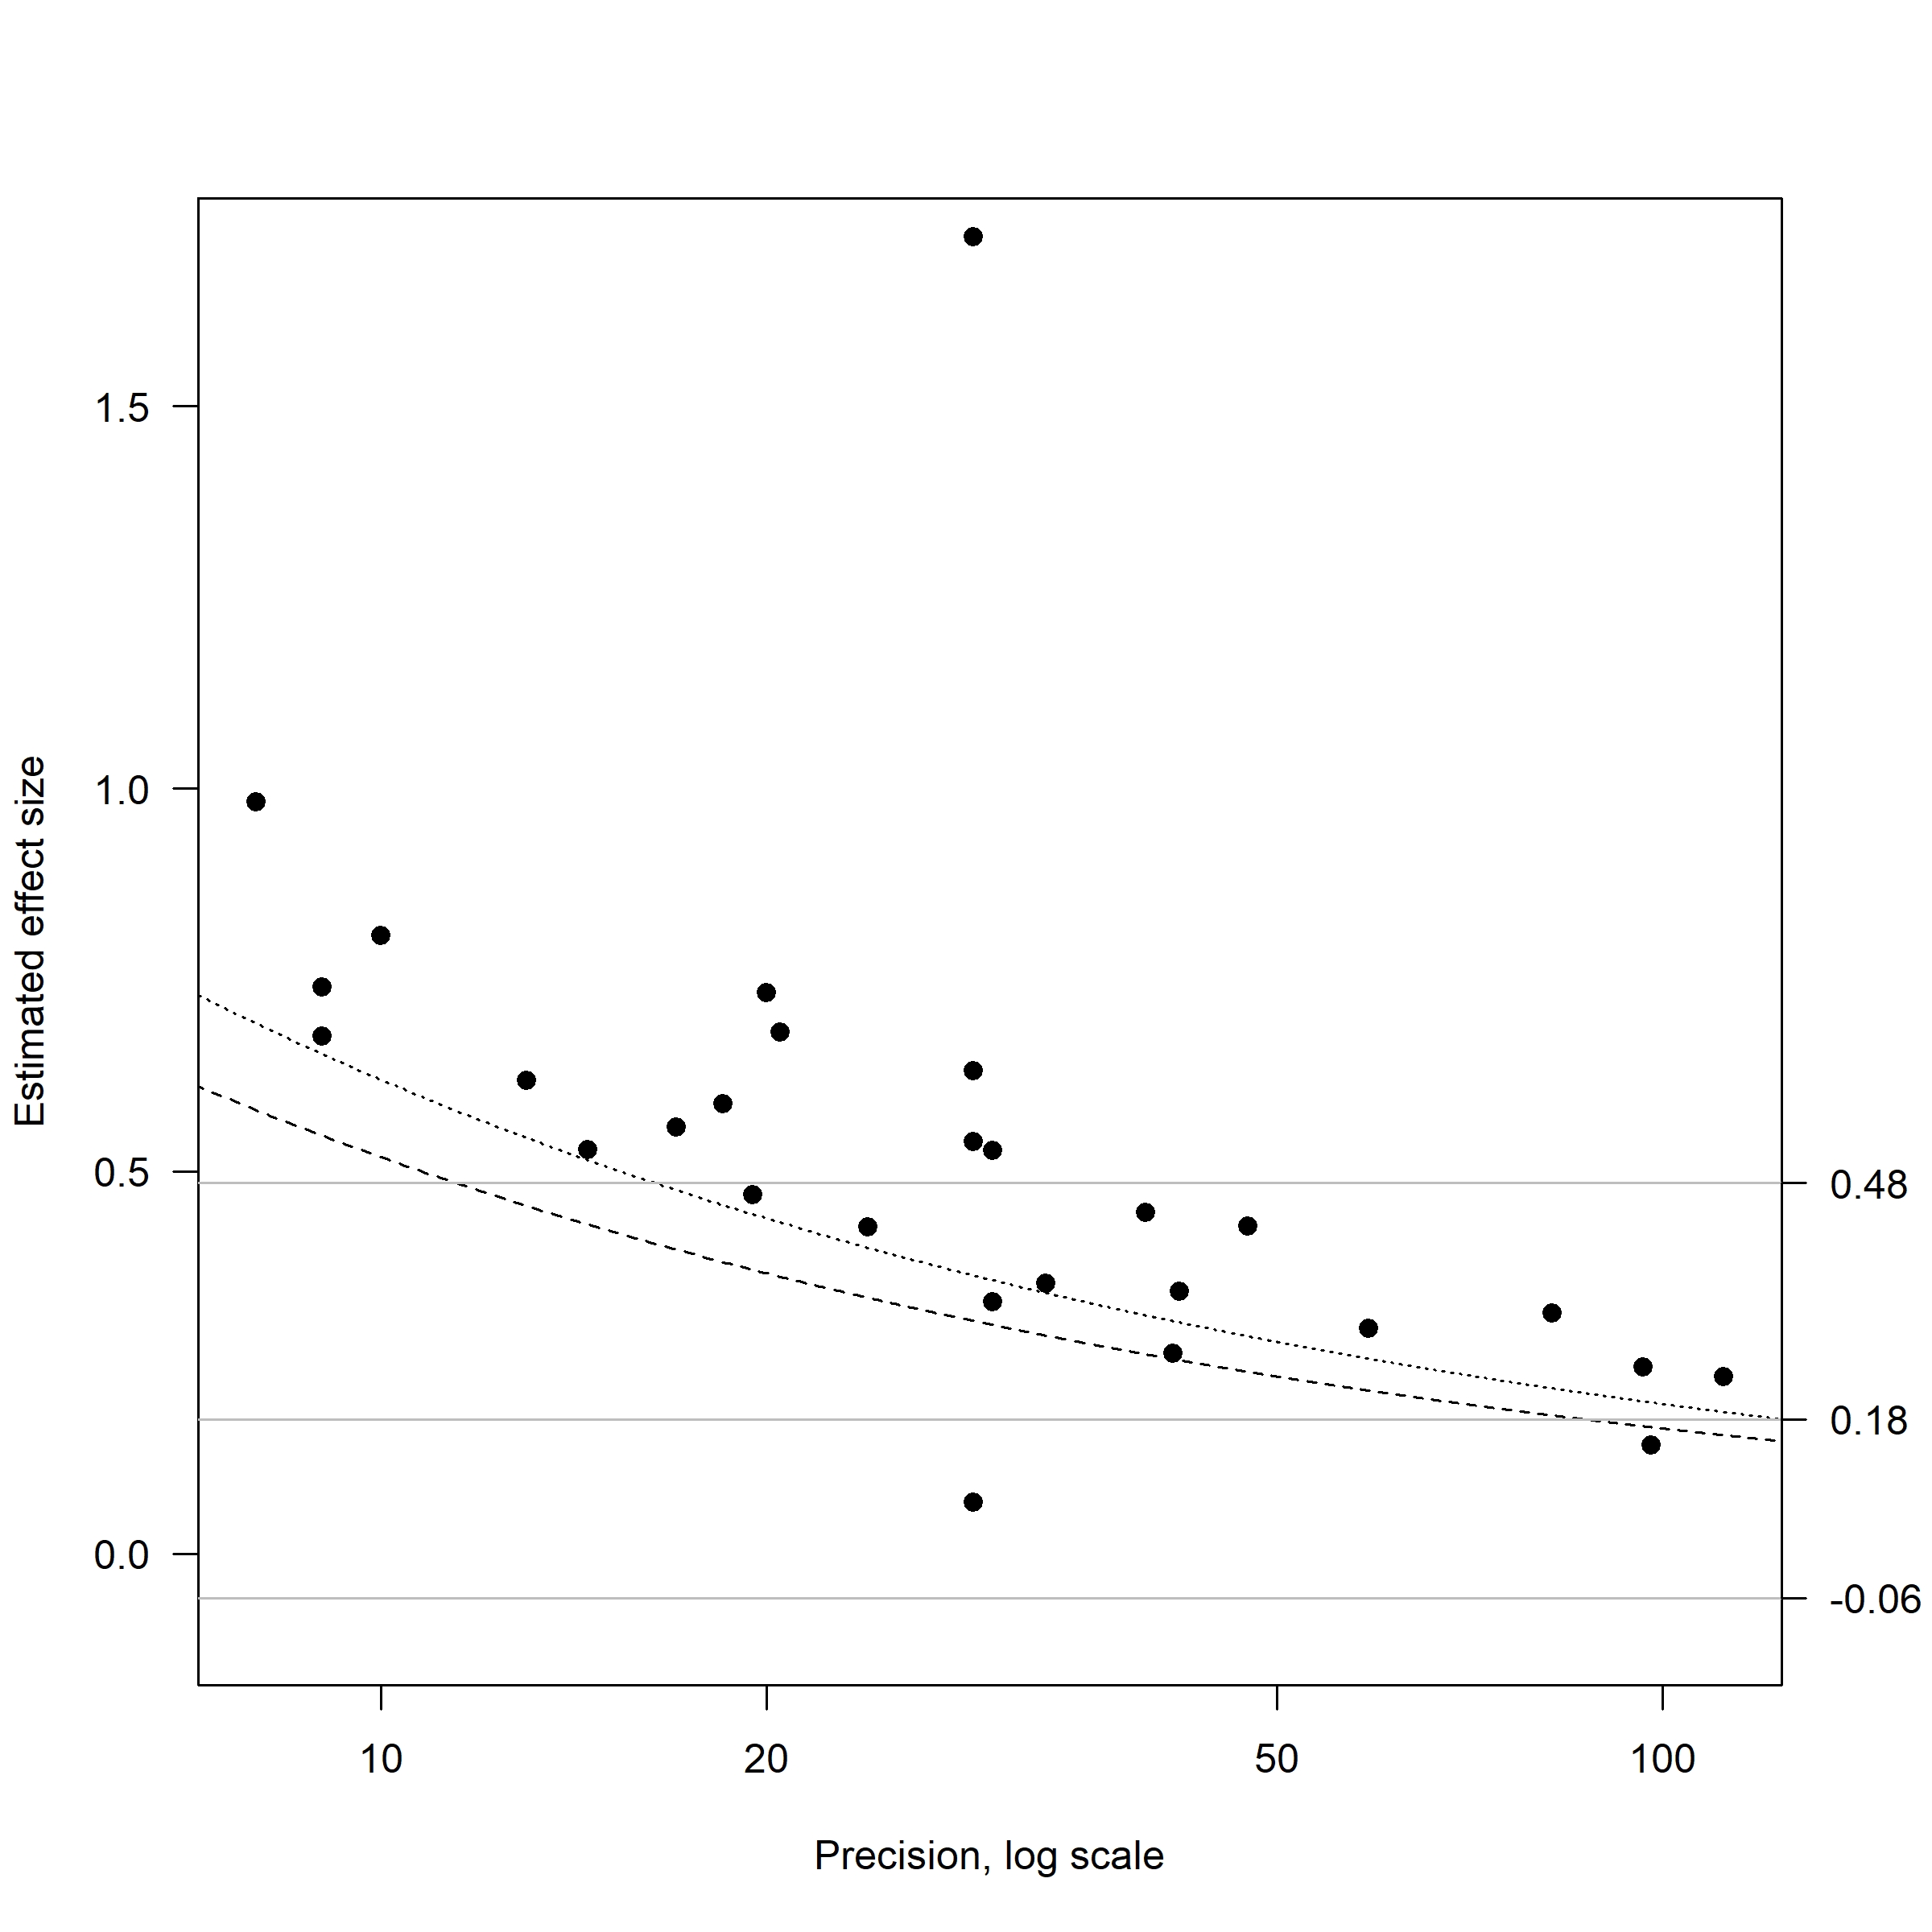
\includegraphics[width=0.49\textwidth]{plots/cuddy2018}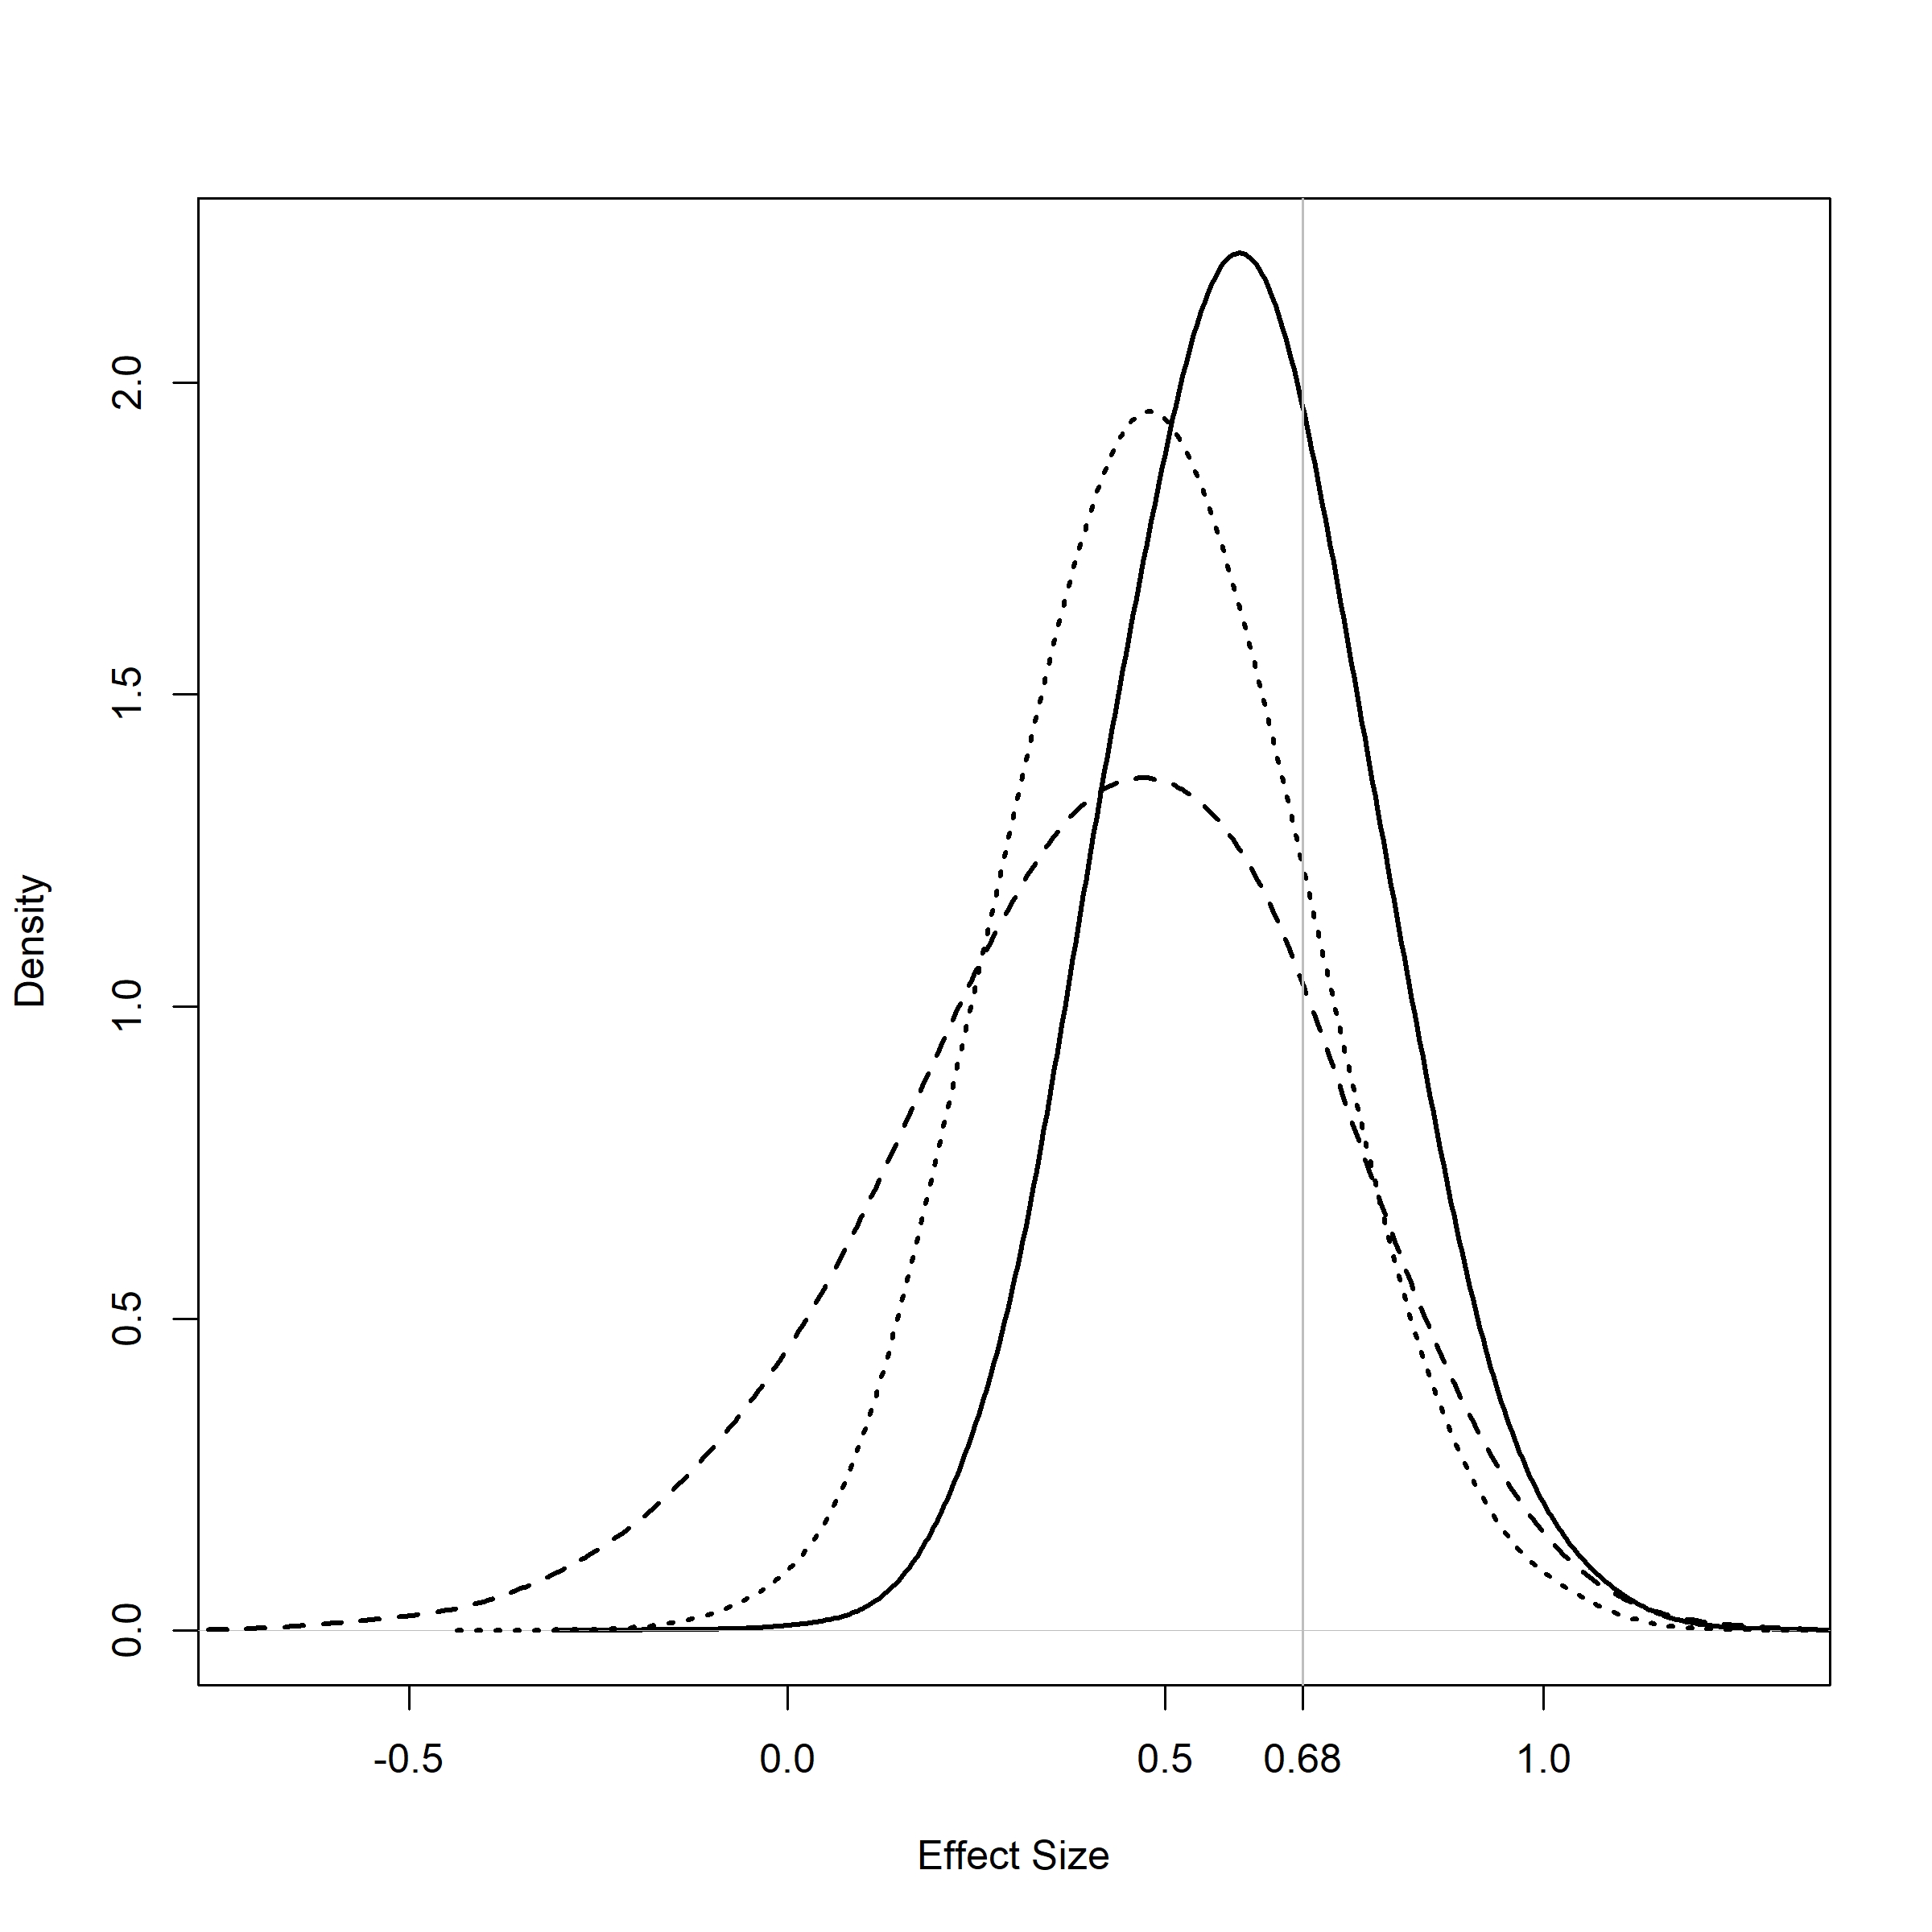
\includegraphics[width=0.49\textwidth]{plots/cuddy2018_posterior}
\par\end{centering}
\caption{\label{fig:cuddy2017} \textbf{(left)} Effect sizes for the power posing example. The dotted black line is $1.96/\textrm{sd}$ and the dashed black line is $1.64/\textrm{sd}$. The ticks on the right hand side are
the meta-analytic means: $0.48$ is from the uncorrected model, $0.17$ is the mean of the selected effect size distribution under the \textit{p}-hacking model, while $-0.06$ is the mean under the publication bias model. \textbf{(right)} Posterior densities for $\theta_{2}$ in the power posing example. The dashed density belongs to the \textit{p}-hacking model, the dotted density to the publication bias model, and the solid density to the uncorrected model. The point $x_{2}=0.62$ is marked for reference.}
\end{figure}

The estimates of the \textit{p}-hacking model, the publication bias model, and the uncorrected meta-analysis models are in Table \ref{tab:cuddy2018}. According to the LOOIC the corrected models account much better for the data than the uncorrected model. Both the \textit{p}-hacking model and the publication bias models estimate
larger $\tau$s and smaller $\theta_{0}$s than the classical model, with the publication bias model estimating the surprising $\theta_{0}\approx0$. But recall the results of the simulation study, where the publication bias model severely underestimates $\theta_0$ when the \textit{p}-hacking model is true.

The publication bias selection affects not only the observed $x_{i}$s, but also the $\theta_{i}$s. As a consequence, the posterior mean of the selected effect size distribution (this equals $0.37$, is not shown in the table, and equals the average of the posterior means for the $\theta_{i}$s) is much closer to the uncorrected model's estimate than the \textit{p}-hacked estimate. This effect can be most easily understood by looking at a specific $\theta$, for example the $\theta_2$ reported in the right plot of Figure \ref{fig:cuddy2017}, where $x_{2}=0.62$. In this case, the publication bias posterior for is close to the uncorrected posterior even though $\theta_0 \approx 0$. On the other hand, the \textit{p}-hacking model pushes $0.62$ down to $0.17$, towards the meta-analytic mean of \DIFdelbegin \DIFdel{$.18$}\DIFdelend \DIFaddbegin \DIFadd{$0.18$}\DIFaddend .

Finally, the surprisingly low value for $\theta_0$ obtained with the publication bias model can be a side effect of the presence of the outlier $x_{12} = 1.72$. Its presence on the right tail of an hypothetical true effect size distribution implies unobserved low and negative effects not reported due to publication bias. When the outlier is removed from the analysis, the estimate of $\theta_{0}$ goes up and agrees with the estimate from the \textit{p}-hacking model, which does not change. Once the outlier is removed, the fit of the publication bias model increases tremenduously, reaching a level close to that of the \textit{p}-hacking model. Moreover, the estimates of $\tau$ are strongly affected by the removal of $x_{12}$. In particular, the estimate of $\tau$ decreases from $0.45$ to $0.09$ in the \textit{p}-hacking model.

%% <<<<< Example table start (\label{tab:cuddy2018)
%% This document is generated by R: DO NOT EDIT BY HAND!
\begin{table}
\caption{\label{tab:cuddy2018} Power posing example: Posterior means for LOOICs and parameters (mean effect $\theta$, standard deviation $\tau$, probabilities of \emph{p}-hacking $\pi$/probabilities of being published $\rho$) of the \emph{p}-hacking, publication bias, and classical meta-analysis (uncorrected) model estimated on the data by \citet{cuddy2018p}. The results in the top table are obtained with all studies, those in the bottom without the outlier $x_{12}$. Posterior standard deviations are reported between brackets.}
\noindent
\begin{center}%
\begin{tabular}{lrrrrrrrrr}
\multicolumn{10}{c}{\bf All studies}\\
  & LOOIC & \multicolumn{1}{c}{$\theta_{0}$} & \multicolumn{1}{c}{$\tau$} & \multicolumn{1}{c}{$\pi_{1}/\rho_{1}$} & \multicolumn{1}{c}{$\pi_{2}/\rho_{2}$} \\ 
  \hline
uncorrected & 16 (18) & 0.48 (0.07) & 0.27 (0.06) &   &   \\ 
  \emph{p}-hacking & -18 (14) & 0.18 (0.12) & 0.45 (0.10) & 0.62 (0.15) & 0.23 (0.14) \\ 
  publication bias & -5.1 (22) & -0.06 (0.23) & 0.37 (0.09) & 0.39 (0.22) & 0.03 (0.03) \\ 
   \hline
\tabularnewline
\multicolumn{10}{c}{\bf Without outlier}\\
  & LOOIC & \multicolumn{1}{c}{$\theta_{0}$} & \multicolumn{1}{c}{$\tau$} & \multicolumn{1}{c}{$\pi_{1}/\rho_{1}$} & \multicolumn{1}{c}{$\pi_{2}/\rho_{2}$} \\ 
  \hline
uncorrected & -7.1 (5.7) & 0.39 (0.04) & 0.09 (0.05) &   &   \\ 
  \emph{p}-hacking & -38 (10) & 0.18 (0.07) & 0.09 (0.07) & 0.62 (0.15) & 0.24 (0.15) \\ 
  publication bias & -35 (11) & 0.16 (0.09) & 0.08 (0.06) & 0.26 (0.17) & 0.03 (0.03) \\ 
   \hline
\end{tabular}
\end{center}
\end{table}

%% example table end >>>>>

In conclusion, the \textit{p}-hacking and publication bias models suggest there is selection bias in these studies. Both models have much better fit than the uncorrected one and it is reasonable to accept their parameter estimates as more realistic. \DIFdelbegin \DIFdel{Nontheless}\DIFdelend \DIFaddbegin \DIFadd{Nonetheless}\DIFaddend , both models agree on a value of $\theta_{0}$ that is likely to be different from $0$. The results of Table \ref{tab:cuddy2018} supports \citet{cuddy2018p}'s conclusion that there is evidence for some positive effect of power posing. The \textit{p}-hacking model does not suffer the presence of an outlier, and, in contrast to the publication bias model, provides similar results with and without $x_{12}$ in the data.

\subsection{Violent video games\label{subsec:Anderson}}

\citet{anderson2010violent} conducted a large meta-analysis on the effects of violent video games on seven negative outcomes such as aggressive behavior and aggressive cognition. As part of their analysis, they classified some experiments as best practice experiments \citep[for more details, see Table 2 of][]{anderson2010violent}. Suspecting publication bias, \citet{hilgard2017overstated} reanalysed the data using an array of tools to detect and adjust for publication bias. For the outcome variable aggressive cognition, \citet{hilgard2017overstated} noted that \enquote{Application of best-practices criteria seems to emphasize statistical significance, and a knot of experiments just reach statistical significance}. The data can be found on the web \citep{Hilgard2017} and are visualised to the left in Figure \ref{fig:anderson2010}. In the plot, the best practice experiments are represented by solid circles, all other experiments by hollow squares. An outlier $x=1.33$ has been removed from the data set, and excluded from our analyses. Its removal substantially improves the fit for all the models. 

In this example we fit the three models (\textit{p}-hacking, publication bias and uncorrected models) to three data subsets (all experiments, only best practice experiments, without best practice experiments). The outcome variable is aggressive behavior. Our the aim is to answer the following: \DIFdelbegin %DIFDELCMD < \begin{enumerate}
%DIFDELCMD < \item %%%
\DIFdelend \DIFaddbegin \DIFadd{(1) }\DIFaddend What are the parameter estimates, in each subset, for each model? \DIFdelbegin %DIFDELCMD < \item %%%
\DIFdelend \DIFaddbegin \DIFadd{(2) }\DIFaddend Which model has the best fit? \DIFdelbegin %DIFDELCMD < \item %%%
\DIFdelend \DIFaddbegin \DIFadd{(3) }\DIFaddend Do we have a reason to believe the best practice experiments are drawn from a different underlying distribution than the other experiments, as \citet{hilgard2017overstated} and the top left plot of Figure \ref{fig:anderson2010} suggest? \DIFdelbegin %DIFDELCMD < \item %%%
\DIFdelend \DIFaddbegin \DIFadd{(4) }\DIFaddend Is there a large difference between the posterior for $\theta_{0}$ and the mean posterior for the $\theta_{i}$s, as we saw in the previous example?
\DIFdelbegin %DIFDELCMD < \end{enumerate}
%DIFDELCMD < %%%
\DIFdelend 

%% <<<<< Example table start (\label{tab:anderson2010)
%% This document is generated by R: DO NOT EDIT BY HAND!
\begin{table}
\noindent
\caption{\label{tab:Anderson2010}Violent video games example: Posterior means for LOOICs and parameters (mean effect $\theta$, standard deviation $\tau$, probabilities of \emph{p}-hacking $\pi$/probabilities of being published $\rho$) of the \emph{p}-hacking, publication bias, and classical meta-analysis (uncorrected) model estimated on the aggressive behavior data from \citet{anderson2010violent}. Posterior standard deviations are reported between brackets.}
\begin{center}%
\begin{tabular}{lcccccccccc}
\multicolumn{11}{c}{\bf All Experiments} \tabularnewline
  & LOOIC & \multicolumn{1}{c}{$\theta_{0}$} & \multicolumn{1}{c}{$\tau$} & \multicolumn{1}{c}{$\pi_{1}/\rho_{1}$} & \multicolumn{1}{c}{$\pi_{2}/\rho_{2}$} \\ 
  \hline
uncorrected & -38 (11) & 0.18 (0.02) & 0.04 (0.03) &   &   \\ 
  \emph{p}-hacking & -48 (13) & 0.09 (0.04) & 0.05 (0.04) & 0.25 (0.11) & 0.23 (0.11) \\ 
  publication bias & -54 (13) & 0.08 (0.03) & 0.03 (0.02) & 0.44 (0.18) & 0.13 (0.07) \\ 
   \hline
\tabularnewline
\multicolumn{11}{c}{\bf Only Best Practice Experiments} \tabularnewline
  & LOOIC & \multicolumn{1}{c}{$\theta_{0}$} & \multicolumn{1}{c}{$\tau$} & \multicolumn{1}{c}{$\pi_{1}/\rho_{1}$} & \multicolumn{1}{c}{$\pi_{2}/\rho_{2}$} \\ 
  \hline
uncorrected & -42 (6.2) & 0.22 (0.02) & 0.03 (0.02) &   &   \\ 
  \emph{p}-hacking & -59 (12) & 0.10 (0.05) & 0.06 (0.04) & 0.37 (0.17) & 0.41 (0.17) \\ 
  publication bias & -61 (11) & 0.11 (0.04) & 0.03 (0.02) & 0.46 (0.21) & 0.06 (0.05) \\ 
   \hline
\tabularnewline
\multicolumn{11}{c}{\bf Without Best Practice Experiments} \tabularnewline
  & LOOIC & \multicolumn{1}{c}{$\theta_{0}$} & \multicolumn{1}{c}{$\tau$} & \multicolumn{1}{c}{$\pi_{1}/\rho_{1}$} & \multicolumn{1}{c}{$\pi_{2}/\rho_{2}$} \\ 
  \hline
uncorrected & -7.4 (5.7) & 0.06 (0.04) & 0.08 (0.05) &   &   \\ 
  \emph{p}-hacking & -6.2 (5.1) & 0.01 (0.05) & 0.07 (0.05) & 0.10 (0.07) & 0.11 (0.08) \\ 
  publication bias & -7.7 (5) & 0.02 (0.04) & 0.06 (0.04) & 0.61 (0.23) & 0.35 (0.19) \\ 
   \hline
\end{tabular}
\end{center}
\end{table}

%% example table end >>>>>

The first three questions can be answered by looking at Table \ref{tab:Anderson2010}. The estimates of $\theta_{0}$ are approximately the same for the publication bias and \textit{p}-hacking models, and roughly half of the uncorrected estimate in all cases. In particular, when all experiments or only the best experiments are considered, there is a noticeable difference. In these two cases, the LOOICs suggest that some \textit{p}-hacking or publication bias is present, as they are smaller than the LOOIC for the uncorrected models. Although the publication bias model seems to work slightly better than the \textit{p}-hacking model, we can state that the two models agree and we have little reason to prefer one to the other. Basically, we can interpret this as converging evidence that the parameter estimates obtained with these two models for $\theta_{0}$ and $\tau$ are in the ballpark of their true values.

Interestingly, when we exclude the experiments not considered best practice by \citet{anderson2010violent}, the differences between the estimates provided by the corrected and uncorrected models reduce and the LOOICs are almost the same. The question is if the differences between best practice and non-best practice studies reflect a different underlying distribution or not. To answer this question, let us take a look at the posterior densities for $\theta_{0}$ when all experiments are included, as reported in the top right plot of Figure \ref{fig:anderson2010}. In this case, the posterior distributions computed with the \textit{p}-hacking and publication bias models are similar (dashed and dotted lines, respectively), which strengthens the agreement seen in Table \ref{tab:Anderson2010}. There is no large difference between the posterior for $\theta_{0}$ and the mean posterior for the $\theta_{i}$s as in the previous example. The answer to question (4) is therefore no.

Back to question (3)\DIFdelbegin \DIFdel{. We }\DIFdelend \DIFaddbegin \DIFadd{, we }\DIFaddend have good reasons to believe the best practice experiments have been drawn from a different underlying distribution than the other experiments if there is negligible overlap between the posteriors for the parameters $\theta_{0}$. The uncorrected model supports this hypothesis (bottom right plot of Figure \ref{fig:anderson2010}), but the \textit{p}-hacking and publication bias models to do not. See the bottom left plot of Figure \ref{fig:anderson2010} for the posteriors for $\theta_0$ in the publication bias model (those obtained with the \textit{p}-hacking model are indistinguishable). In this case, the overlap between the posteriors for the different subsets is not negligible, and there is no evidence against hypotheses of equal $\theta_0$s in both groups. The same conclusion can be reached from Table \ref{tab:Anderson2010} by looking at the posterior standard deviations and posterior means.

\begin{figure}
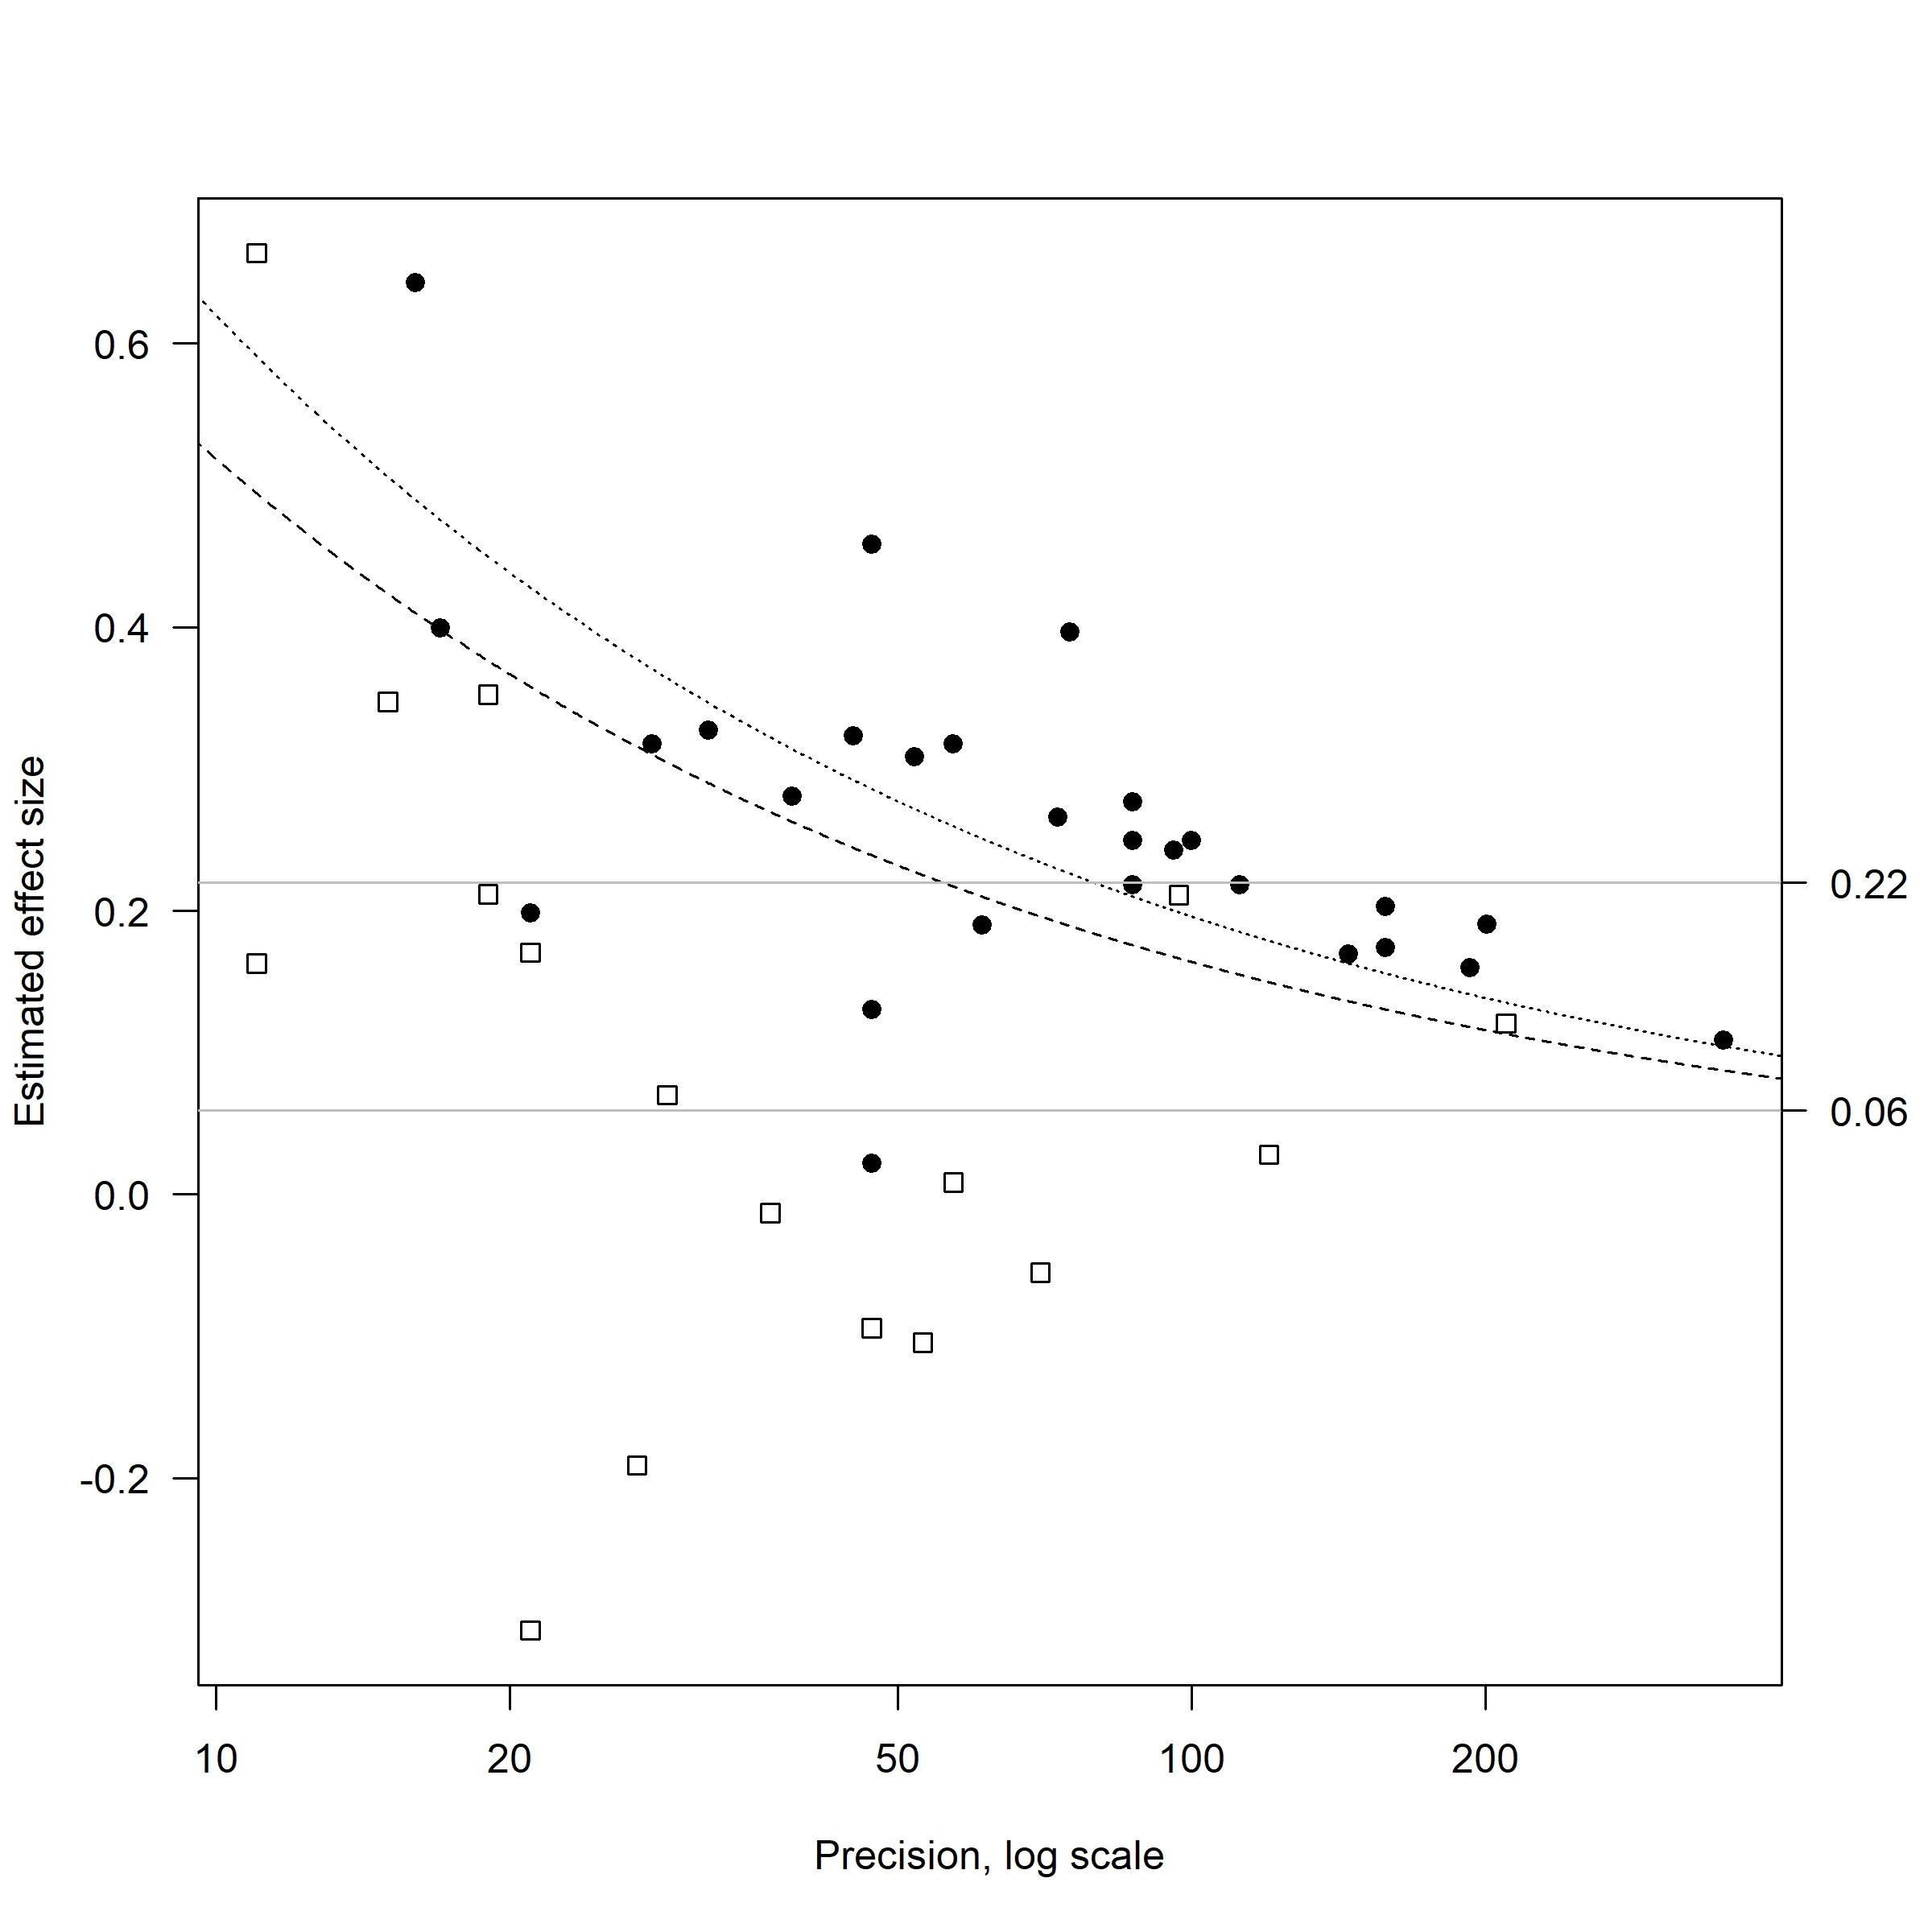
\includegraphics[width=0.49\textwidth]{plots/anderson2010}
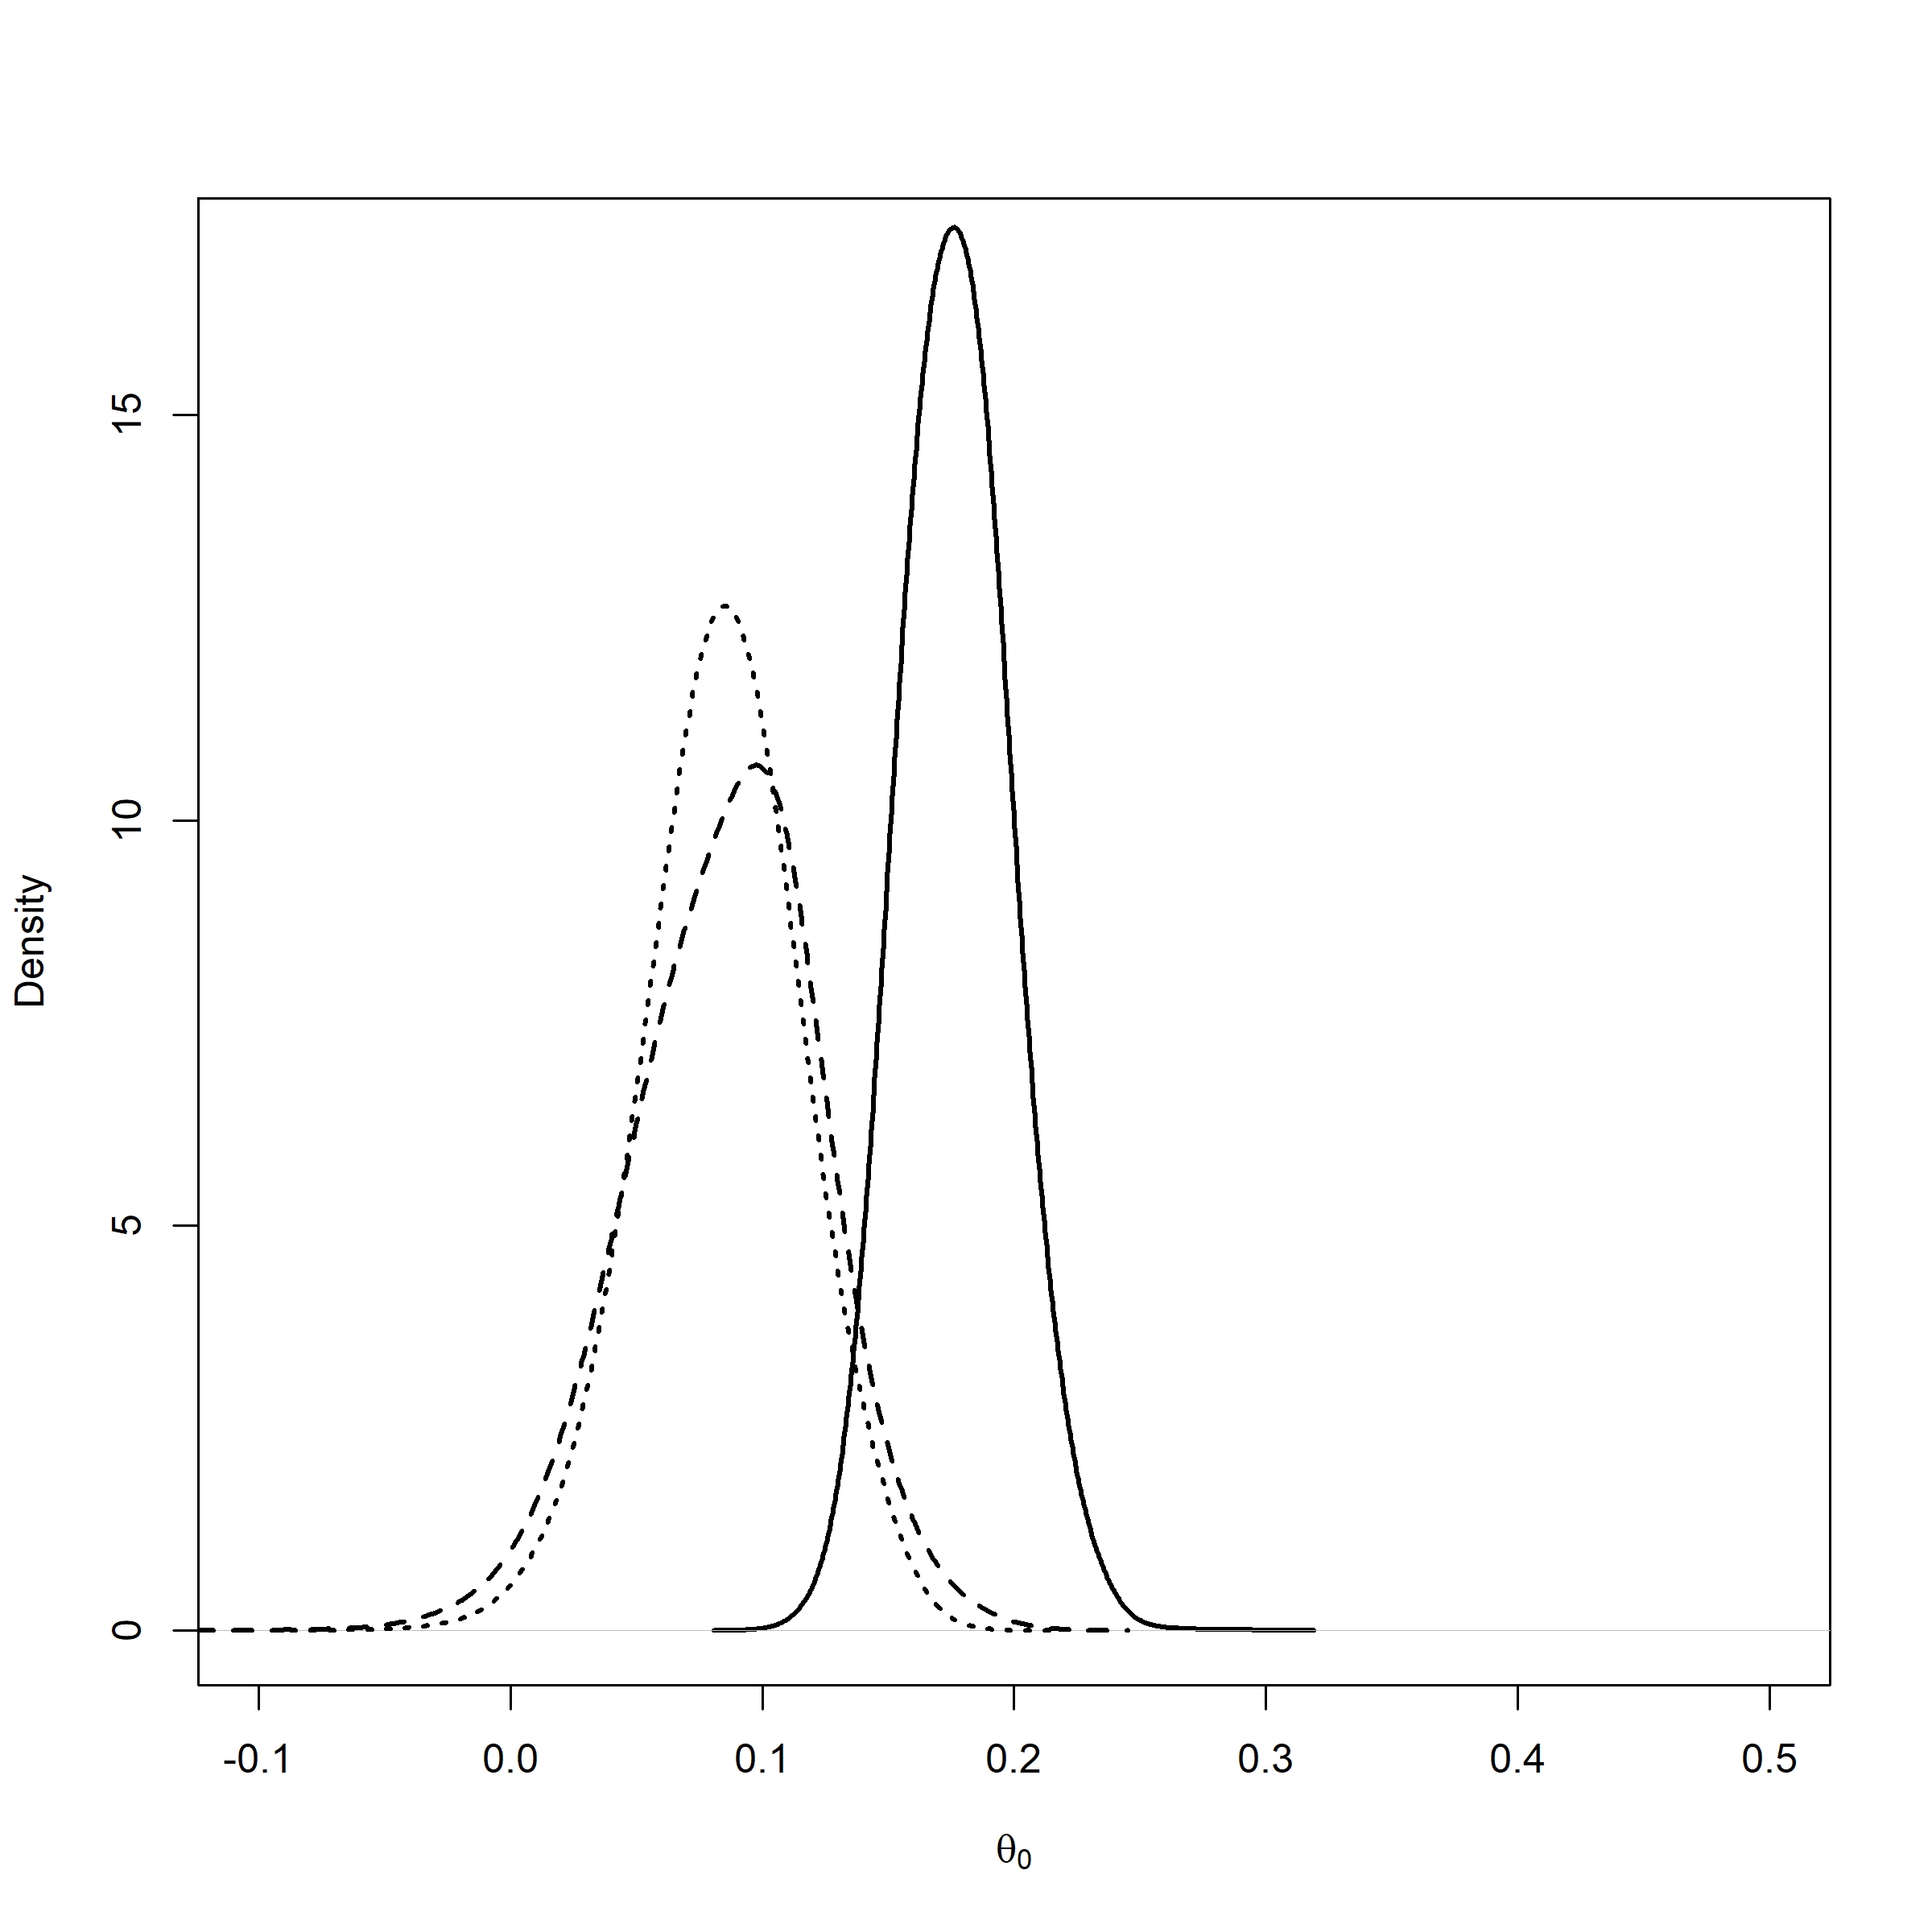
\includegraphics[width=0.49\textwidth]{plots/anderson_posterior}
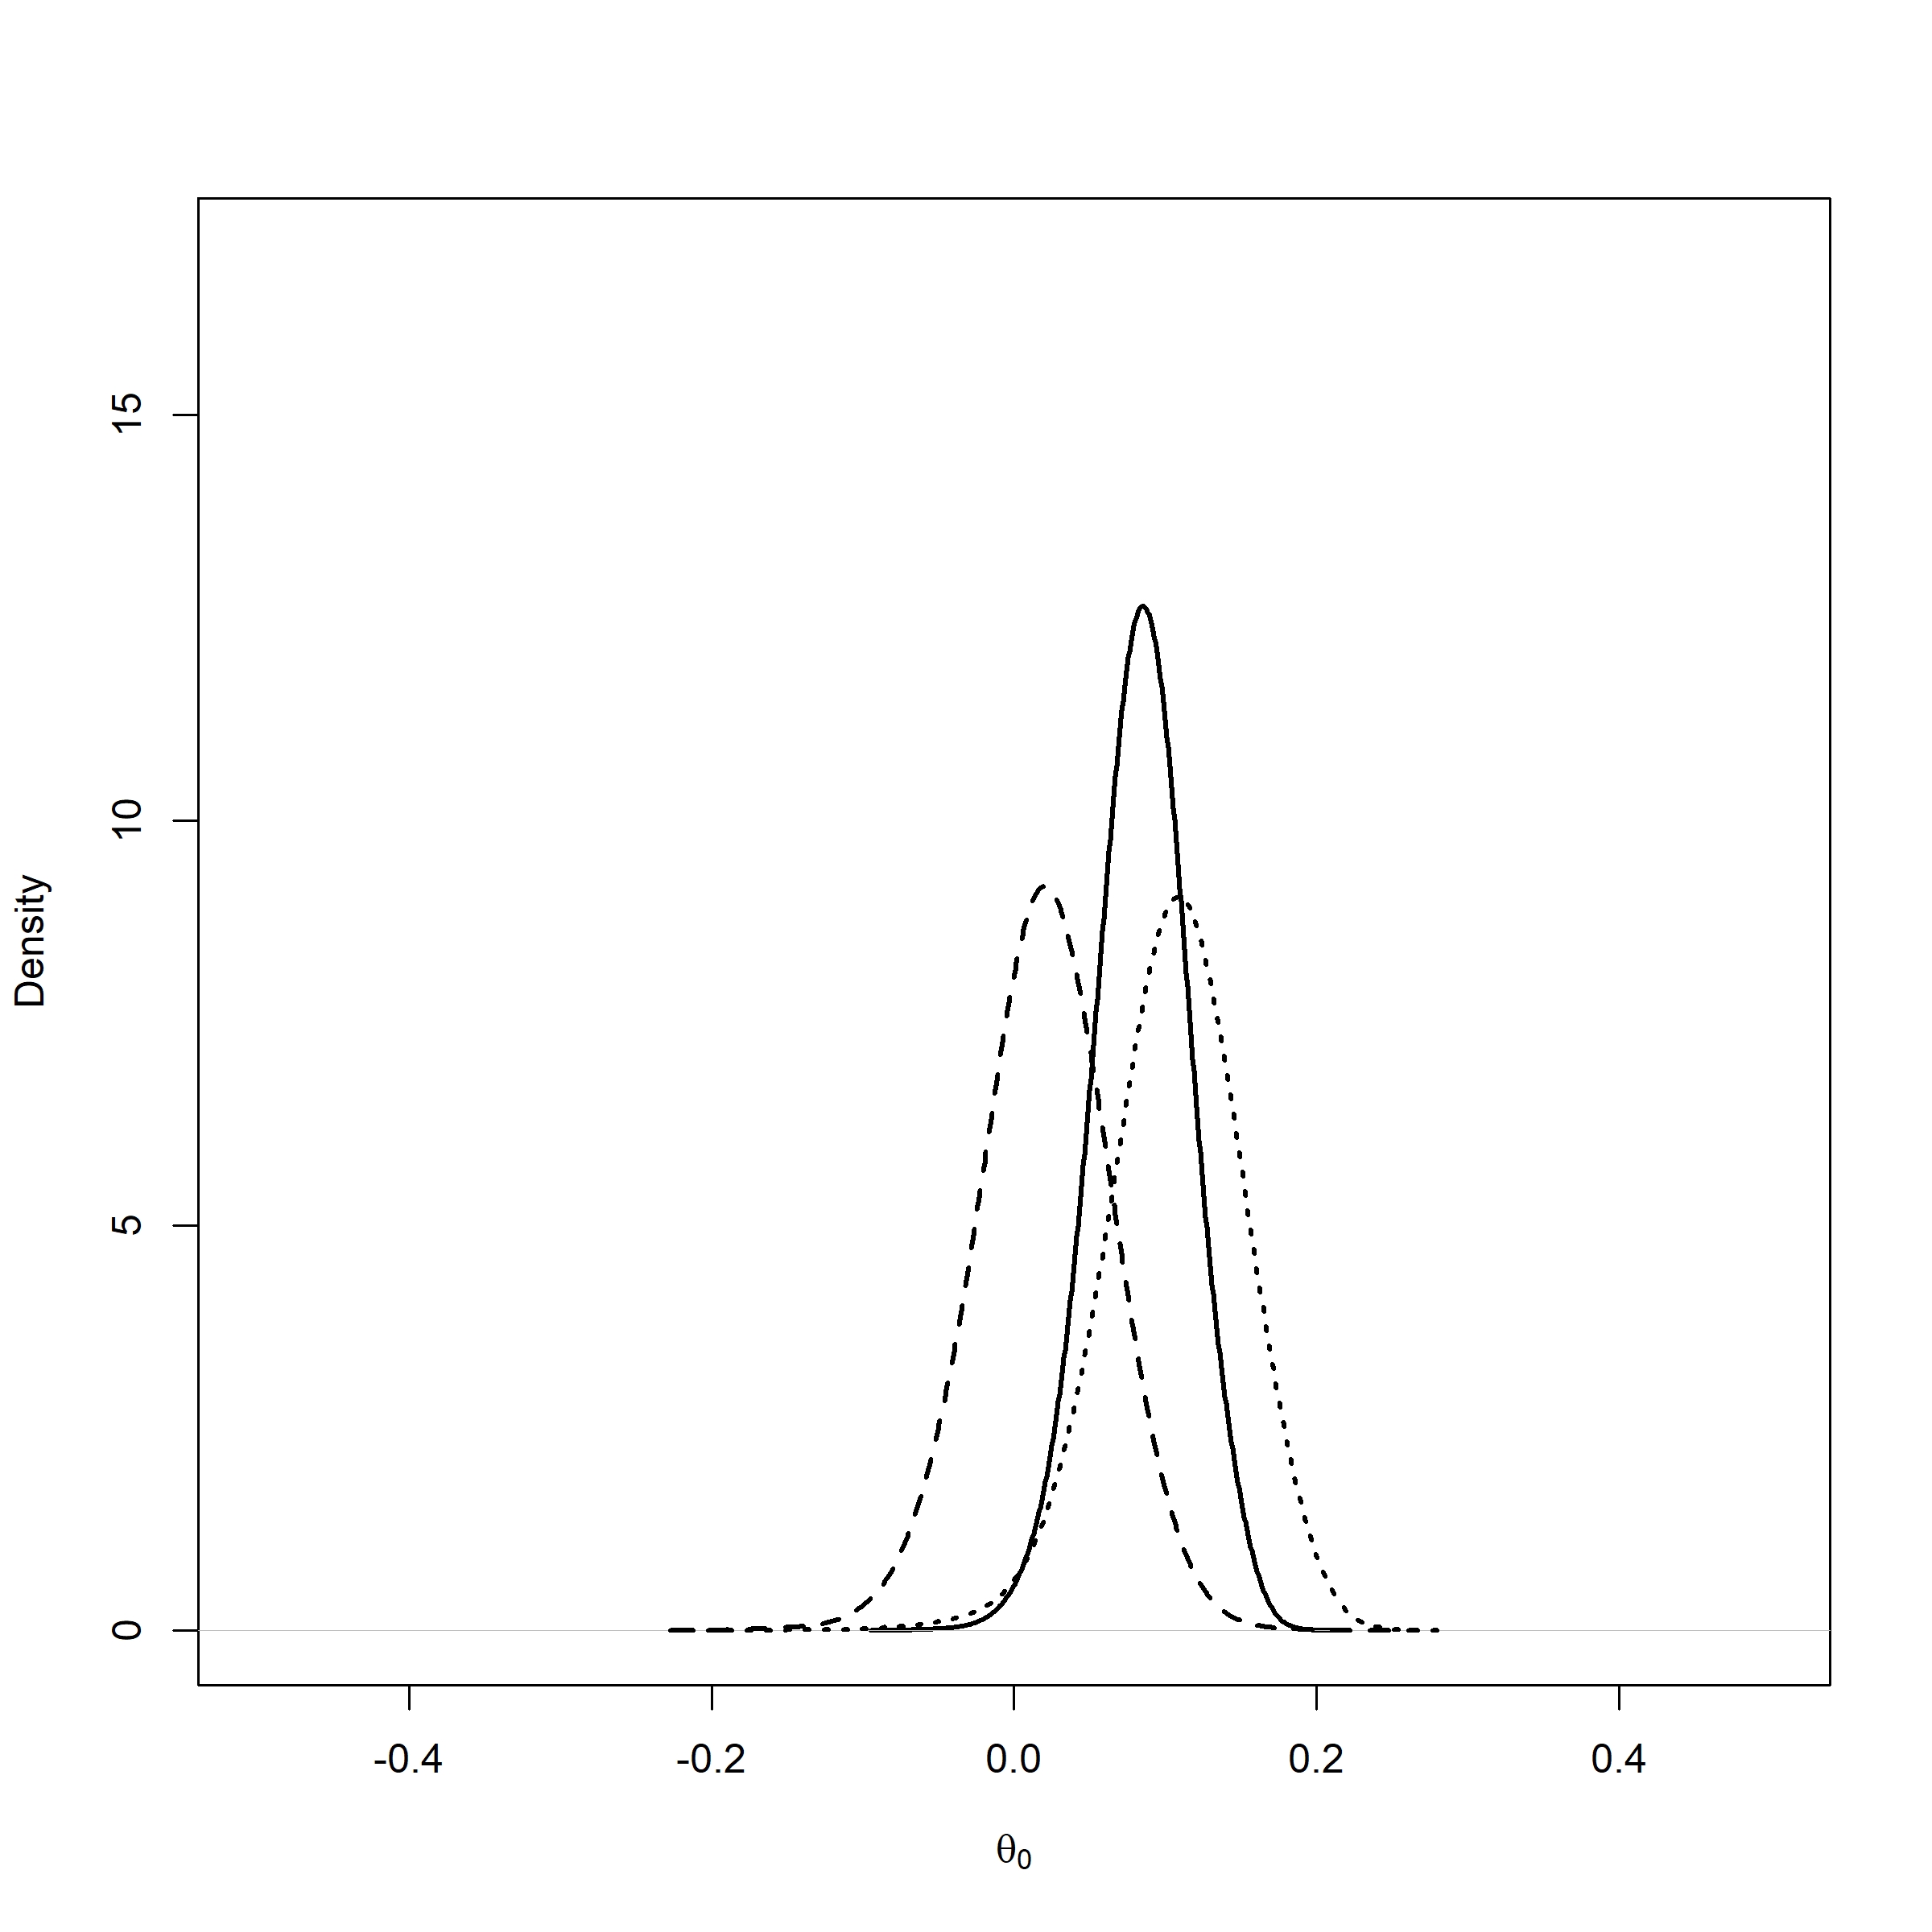
\includegraphics[width=0.49\textwidth]{plots/anderson_posterior_1}
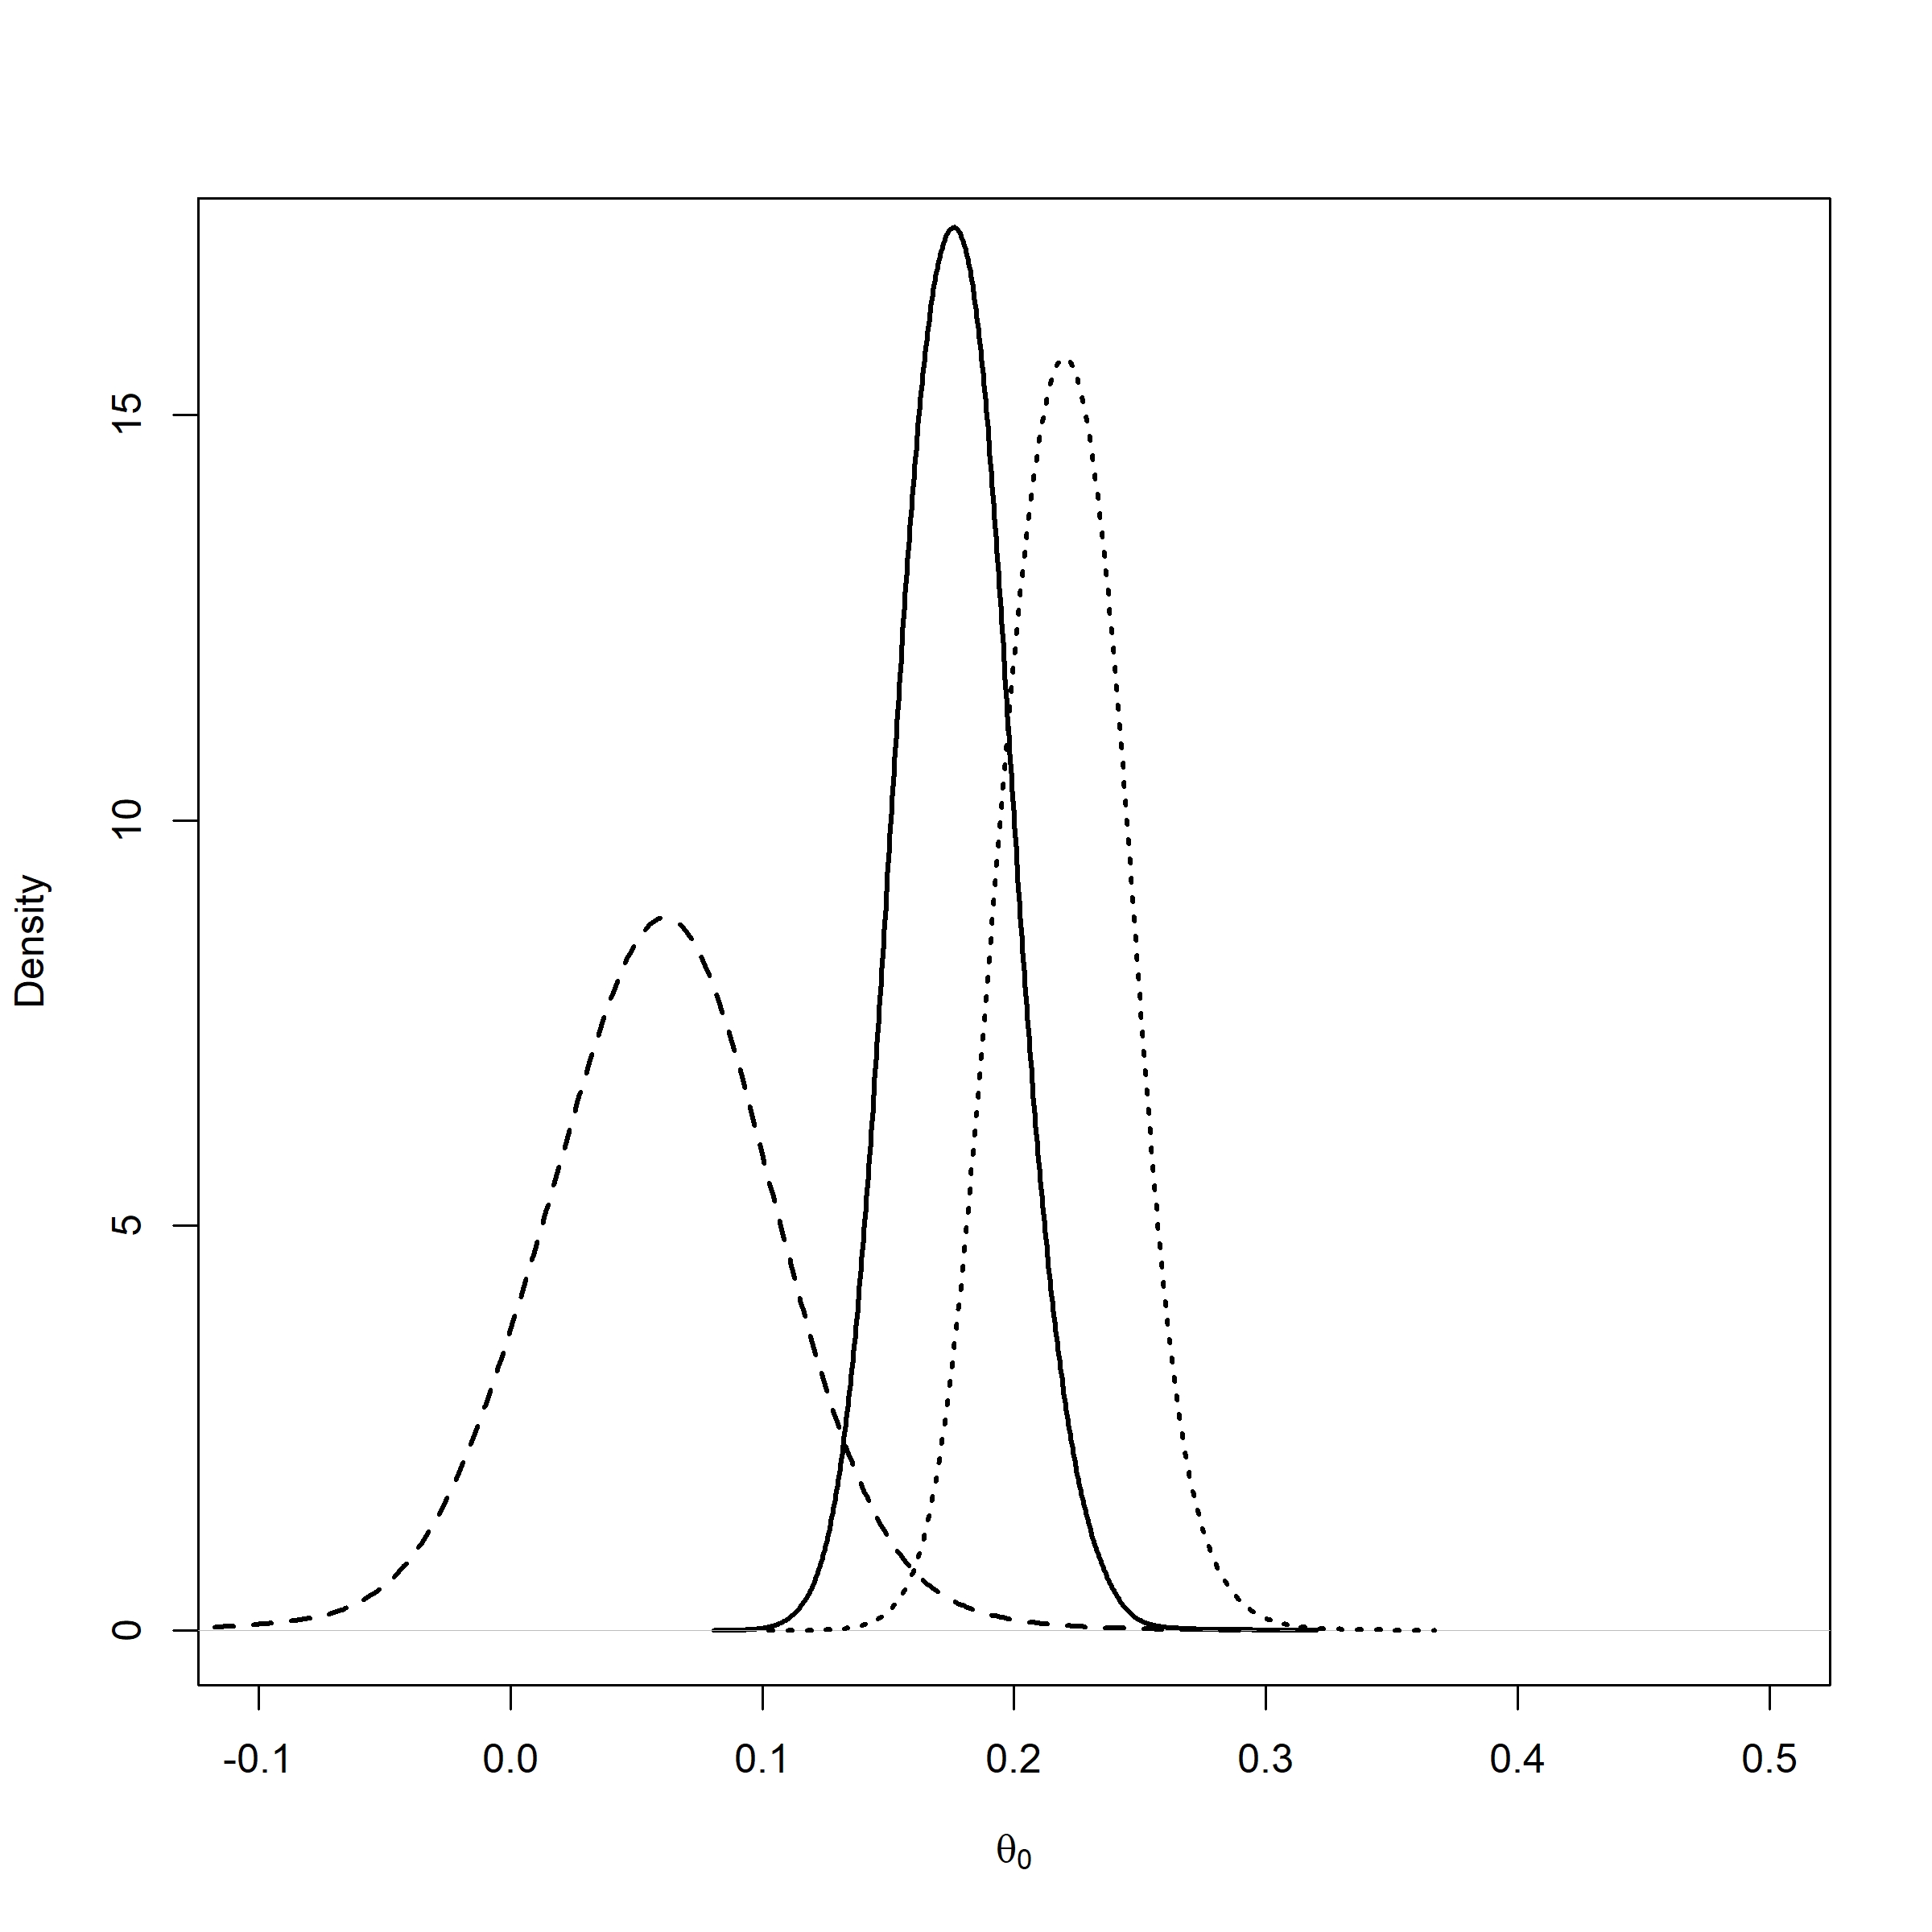
\includegraphics[width=0.49\textwidth]{plots/anderson_posterior_2}
\caption{\label{fig:anderson2010}Violent video games example with outcome variable aggressive behavior. \textbf{(top-left)} Effect sizes. The dotted black line is $1.96/\textrm{sd}$ and the dashed black line is $1.64/\textrm{sd}$. The ticks on the right hand side are the uncorrected meta-analytical means for each group: $0.29$ for the best practices group, $0.08$ for the rest. The outlier $x=1.33$ has been removed from the plot.
\textbf{(top-right)} Posterior densities for $\theta_{0}$ with all experiments included. The dashed density belongs to the \textit{p}-hacking model, the dotted to the publication bias model, and the solid to the uncorrected model. \textbf{(bottom-left)} Posterior densities for $\theta_{0}$ from the publication bias model. The solid curve is the model with all experiments, the dotted curve the model with the best practice experiments, and the dashed line the model without the best experiments. The posteriors for the \textit{p}-hacking model are similar to this one. \textbf{(bottom-right)} Posterior densities for $\theta_{0}$ (solid line: all experiments; dotted line: best practice experiments only; and dashed line without the best experiments) from the uncorrected meta-analysis model.}
\end{figure}

\section{Concluding remarks}\label{sect:conclusions}

In this paper we studied two models to handle the effect of \textit{p}-hacking and publication bias. Although the \textit{p}-hacking model worked really well in the simulation study, we have to admit that the \textit{p}-hacking scenario described in \DIFdelbegin \DIFdel{section }\DIFdelend \DIFaddbegin \DIFadd{Section }\DIFaddend \ref{subsect:p-hacking} is less plausible than the publication bias scenario of \DIFdelbegin \DIFdel{section }\DIFdelend \DIFaddbegin \DIFadd{Section }\DIFaddend \ref{subsect:publicationBias}. First, the assumption of Bob's \textit{p}-hacking omnipotence is strong. For while some researchers are able \textit{p}-hackers, most give up at some point. Does truncation actually model \textit{p}-hacking in the wild? Analysing \textit{p}-hacking is hard without serious simplifying assumptions. The model we proposed is interpretable and implementable, and it appears to work well in practice, as one can see in the examples of \DIFdelbegin \DIFdel{section }\DIFdelend \DIFaddbegin \DIFadd{Section }\DIFaddend \ref{sect:examples}. That said, there is space for further development of models for \textit{p}-hacking.

Regarding possible further development, we are often interested in understanding and modelling the sources of heterogeneity in a meta-analysis \citep{thompson1994systematic}. A way to do this is to let $\theta_{i}$ linearly depend on covariates, in the meta-analysis context known as moderators. If we extend the one-sided discrete models publication bias and \textit{p}-hacking models to include covariates, we will be able to estimate their effect while keeping the \textit{p}-hacking probability or the selection probability fixed. Another option is to allow the \textit{p}-hacking probability or the selection probability to depend on covariates themselves. For instance, the difficulty of \textit{p}-hacking is likely to increase with $n$, the sample size of the study. Similarly, the selection probability is also likely to be influenced by $n$; for example when $n$ is large, null-effects are more publishable.

\DIFdelbegin \DIFdel{The notation introduced in section \ref{sec:Selection Sets} can be used to visualize modifications of the two concrete models used in this paper, as in Figure \ref{fig:Plate notation, publication bias and p-hacking}. In }\DIFdelend \DIFaddbegin \DIFadd{Further modification to }\DIFaddend the \DIFaddbegin \DIFadd{models can be obtained by modifying their selection sets. For example, in the }\DIFaddend publication bias model, the nuisance parameter \DIFdelbegin \DIFdel{$\eta$ }\DIFdelend \DIFaddbegin \DIFadd{$\eta_i$ }\DIFaddend (which can include, e.g., the standard deviation \DIFdelbegin \DIFdel{$\sigma$}\DIFdelend \DIFaddbegin \DIFadd{$\sigma_i$}\DIFaddend ) could be \DIFdelbegin \DIFdel{put inside the selection plate. In this case, new $\eta$s are drawn until a studyis accepted}\DIFdelend \DIFaddbegin \DIFadd{incorporated. Although the common practice in meta-analysis studies is to treat the standard deviations as nuisance parameter \mbox{%DIFAUXCMD
\citep[see, e.g.,][]{vanHouwelingen2002}}\hspace{0pt}%DIFAUXCMD
, the actual tests usually contain an estimate of the standard error. If the $\eta_i$s are in the selection set, they can influence the study's acceptance}\DIFaddend . A possible modification of the \textit{p}-hacking model consists in putting \DIFdelbegin \DIFdel{$\theta$ }\DIFdelend \DIFaddbegin \DIFadd{$\theta_i$ }\DIFaddend inside the selection set, which makes the researcher draw new \DIFdelbegin \DIFdel{$\theta$}\DIFdelend \DIFaddbegin \DIFadd{$\theta_i$}\DIFaddend s every time he attempts a \textit{p}-hack. This could be used to model scenarios where the hypothesis is not known in advance by the researchers.

We saw in the simulations and in Example \ref{subsec:cuddy2018} that the publication bias and the \textit{p}-hacking models can give remarkably different results even with similar priors and the same $\alpha$ vector. A way to react to this situation is to choose the best-fitting model in terms of, for example, LOOIC. Nevertheless, this may result dangerous, and one should be caution, to not risk to over-interpret the results. More safely, one can present the results of both models and try to understand the differences between them, as we did in the examples of \DIFdelbegin \DIFdel{section }\DIFdelend \DIFaddbegin \DIFadd{Section }\DIFaddend \ref{sect:examples}. In the publication bias model, it is especially important to be aware of the interpretation of $\theta_{0}$ as the mean of the underlying effect size distribution, not the effect size distribution of the observed studies. Therefore, the best response to the question \enquote{Should one use the \textit{p}-hacking and publication bias model?} is probably \enquote{Use both!}

Finally, it would be interesting to model publication bias and \textit{p}-hacking at the same time:
\begin{quote}
Bob \textit{p}-hacks his research to a \textit{p}-value drawn from $\omega$ and sends it to Alice's journal. Alice accepts the paper with probability \DIFdelbegin \DIFdel{$w(u)$}\DIFdelend \DIFaddbegin \DIFadd{$w(u_i)$}\DIFaddend . Every rejected study is lost.
\end{quote}
In this scenario the original density $f^{\star}(x_{i}\mid\theta_{i},\eta_{i})$ is transformed twice: First by \textit{p}-hacking, then by publication bias. The resulting model is
$$
f(x_{i}\mid\theta_{i},\eta_{i})\propto w(u\DIFaddbegin \DIFadd{_i}\DIFaddend )\int_{[0,1]}f_{[0,\alpha]}^{\star}(x_{i}\mid\theta_{i},\eta_{i})d\omega(\alpha).
$$
This is a reasonable model, but its normalizing constant is hard to calculate, even when $\omega$ is discrete and $w$ is a step function. Additional work on this problem is required.

%DIFDELCMD < %%%
\DIFdelend \bibliographystyle{biom}
\DIFdelbegin %DIFDELCMD < \bibliography{main.bib}
%DIFDELCMD < %%%
\DIFdelend \DIFaddbegin \bibliography{edited.bib}
\DIFaddend 

\label{lastpage}
\end{document}
